%%%%%%%%%%%%%%%%%%%%%%%%%%%%%%%%%%%%%%%%%
% Masters/Doctoral Thesis 
% LaTeX Template
% Version 2.4 (22/11/16)
%
% This template has been downloaded from:
% http://www.LaTeXTemplates.com
%
% Version 2.x major modifications by:
% Vel (vel@latextemplates.com)
%
% This template is based on a template by:
% Steve Gunn (http://users.ecs.soton.ac.uk/srg/softwaretools/document/templates/)
% Sunil Patel (http://www.sunilpatel.co.uk/thesis-template/)
%
% Template license:
% CC BY-NC-SA 3.0 (http://creativecommons.org/licenses/by-nc-sa/3.0/)
%
%%%%%%%%%%%%%%%%%%%%%%%%%%%%%%%%%%%%%%%%%

%----------------------------------------------------------------------------------------
%	PACKAGES AND OTHER DOCUMENT CONFIGURATIONS
%----------------------------------------------------------------------------------------

\documentclass[
11pt, % The default document font size, options: 10pt, 11pt, 12pt
%oneside, % Two side (alternating margins) for binding by default, uncomment to switch to one side
english, % ngerman for German
singlespacing, % Single line spacing, alternatives: onehalfspacing or doublespacing
%draft, % Uncomment to enable draft mode (no pictures, no links, overfull hboxes indicated)
%nolistspacing, % If the document is onehalfspacing or doublespacing, uncomment this to set spacing in lists to single
%liststotoc, % Uncomment to add the list of figures/tables/etc to the table of contents
%toctotoc, % Uncomment to add the main table of contents to the table of contents
%parskip, % Uncomment to add space between paragraphs
%nohyperref, % Uncomment to not load the hyperref package
headsepline, % Uncomment to get a line under the header
%chapterinoneline, % Uncomment to place the chapter title next to the number on one line
%consistentlayout, % Uncomment to change the layout of the declaration, abstract and acknowledgements pages to match the default layout
]{MastersDoctoralThesis} % The class file specifying the document structure

\usepackage[utf8]{inputenc} % Required for inputting international characters
\usepackage[T1]{fontenc} % Output font encoding for international characters

\usepackage{palatino} % Use the Palatino font by default

\usepackage[backend=bibtex,natbib=true]{biblatex} % Use the bibtex backend with the authoryear citation style (which resembles APA)
%\bibliographystyle{utphys}%hunsrt}%{hep}%{unsrt}

\addbibresource{biblio.bib} % The filename of the bibliography

\usepackage[autostyle=true]{csquotes} % Required to generate language-dependent quotes in the bibliography
\usepackage{ amssymb }
\usepackage{amsmath}

\hyphenation{strange-ness}
%----------------------------------------------------------------------------------------
%	MARGIN SETTINGS
%----------------------------------------------------------------------------------------
\newcommand{\der}{\rm d}
\newcommand{\pp}{p-p}
\newcommand{\sqrts}{\sqrt{s}}
\newcommand{\sqrtsNN}{\sqrt{s_{\rm \scriptscriptstyle NN}}}
\newcommand{\lsim}{\,{\buildrel < \over {_\sim}}\,}
\newcommand{\gsim}{\,{\buildrel > \over {_\sim}}\,}
\newcommand{\av}[1]{\left\langle #1 \right\rangle}
\newcommand{\eV}{\mathrm{eV}}
\newcommand{\keV}{\mathrm{keV}}
\newcommand{\MeV}{\mathrm{MeV}}
\newcommand{\GeV}{\mathrm{GeV}}
\newcommand{\Gevc}{\mathrm{GeV}/c}
\newcommand{\Gevcc}{\mathrm{GeV}/c^{2}}
\newcommand{\TeV}{\mathrm{TeV}}
\newcommand{\ev}{\mathrm{eV}}
\newcommand{\kev}{\mathrm{keV}}
\newcommand{\mev}{\mathrm{MeV}}
\newcommand{\gev}{\mathrm{GeV}}
\newcommand{\tev}{\mathrm{TeV}}
\newcommand{\fm}{\mathrm{fm}}
\newcommand{\mm}{\mathrm{mm}}
\newcommand{\cm}{\mathrm{cm}}
\newcommand{\m}{\mathrm{m}}
\newcommand{\mum}{\mathrm{\mu m}}
\newcommand{\s}{\mathrm{s}}
%\renewcommand{\d}{\mathrm{d}}
\newcommand{\ns}{\mathrm{ns}}
\newcommand{\mrad}{\mathrm{mrad}}
\newcommand{\mb}{\mathrm{mb}}
\newcommand{\mub}{\mathrm{\mu b}}
\newcommand{\T}{\mathrm{T}}
\newcommand{\PbPb}{\mbox{Pb--Pb}}
\newcommand{\Npart}{N_{\rm part}}
\newcommand{\Ncoll}{N_{\rm coll}}
\newcommand{\Raa}{R_{\rm AA}}
\newcommand{\RAA}{R_{\rm AA}}
\newcommand{\TAA}{T_{\rm AA}}
\newcommand{\RCP}{R_{\rm CP}}
\newcommand{\pt}{p_{\rm T}}
\newcommand{\avpt}{\langle p_{\rm t} \rangle}
\newcommand{\dNdy}{{\rm d}N_{ch}/{\rm d}y}
\newcommand{\momwin}{[$p$, $p$+$\Delta$ $p$]}
\newcommand{\DtoKpi}{{\rm D^0\to K^-\pi^+}}
\newcommand{\DtoKpipi}{{\rm D^+\to K^-\pi^+\pi^+}}
\newcommand{\DstartoDpi}{{\rm D^{*+}\to D^0\pi^+}}
\newcommand{\Dzero}{{\rm D^0}}
\newcommand{\Dstar}{{\rm D^{*+}}}
\newcommand{\Dplus}{{\rm D^+}}
\newcommand{\Ds}{{\rm D_s}}
\newcommand{\Dsplus}{{\rm D_s^+}}
\newcommand{\DstoKKpi}{{\rm D^{+}_\mathrm{s}\to K^+ K^-\pi^+}}
\newcommand{\DplustoKKpi}{{\rm D^{+}\to K^+ K^-\pi^+}}
\newcommand{\nbinv}{{\rm nb^{-1}}}
\newcommand{\decleng}{{\rm L}_{xyz}}
\newcommand{\dEdx}{{\rm d}E/{\rm d}x}
\newcommand{\mufac}{\mu_{\rm F}}
\newcommand{\muren}{\mu_{\rm R}}
\newcommand{\vtwo}{\rm v_2}
\newcommand{\sNN}{\sqrt{s_{\rm NN}}}
\newcommand{\Nch}{N_{\rm ch}}
\geometry{
	paper=a4paper, % Change to letterpaper for US letter
	inner=2.5cm, % Inner margin
	outer=3.8cm, % Outer margin
	bindingoffset=.5cm, % Binding offset
	top=1.5cm, % Top margin
	bottom=1.5cm, % Bottom margin
	%showframe, % Uncomment to show how the type block is set on the page
}

%----------------------------------------------------------------------------------------
%	THESIS INFORMATION
%----------------------------------------------------------------------------------------

\thesistitle{Prompt $\Dsplus$ meson production in pp, p-Pb and Pb-Pb collisions at LHC with ALICE} % Your thesis title, this is used in the title and abstract, print it elsewhere with \ttitle
\supervisor{Prof. Stefania Beole'\\ Dr. Francesco Prino} % Your supervisor's name, this is used in the title page, print it elsewhere with \supname
%\supervisor{Dr. Francesco Prino} % Your supervisor's name, this is used in the title page, print it elsewhere with \supname
%\supervisor{Dr. Francesco \textsc{Prino}} % Your supervisor's name, this is used \examiner{} % Your examiner's name, this is not currently used anywhere in the template, print it elsewhere with \examname
\degree{Doctor of Physics} % Your degree name, this is used in the title page and abstract, print it elsewhere with \degreename
\author{Anastasia Barbano} % Your name, this is used in the title page and abstract, print it elsewhere with \authorname
\addresses{} % Your address, this is not currently used anywhere in the template, print it elsewhere with \addressname

\subject{Biological Sciences} % Your subject area, this is not currently used anywhere in the template, print it elsewhere with \subjectname
\keywords{} % Keywords for your thesis, this is not currently used anywhere in the template, print it elsewhere with \keywordnames
\university{\href{http://www.university.com}{University of Torino}} % Your university's name and URL, this is used in the title page and abstract, print it elsewhere with \univname
\department{\href{http://department.university.com}{Department or School Name}} % Your department's name and URL, this is used in the title page and abstract, print it elsewhere with \deptname
\group{\href{http://researchgroup.university.com}{Research Group Name}} % Your research group's name and URL, this is used in the title page, print it elsewhere with \groupname
\faculty{\href{http://faculty.university.com}{Faculty Name}} % Your faculty's name and URL, this is used in the title page and abstract, print it elsewhere with \facname

\AtBeginDocument{
\hypersetup{pdftitle=\ttitle} % Set the PDF's title to your title
\hypersetup{pdfauthor=\authorname} % Set the PDF's author to your name
\hypersetup{pdfkeywords=\keywordnames} % Set the PDF's keywords to your keywords
}

\begin{document}

\frontmatter % Use roman page numbering style (i, ii, iii, iv...) for the pre-content pages

\pagestyle{plain} % Default to the plain heading style until the thesis style is called for the body content

%----------------------------------------------------------------------------------------
%	TITLE PAGE
%----------------------------------------------------------------------------------------

\begin{titlepage}
\begin{center}

\vspace*{.06\textheight}
{\scshape\LARGE \univname\par}\vspace{1.5cm} % University name
\text{\Large Doctoral Thesis}\\[0.5cm] % Thesis type

\HRule \\[0.4cm] % Horizontal line
{\huge \bfseries \ttitle\par}\vspace{0.4cm} % Thesis title
\HRule \\[1.5cm] % Horizontal line
 
\begin{minipage}[t]{0.4\textwidth}
\begin{flushleft} \large
\emph{Author:}\\
\href{http://www.johnsmith.com}{\authorname} % Author name - remove the \href bracket to remove the link
\end{flushleft}
\end{minipage}
\begin{minipage}[t]{0.4\textwidth}
\begin{flushright} \large
\emph{Supervisor:} \\
\href{http://www.jamessmith.com}{\supname} % Supervisor name - remove the \href bracket to remove the link  
\end{flushright}
\end{minipage}\\[3cm]
 
\vfill

\groupname\\\deptname\\[2cm] % Research group name and department name
 
\vfill

{\large \today}\\[4cm] % Date
%\includegraphics{Logo} % University/department logo - uncomment to place it
 
\vfill
\end{center}
\end{titlepage}


%----------------------------------------------------------------------------------------
%	ABSTRACT PAGE
%----------------------------------------------------------------------------------------

\begin{abstract}
\addchaptertocentry{\abstractname} % Add the abstract to the table of contents
The Thesis Abstract is written here (and usually kept to just this page). The page is kept centered vertically so can expand into the blank space above the title too\ldots
\end{abstract}

%----------------------------------------------------------------------------------------
%	ACKNOWLEDGEMENTS
%----------------------------------------------------------------------------------------

\begin{acknowledgements}
\addchaptertocentry{\acknowledgementname} % Add the acknowledgements to the table of contents
The acknowledgments and the people to thank go here, don't forget to include your project advisor\ldots
\end{acknowledgements}

%----------------------------------------------------------------------------------------
%	LIST OF CONTENTS/FIGURES/TABLES PAGES
%----------------------------------------------------------------------------------------

\tableofcontents % Prints the main table of contents

\listoffigures % Prints the list of figures

%----------------------------------------------------------------------------------------
%	ABBREVIATIONS
%----------------------------------------------------------------------------------------

\begin{abbreviations}{ll} % Include a list of abbreviations (a table of two columns)

\textbf{LAH} & \textbf{L}ist \textbf{A}bbreviations \textbf{H}ere\\
\textbf{WSF} & \textbf{W}hat (it) \textbf{S}tands \textbf{F}or\\

\end{abbreviations}

%----------------------------------------------------------------------------------------
%	PHYSICAL CONSTANTS/OTHER DEFINITIONS
%----------------------------------------------------------------------------------------

\begin{constants}{lr@{${}={}$}l} % The list of physical constants is a three column table

% The \SI{}{} command is provided by the siunitx package, see its documentation for instructions on how to use it

Speed of Light & $c_{0}$ & \SI{2.99792458e8}{\meter\per\second} (exact)\\
%Constant Name & $Symbol$ & $Constant Value$ with units\\

\end{constants}

%----------------------------------------------------------------------------------------
%	SYMBOLS
%----------------------------------------------------------------------------------------

\begin{symbols}{lll} % Include a list of Symbols (a three column table)

$a$ & distance & \si{\meter} \\
$P$ & power & \si{\watt} (\si{\joule\per\second}) \\
%Symbol & Name & Unit \\

\addlinespace % Gap to separate the Roman symbols from the Greek

$\omega$ & angular frequency & \si{\radian} \\

\end{symbols}

%----------------------------------------------------------------------------------------
%	DEDICATION
%----------------------------------------------------------------------------------------

\dedicatory{For/Dedicated to/To my\ldots} 

%----------------------------------------------------------------------------------------
%	THESIS CONTENT - CHAPTERS
%----------------------------------------------------------------------------------------

\mainmatter % Begin numeric (1,2,3...) page numbering

\pagestyle{thesis} % Return the page headers back to the "thesis" style

% Include the chapters of the thesis as separate files from the Chapters folder
% Uncomment the lines as you write the chapters

% Chapter 1

\chapter{Quark-Gluon Plasma} % Main chapter title

\label{Chapter1} % For referencing the chapter elsewhere, use \ref{Chapter1} 

\section{Strongly interacting matter}
A deep insight into the matter which constituted the universe and its evolution
starting from few second after the Big Bang has been obtained so far.
From the decoupling of neutrinos 
and the nucleosynthesis, the evolution of the Universe is today quite well
understood. Still, we have very little knowledge on what happened before.
Matter was in a state very far away from the one described by Quantum 
Cromodynamics (QCD) at temperatures and energy densities 
of ordinary nuclear and hadronic matter. 
In QCD, the effective coupling between quarks 
and gluons depends on the squared transverse momentum $q^2$ exchanged
 in the interaction. In one loop calculation it can be found that~\cite{Wilson:1970ag}:
\begin{equation}
\alpha_s(q^2)=\frac{\alpha_s (\mu^2)}{1+\alpha_s (\mu^2) \frac{33-2n_f}{12\pi}ln(\frac{-q^2}{\mu^2})}
\end{equation}
where $\mu$ is the momentum scale and $n_f$ is the number of flavors 
considered. When exploring regions with $|q^2|\rightarrow$ 0, which also 
corresponds to distances larger than 1 fermi (hadron size), the strong 
coupling constant $\alpha_s$ becomes large. On the other hand, the coupling 
decreases with increasing $q^2$. This is the so-called {\it asymptotic freedom}, 
a general feature of non-Abelian gauge theories. Hence, interactions between 
quarks and gluons become weaker as their mutual distance decreases or as the 
exchanged momentum increases.
Consequently, matter at very high temperatures or energy densities (or at high values 
of both of them) undergoes a phase transition from a state with quarks confined into 
hadrons into a new state of matter with on-shell quarks and gluons free to move over
volumes larger than the hadron size. This deconfined state is called Quark-Gluon Plasma (QGP).
In the primordial universe, quarks and gluons were in this plasma state, their interaction 
being dominated by the strong fundamental force.
The temperature of the Universe at the time of the QGP 
was of hundreds of MeV.
Right after some tens of microseconds, the cooling of this state down to 
a temperature $T \sim$ 150 MeV (that corresponds to $\sim 10^{10}$ K: to give an idea, the temperature inside the Sun is 
around 11$\times 10^{6}$ K) lead to the 
creation of structures, irreversibly binding quarks together, inside colorless
hadrons. The QCD matter phase diagram (Fig.~\ref{fig:QCDphase}) predicts the 
strongly-interacting matter to occur in different phases, depending on the 
temperature T and the baryo-chemical potential $\mu_{B}$ (defined as 
the energy needed to increase by one unit the net baryon number, 
$\mu_{B}$ = $\partial$E/$\partial N_B$ and thus being directly related to the baryonic density). 
At low temperatures and for $\mu_{B} \sim 1$ GeV we are in the situation of the 
ordinary nuclei. By compressing or heating nuclear matter a state of 
hadronic gas is reached, nucleons can interact elastically and form resonances and other hadrons. 
At extremely high values of temperature and energy density a transition to the Quark-Gluon 
Plasma is expected. These were the conditions of the primordial universe in the
first micro-seconds after the Big Bang.
The experimental research of this phase of matter started in the second half of the `80s, 
with the first fixed target experiments at the SPS at CERN and at the AGS at 
Brookhaven National Laboratory (BNL). For the first time scientists tried to 
reproduce in the laboratory such a state of matter, initially through acceleration 
of light nuclei (Si and S respectively), then moving to heavier nuclei (Pb and Au).\\


\begin{figure}[h!]
\centering
 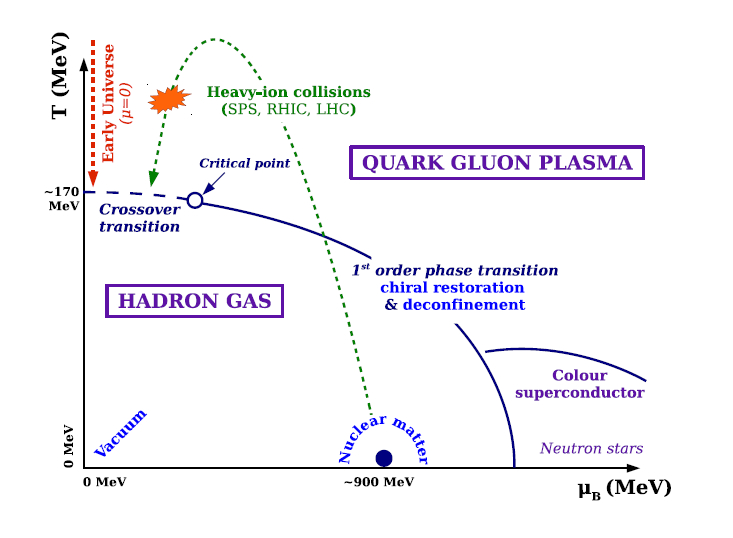
\includegraphics[width=0.8\textwidth] {FigCap1/QCDphase.jpeg}
\caption{Phase diagram of strongly interacting matter.}
\label{fig:QCDphase}
\end{figure}

Although the transformations in the early universe concerned the interactions among quarks,
this phase transition would never happened if not leaded by macroscopic
conditions, like the system temperature and density. The comprehension 
of the evolution of this state of matter 
has the promise to become accessible if we understand the thermodynamics 
laws of the QCD. It is not obvious indeed, nevertheless intriguing, 
to understand whether the QCD thermodynamics applies to the fireball 
created in the heavy-ion collisions in the laboratory, and whether the 
emitted hadrons keep a trace of the thermodynamics processes. \\

After the SPS, the Relativistic Heavy-Ion Collider (RHIC) at BNL 
has conduced experiments to create hot QCD matter through Au-Au 
collisions with the highest collision energy $\sNN = 200$ GeV per nucleon-nucleon
collision, one order of magnitude above the top of SPS energy. 
The Large Hadron Collider (LHC) at CERN is conducing experiments 
along the same line with the highest achievable center-of-mass 
energy of $\sNN = 5.02$ TeV per nucleon-nucleon collision.

\section{Micro bang vs big bang: timescales of expansion, baryonic number}
The system created in the laboratory by colliding
high-relativistic nuclei presents many similarities with 
the matter of the primordial universe, but also some differences. 
A Hubble-like expansion drives the 
evolution of the system after the collisions in the laboratory and the fireball undergoes different phases: 
\begin{itemize}
\item Pre-equilibrium phase: parton scatterings produce a large number of partons; 
they interact among each other leading the fireball to thermalize after a 
time of $\sim$ 0.6-1 fm/c;
% with the creation of high-$\pt$ probes (heavy quarks, photons) and low-$\pt$ particles;
\item QGP phase: with high-energy collisions, if the temperature inside the fireball 
exceeds the critical temperature $T_{\rm c}$, the system is in a deconfined 
phase with partonic degrees of freedom. While the phase of QGP in the early universe lasted
tens of microseconds, due to the interplay of gravity and
radiative pressure of the expanding matter, the plasma created in the laboratory 
has a lifetime of the order of 10$^{-23}$ seconds. During this time, it rapidly expands
and cools down, thus the size and local properties of
the fireball change rapidly, contrary to what happens in the 
early universe.

\item Hadronization phase: while expanding, the temperature 
of the medium drops down and, when the critical temperature $T_{\rm c}$
is reached, quarks and gluons give rise to hadrons (confinement); the hadron
gas continues the expansion and the temperature lowers further.

\item Chemical freeze-out: inelastic processes cease and the relative abundances of the various hadron species are fixed;
\item Kinetic freeze-out: even elastic collisions finish, fixing the momentum distribution of the produced particles. 
\end{itemize} 

\begin{figure}[h!]
\centering
 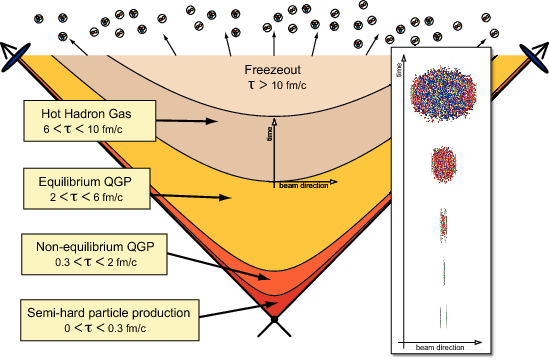
\includegraphics[width=0.8\textwidth] {FigCap1/timescales.png}
\caption{The space-time evolution of a heavy-ion collision. }
\label{fig:QCDphase}
\end{figure}


Unlike in the early universe, we expect in the laboratory a significant matter-antimatter 
asymmetry in the particle abundance, at the lower center-of-mass energies due to the
stopping of the colliding nucleons. 
At the energies of AGS and SPS, colliding nuclei tend to stop each other, forming a 
dense, baryon-rich matter and hence a system with a large $\mu_{B}$. At higher 
energies ($\sNN > 100 \Gevc$), they pass through each other leaving a nearly 
baryon-free matter in the region at central rapidity. In this case the system is closer 
to the conditions of zero baryo-chemical potential of the primordial universe. 
RICH experiments were the first to enter in the  ``baryon free'' domain. Today, ALICE, 
CMS and ATLAS, thanks to unprecedentedly high energy beams at the LHC, are 
exploring this region with even smaller baryo-chemical potential. 
Fig.~\ref{fig:YieldsVsEnergyAndronic} shows the measured yields of identified 
particles and anti-particles at mid-rapidity (rapidity being defined as 
\mbox{$y = 1/2 \; {\rm ln}((E+p_{L})/(E-p_{L}))$}, where $E$ is the particle energy 
and $p_{L}$ its momentum longitudinal to the beam direction) as a function of the 
center-of-mass energy of the collision, covering results by experiments at the 
AGS, SPS, RHIC and LHC~\cite{Andronic:2014zha}. The difference in the production 
of p and $\bar{\rm p}$ at low energies is a clear example of what discussed above. 
Because of the large stopping power in the low-$\sNN$ region, the quark content of
 the fireball is dominated by the quark content of the colliding nucleons. At LHC 
 energies, yields of particles and anti-particles are the same, 
 indicating the increasing transparency in the collision. 
The difference in the production of $\pi^+$ and $\pi^-$ at low $\sNN$ is due to the 
isospin composition of the fireball. Finally, the difference between $K^+$ and $K^-$ 
and between $\Lambda$ and $\bar{\Lambda}$ is again due to their quark content, 
$K^+ (u\bar{s})$, $K^- (\bar{u}s)$, $\Lambda (uds)$, $\bar{\Lambda} (\bar
{u}\bar{d}\bar{s})$: like in the proton case, the quark content of the colliding nucleons
drives the fireball content, whereas in regimes of large stopping power. When the collision energies become 
high enough so that the we enter the ``baryon free'' domain and particle-to-antiparticle ratios $\approx$ 1,
the baryo-chemical potential approaches $\approx 0$ values.


\begin{figure}[!t]
  \centering
  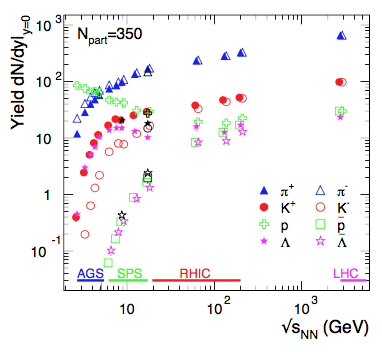
\includegraphics[width=8.5cm]{FigCap1/YieldsVsEnergyAndronic.png}
  \caption{Collision energy dependence of the multiplicities (yield, dN/dy, at mid-rapidity) of pions, kaons, protons and lambda hyperons and their antiparticles, measured in central collisions (corresponding to an average number of 350 participant nucleons in the collision) of Au or Pb nuclei~\cite{Andronic:2014zha}.}
  \label{fig:YieldsVsEnergyAndronic}
\end{figure}

% /* Expansion rates differ by 18 orders of magnitude
% Expansion in 3d, not 4d; driven by pressure gradients, not gravity
% Time scales measured in fm/c rather than billions of years
% % Distances measured in fm rather than light years
% “Heavy-Ion Standard Model” still under constructio
% Similarities: Hubble-like expansion, expansion-driven dynamical freeze-out
% chemical freeze-out (nucleo-/hadrosynthesis) before thermal freeze-out
% (CMB, hadron pT -spectra)
% initial-state quantum fluctuations imprinted on final state*/
\section{What theory tells us}
\label{sec:Lattice}
QCD is the widely accepted theory for the strong interaction. 
Phenomena at high energies, or equivalently, very short distances can be
predicted via a perturbative approach, since the coupling constant is weak. 
How the quarks are bound in the hadrons, however, is controlled by 
the large-scale behaviour of the coupling, which increases with distance. 
For such reason, Lattice Calculation is an indispensable technique. 
Lattice QCD is a non-perturbative treatment of QCD formulated 
on a discrete grid or lattice of points in space and time~\cite{Philipsen:2012nu}. 
Because of the non-perturbative nature of the theory, 
numerical simulations of Lattice QCD are the only tool 
allowing for calculations from first principles. The discretisation of the 
space-time continuum provides two main 
advantages: on one hand the problem of ultraviolet divergences typical 
of the perturbative approach is solved 
as the step of the lattice defines a shortest distance scale and hence a 
cut-off value for the momentum scale. 
On the other hand, we wish to describe a system of particles in a finite 
volume $V$, which is in thermal contact 
with a heat bath at temperature $T$. Associated with the particles, there 
may be a set of conserved charges 
$N_i$, with \textit{i}=1, 2, ... (such as the particle number, electric charge, 
baryon number etc.). In quantum field 
theory, the most direct description is in terms of the grand canonical ensemble, 
defining a density operator $\rho$ and a partition function $Z$ of the system at a temperature $T$:
\begin{equation}
\rho =e^{-\frac{1}{T}(H-\mu_iN_i)},\quad Z=Tr(e^{-\frac{1}{T}(H-\mu_iN_i)})=  \int dx \langle x|e^{-\frac{1}{T}(H-\mu_iN_i)}|x\rangle,
\end{equation}
where $\mu_i$ are the chemical potentials for the conserved charges, and 
the quantum mechanical trace is a sum over 
all energy eigenstates $|x\rangle$ of the Hamiltonian H. 
From the partition function, all other thermodynamic equilibrium quantities are 
calculable. The basic idea behind lattice 
QCD is the possibility to express the grand canonical partition function using the 
path integral representation, going in the 
domain of imaginary time. Actually, the partition function has a very similar 
formulation to the propagator of a quantum 
mechanical system between two space-time points $\langle x_b|e^{-iH(t_b-t_a)}|x_a\rangle$. 
The path integral 
formulation allows the use of Monte-Carlo methods to find the equilibrium states of the system. 
With lattice discretisation, some ``order parameters'' can be defined, which are 
sensitive to certain processes and accessible from lattice calculations. From them, 
estimates of characteristics parameters, like the critical temperature $T_c$ for the transition
to a deconfined starte, can be obtained. Among the order parameters, there are:
\begin{figure}[!t]
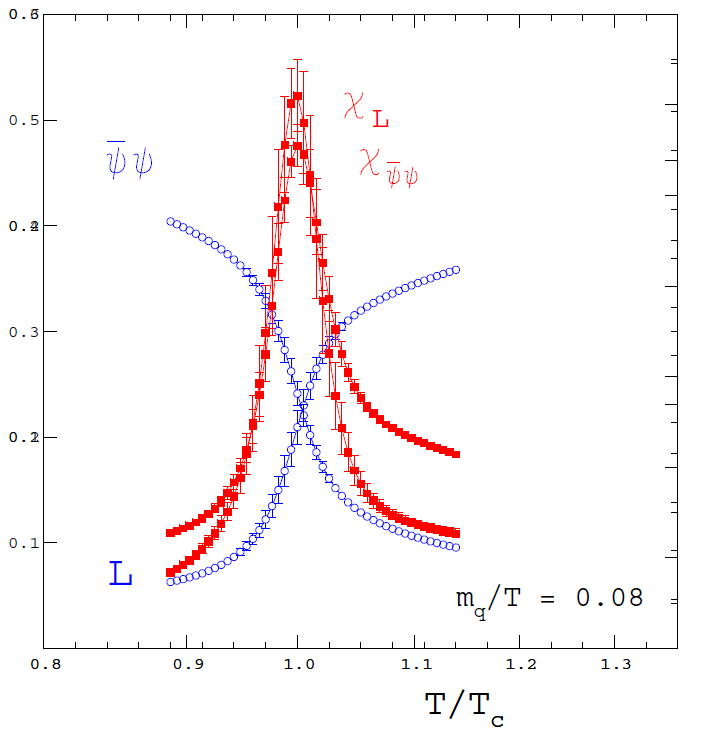
\includegraphics[width=6cm,height=6cm]{FigCap1/Lattice1.png} 
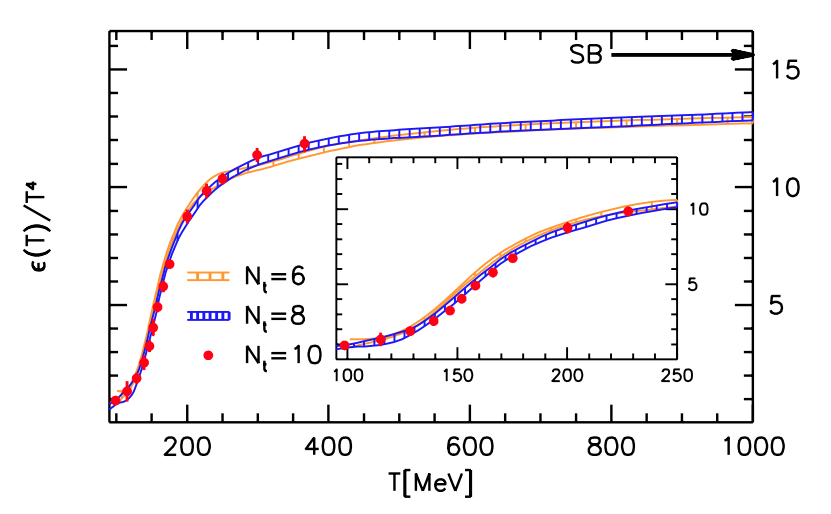
\includegraphics[width=7.5cm,height=5.8cm]{FigCap1/BW_EnDensity.png}
 \caption{(Left) Chiral condensate $\langle \bar{\psi}\psi\rangle$ and free energy function L (blue) as function of temperature. Their susceptibilities are shown in red~\cite{Karsch:2001vs}. (Right) Lattice simulation of energy density as a function of temperature. The arrows indicate the position of the Stefan-Boltzmann limit~\cite{Borsanyi:2010cj}.}
\label{fig:Lattice}
\end{figure}

\begin{itemize}
\item \textbf{Polyakov loop,} defined as:
\begin{equation}
L(T)\sim {\rm exp}\{-V(r)/T\},
\end{equation}
where $V(r)$ is the potential between a static quark-antiquark pair separated by a distance $r$. 
In pure gauge theory $V(r)\sim \sigma r$ where $\sigma$ is the string tension (two color sources 
in a confining gauge theory are bound together by a thin flux tube and this hypothesis is the
core of the effective string description of confinement~\cite{Caselle:2002vq}); hence V($\infty$) = $\infty$, 
and $L = 0$. In a deconfined medium, colour screening among the gluons leads to a melting of the 
string, which makes $V(r)$ finite at large $r$; hence $L$ does not vanish. It thus 
becomes a parameter for estimating the state of deconfinement. 
Fig.~\ref{fig:Lattice} (left) shows lattice results for $L(T)$ and the 
corresponding susceptibility $\chi_L(T)\sim \langle T^2 \rangle - \langle T \rangle ^2$. 
\item \textbf{Chiral condensate: }the effective quark mass is measured by the expectation value 
of the corresponding term in the Lagrangian, $\langle  \bar{\psi}\psi\rangle (T)$. 
The chiral symmetry is the invariance of the Lagrangian under an axial transformation of the fermion field:
\begin{equation}
\Psi \rightarrow e^{-i \gamma_{5} \frac{\vec{\tau} \cdot \vec{\theta}}{2}}\Psi
\end{equation}
where $\vec{\tau}$ are the three Pauli matrices and $\gamma_5$ 
is the chiral operator. In the limit of 
vanishing current quark masses, the Lagrangian becomes 
chirally symmetric. When confined into 
hadrons, the bare quarks ``dress'' themselves with gluons acquiring 
an effective constituent mass. 
Then, after the transition to a deconfined phase, the quarks 
would recover the "bare" mass, and the 
chiral symmetry should be approximately restored. In the calculations, 
the order parameter for the transition is the effective 
quark mass, measured as the expectation value of the corresponding 
term in the Lagrangian, that is the 
chiral condensate $\langle \overline{\psi}\psi \rangle$. In Fig.~\ref{fig:Lattice} 
(left) the behaviour of 
the order parameter as a function of temperature is shown. 
Recent results provide a measure of the critical temperature 
$T_c$ from the results for the chiral condensate, 
and it is estimated as $T_c = (154 \pm 9) $ MeV~\cite{Petreczky:2012rq}.
\item \textbf{Energy density $\epsilon$ and pressure P} at deconfinement: 
in Fig.~\ref{fig:Lattice} (right) it 
is seen that $\epsilon/T^4$ changes quickly at the critical temperature 
$T_c$, increasing from a low 
value typical of an hadron gas to a higher value closer to what expected 
for an ideal gas in the Stefan-Boltzmann limit of 
massless quarks and gluons. N$_{\rm t}$ is the number of points in the temporal
direction of a hypercubic lattice~\cite{Borsanyi:2010cj}. The 
remarkable deviation of $\epsilon/T^4$ from the
Stefan-Boltzmann limit is a clear signal of surviving
correlations in the deconfined phase.
The rapid increase in energy density is expected to occur as consequence of the increased number of degrees of 
freedom in the phase transition. %Recent calculations of Lattice QCD predicts as critical temperature $ \sim 160$ MeV~\cite{Karsch:2001vs}.

\end{itemize}


\begin{figure}[!b]
  \centering
  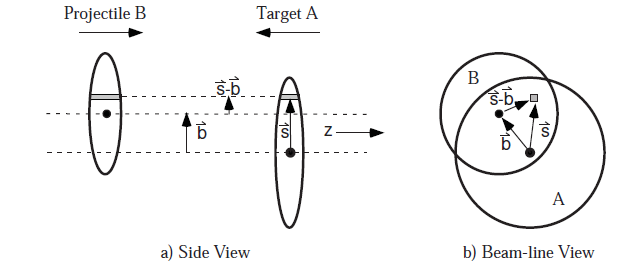
\includegraphics[width=12cm]{FigCap1/glauber.png}
  \caption{Schematic view of a nucleus-nucleus collision described in terms of the impact parameter b in the longitudinal (left) and transverse (right) plane.}
  \label{fig:image10}
\end{figure}

\section{Collision Geometry and the Glauber Model}
In a collision of two nuclei, the impact parameter \textit{b}, i.e. the distance 
between the centers of the nuclei in the transverse plane of the collision, can 
span values from 0 to about $R_1+R_2$, where  $R_1$ and  $R_2$ are the radii of 
the two nuclei if approximated with hard spheres. 
Small values of $b$ ($\lesssim$ 3.5 fm) imply central collisions. 
The impact parameter can not be measured directly, still it is 
possible to relate it to observables as the multiplicity of particles produced in the 
collision, the transverse 
energy or the number of spectator nucleons. 
The Glauber model is used to calculate the geometrical quantities that 
characterize the collision (such as the number of nucleons participating in the collisions,
the number of spectator nucleons), and that can be correlated with some
observables (such as multiplicity, transverse energy) to estimate the centrality of the
collision~\cite{Miller:2007ri}.
The model provides a phenomenological description assuming that the nucleus-nucleus 
collision can be treated as a superposition of independent nucleon-nucleon collisions.
Under the assumptions (optical limit) that, (i) at sufficiently high energies, the nucleons 
inside the nuclei are essentially undeflected after the collision, (ii) the
 nucleons are independent in the nucleus, (iii) protons and neutrons 
 are indistinguishable and (iv) the radius of the nucleus is large compared 
 to the extent of the nucleon-nucleon force, we can define the thickness 
 functions of nuclei A, B for a certain value of impact parameter $b$ (see Fig.~\ref{fig:image10}):
\begin{equation}
T_i(\vec s) = \int\,dz \rho_i(\vec s,z).
\end{equation}
The thickness function is related to the nuclear density function $\rho$. The nuclear 
density is usually parameterized by a Woods-Saxon or 3-parameter Fermi distribution:
\begin{equation}
\rho (r) = \rho_0 \frac{1+w(r/R)^2}{1+{\rm exp}(\frac{r-R}{a})},
\end{equation}
where $\rho_0$ is the nuclear density in the center of the nucleus, 
$R = (6.62 \pm 0.06)$ fm is the radius parameter of the ${}^{208}$Pb, 
$a = (0.546 \pm 0.010)$ is the skin thickness of the Pb nucleus and $w$ 
characterizes deviations from a spherical shape ($w=0$ for Pb). 
The nuclear overlap function is then defined as:
\begin{equation}
T_{AB} = \int \,d^2s T_A(\vec s)T_B(\vec s - \vec b)
\end{equation}
and it gives the probability for two incoming nucleons inside two nuclei colliding 
with impact parameter \textit{b} to be in the same elementary area $d^2s$ in the transverse plane.
By considering the mean of a binomial distribution, the average number of 
binary nucleon-nucleon collisions $\langle N_{coll}\rangle$ as a function 
of the impact parameter \textit{b} can then be written as:
\begin{equation}
\langle N_{coll}\rangle = AB \times T_{AB}(b)\; \sigma^{inel}_{NN},
\end{equation}
where $A$ and $B$ are the mass numbers of the colliding nuclei and $\sigma^{inel}_{NN}$
is the inelastic interaction cross-section of the two nucleons.
The average number of participant nucleons in the collisions (nucleons of target 
and projectile that interact) can be obtained as a function of the impact parameter $b$ as:
\begin{equation}
\begin{aligned}
N_{part} (b) &= \int A \; T_A(\vec{s}) [1- (1- \sigma_{inel} T_B(\vec{b}-\vec{s}))^B]d^2s \\
& + \int B \; T_B(\vec{b}-\vec{s}) [1- (1- \sigma_{inel} T_A(\vec{s}))^A]d^2s.
\end{aligned}
\end{equation}
The inelastic cross-section for a collision between two nuclei (A and B), 
in a certain centrality range ($0 < b < b_c$) 
can be expressed using the Glauber model geometry, as:
\begin{equation}
\label{eq:sigmaABGlauber}
\sigma_{AB}(b_c) = \int_0^{b_c} 2\pi b\,db [1 - (1 - \sigma^{inel}_{NN}T_{AB}(b))^{AB}]. %\simeq \int_0^{b_c} 2\pi b\,db \cdot AB\cdot T_{AB}(b)  \sigma^{inel}_{NN}.
\end{equation}
\begin{figure}[!t]
\centering
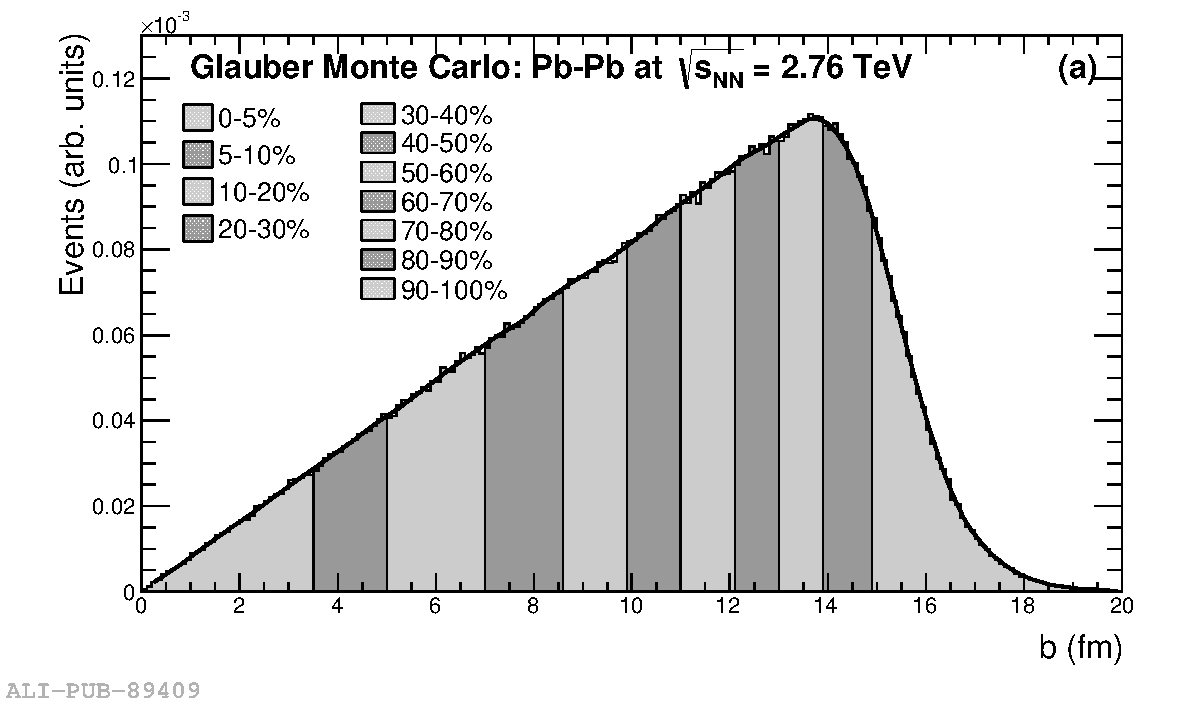
\includegraphics[width=7cm]{FigCap1/Glauberimpactpar.pdf}
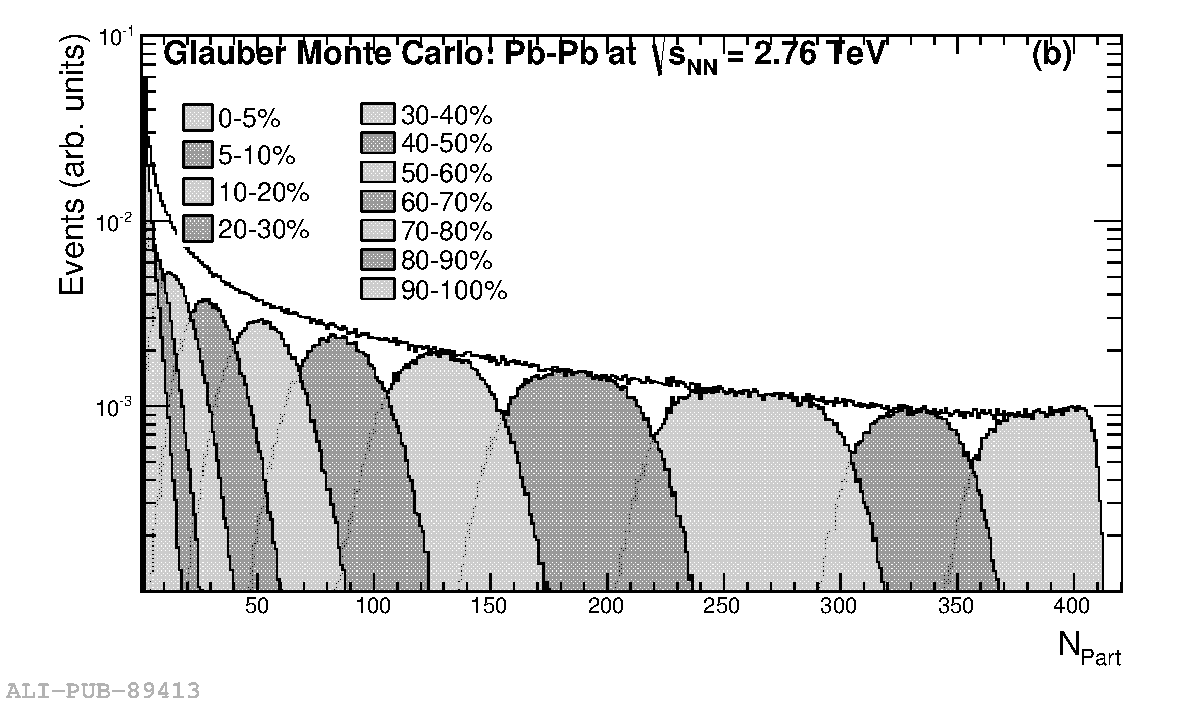
\includegraphics[width=7cm]{FigCap1/GlauberNpart.pdf}
\caption{Left: impact parameter distribution obtained from Glauber MC simulations for Pb-Pb collisions at $\sNN = 2.76$ TeV. Right: the corresponding $N_{\rm part}$ distributions for different intervals of centrality percentiles.}
\label{fig:glaubMC}
\end{figure}
The centrality is usually expressed in terms of percentiles of the total nuclear 
interaction cross section $\sigma_{AB}$ in Eq.~\ref{eq:sigmaABGlauber}.
The percentile of the cross-section for collisions in a given impact parameter
interval $b_{min}<$ b $<b_{max}$ (see Fig.~\ref{fig:glaubMC}) is given by:
\begin{equation}
c=\frac{1}{\sigma_{AB}}\int_{b_{min}}^{b_{max}} \frac{d\sigma_{AB}}{db'}db'.
\end{equation}
A simple approach to utilize the Glauber Model formulation for the
 calculation of geometry related quantities like $N_{part}$ and $N_{coll}$
is a Monte Carlo implementation. 
Furthermore, it is possible to simulate experimental quantities 
like the charged particle multiplicity and to apply similar centrality cuts as in the analysis of real data. 
In the simulation the nucleon distribution in the two colliding nuclei is randomly generated
according to their nuclear density distributions.
A random impact parameter $b$ is also associated to the collision according to the distribution
d$\sigma$/d$b \propto 2\pi b$. The nucleons travel on straight-line
trajectories and the inelastic nucleon-nucleon cross-section is assumed to be independent
of the number of collisions a nucleon underwent before. A nucleon-nucleon collision takes place if
their distance $d$ in the plane orthogonal to the beam axis satisfies:
\begin{equation}
d \leq \sqrt{\sigma^{inel}_{NN}/\pi}.
\end{equation}
Optical Glauber and MC Glauber show good agreement when calculating 
simple geometric quantities like $N_{part}$ and $N_{coll}$ as
a function of impact parameter. Some discrepancies appear at the highest impact parameters.
This is mainly due to the fact that in the Optical Approximation the incoming nucleon sees the incoming nucleus as a smooth density object and does not account for event-by-event density fluctuations.



In Chapter 3, more details will be given about the calculation 
of N\textsubscript{part} and N\textsubscript{coll} and the centrality 
determination in the ALICE experiment.


\section{Heavy-ion physics at the LHC}
Let's now turn into the experiments. The SPS program, with its several experiments, 
was mainly aimed at understanding whether a new state of matter, with the 
characteristics of a Quark-Gluon Plasma, could actually be created in the laboratory.
For a more quantitative study of the properties of this
system, we had to wait for the following research era, with the RHIC and LHC colliders.
However, the first results from the SPS revealed that Pb-Pb collisions 
were not simply a trivial superposition of elementary proton-proton (pp) collisions.
First of all, it was possible to measure quantitatively
the energy density and temperature of the fireball formed after collisions of two Pb nuclei.
A formula derived by Bjorken~\cite{Bjorken} 
revealed the energy density of the system to be around
3 GeV/fm$^{3}$, slightly above the phase transition
that the Lattice QCD predicts to be at about 0.5-0.6 GeV/fm$^3$~\cite{Hands}. At that energy density,
Lattice QCD gives a plasma temperature of about 210 MeV. The main experimental observations at the SPS 
were an abundant production of hadrons
containing strange quarks~\cite{Sandor:2004bg} (``strangeness enhancement"), 
the reduced production of the J/$\psi$ mesons~\cite{Abreu:2000ni} 
(``anomalous J/$\psi$ suppression") and the yields of 
low-mass lepton pairs~\cite{Damjanovic:2005ni} (``$\rho$ melting"). They constituted 
the signals that a new state of matter had been found.
Moreover, the NA49 experiment gave the first indications that the fireball medium 
could be described by QCD hydrodynamics, with the measurement
of the elliptic flow of pion and proton in semi-peripheral Pb-Pb collisions 
at top SPS energy~\cite{Alt:2003ab}. This observable, described in more detail 
in Sec.~\ref{sec:AnisotropicFlow}, is related with the
initial spatial anisotropy of the overlapping area of the two colliding nuclei, that is 
then converted into a final momenta anisotropy. Such a process is only possible 
if the fireball is guided by collective motion effects in a liquid-like medium with  
small viscosity. The initial results from RICH confirmed the picture 
of an extremely strongly interacting and almost perfect liquid QGP, enough opaque 
to quench any fast parton that travels througth.\\
This effect and the experimental observations mentioned before will be deeper 
explored during the LHC phase. We will go now through a revision of some of the most 
important results and open points regarding heavy-ion physics at the higher LHC energies. 

\begin{figure}[!t]
  \centering
  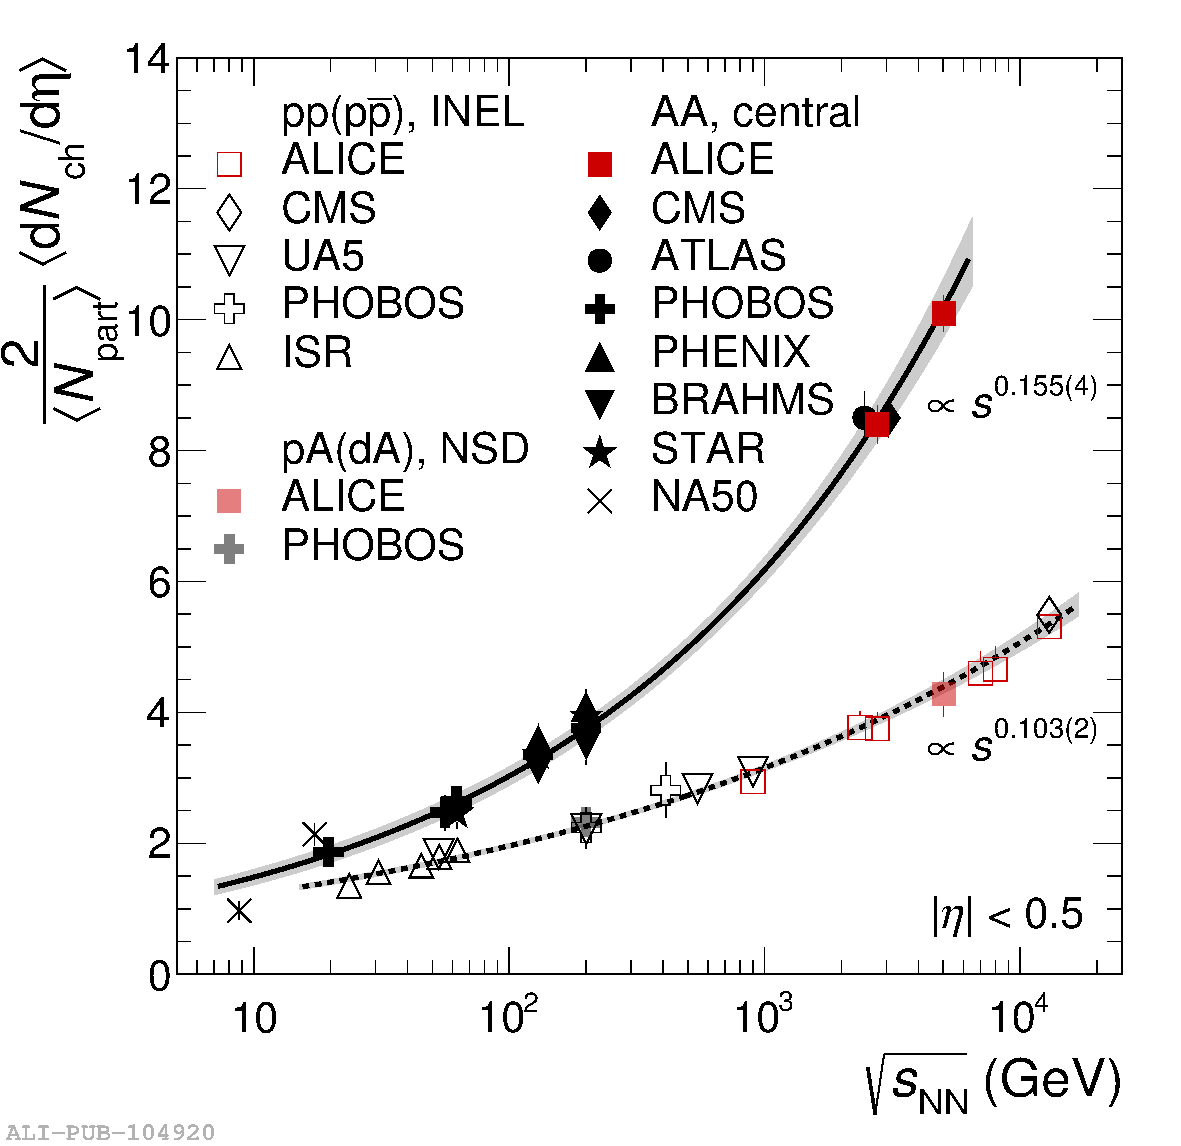
\includegraphics[width=7cm]{FigCap1/dNchdEtaVsEnergy.pdf}
  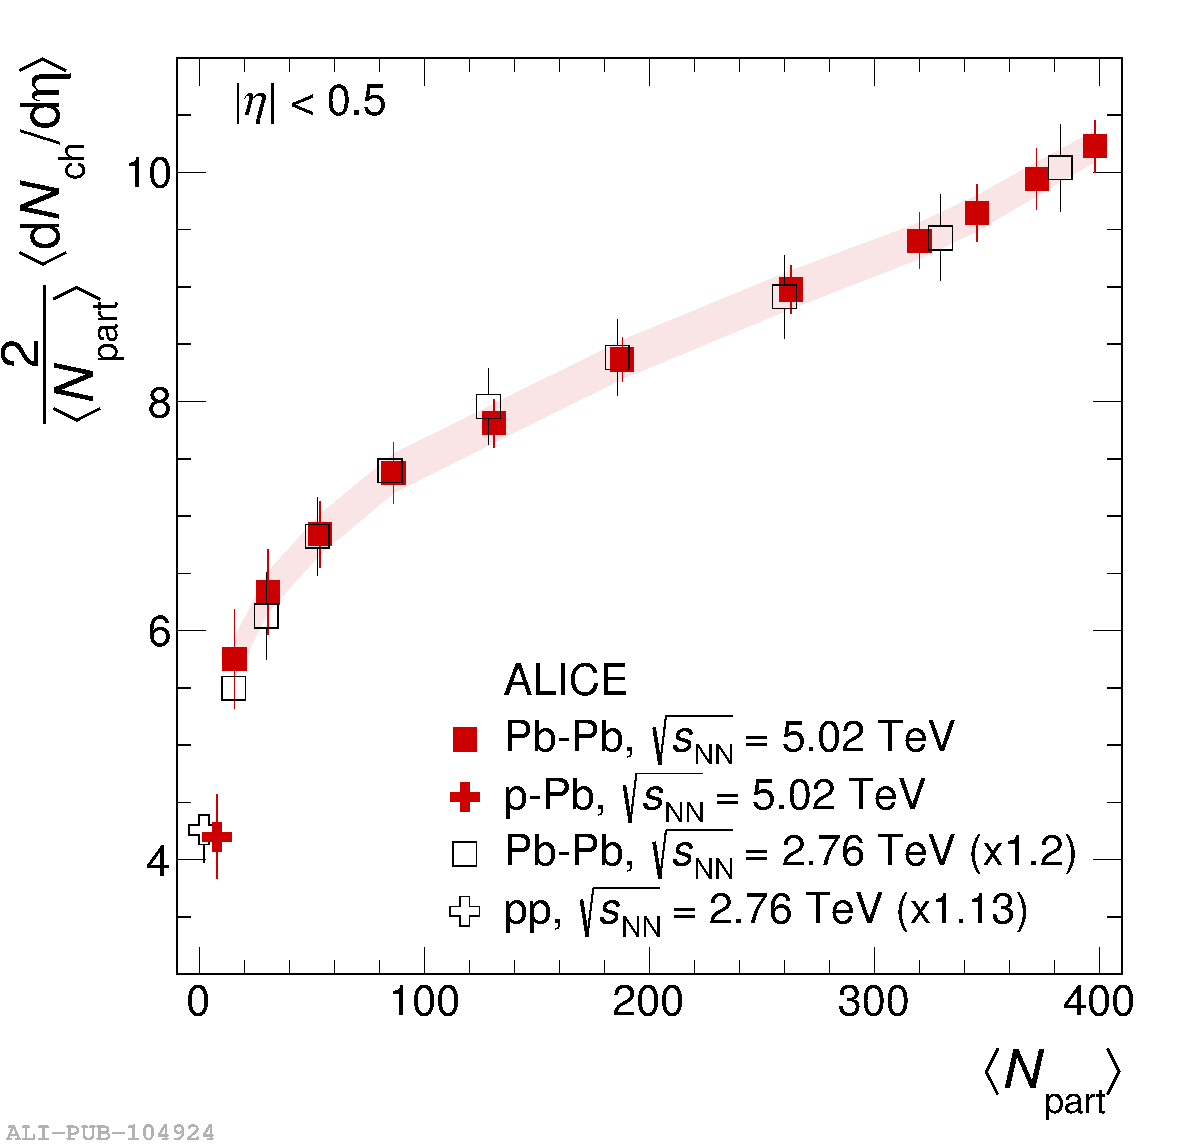
\includegraphics[width=7cm]{FigCap1/dNchdEtaVsNpart.pdf}
  \caption{(Left) Charged particle pseudo-rapidity density per participant pair for pp and central AA collisions as a function of center-of-mass energy per nucleon pair, measured in different colliding systems~\cite{Adam:2015ptt}. The fit to the power law is shown as solid (A-A) and dashed (pp) lines, together with the uncertainties on the dependence (shaded bands). (Right) Centrality dependence of (d$\Nch$/d$\eta$)/($\langle N_{\rm part} \rangle/2$) for p-Pb and Pb-Pb collisions at $\sNN=5.02$ TeV~\cite{ALICE:2012xs,Adam:2015gka}, Pb-Pb collisions at $\sNN=2.76$ TeV~\cite{Aamodt:2010cz} and pp collisions at $\sqrt{s}=7$ TeV measured with ALICE.}
  \label{fig:dNchdEta}
\end{figure}

\subsection{Particle multiplicity and energy density}
The number of particles produced in the collision (multiplicity) is related to the 
density of the created medium. Particle multiplicity depends in fact both on the 
centrality and energy of the collision. This observable is usually presented as 
a pseudo-rapidity ($\eta = - {\rm ln}(\tan(\theta/2))$ density of charged particles at 
mid-rapidity (d$\Nch$/d$\eta |_{\eta=0}$). This is useful to compare experimental 
results with different acceptances. Furthermore, particle density is usually 
divided by the average number of nucleon pairs participating to the collision 
($\langle N_{\rm part}\rangle$/2), to compare results from different 
colliding systems. The measurements by ALICE in the 5\% 
most central Pb-Pb collisions at $\sNN = 5.02$ TeV found a density of charged 
particles at mid-rapidity $\langle $d$\Nch$/d$\eta \rangle = 1943 \pm 54$ 
and, normalised per participant pair, (d$\Nch$/d$\eta$)/($\langle N_{\rm part} \rangle/2$) $ 
= 10.1 \pm 0.3$~\cite{Adam:2015ptt}.  
The left panel of Fig.~\ref{fig:dNchdEta} presents (d$\Nch$/d$\eta$)/($\langle N_{\rm part} \rangle/2$) 
as a function of the center-of-mass energy per nucleon pair. The energy dependence 
of the charged multiplicity for central heavy-ion collisions can be fitted with a power 
law of the form $as^b$, where $b = 0.155 \pm$ 0.004~\cite{Adam:2015ptt}. 
The rise is much stronger than for pp collisions where $b = 0.103 \pm 0.002$, 
obtained from a fit to the same function. It can also be noticed that the values 
of (d$\Nch$/d$\eta$)/($\langle N_{\rm part} \rangle/2$) from p-Pb collisions are included in the figure 
and lays on the pp curve, indicating that the strong rise in A-A collisions is not 
only related to the multiple interactions undergone by the participating nucleons, 
present in p-A collisions as well. The right panel of Fig.~\ref{fig:dNchdEta} 
shows the values of (d$\Nch$/d$\eta$)/($\langle N_{\rm part} \rangle/2$) 
as a function of the average number of participant nucleons 
measured by ALICE in p-Pb~\cite{ALICE:2012xs} and Pb-Pb~\cite{Adam:2015ptt} 
collisions at $\sNN = 5.02$ TeV. The Pb-Pb measurements at 
$\sNN = 2.76 $ TeV~\cite{Aamodt:2010cz} are also shown, scaled by a 
factor of 1.2 (calculated from the observed $s^{0.155}$ dependence), as 
well as the pp measurements at $\sqrt{s}= 7$ TeV~\cite{Adam:2015gka} 
scaled by a factor of 1.13. The charged particle density per participant pair 
shows a strong dependence on $\langle N_{\rm part}\rangle$, decreasing 
by a factor of about 1.8 from most central collisions to peripheral ones. The 
measurement of particle production per participant pair can be used to 
constrain models describing particle production in heavy-ion collisions 
with different mechanisms. Among the others, theoretical calculations that
 are based on gluon saturation 
 (rcBK-MC~\cite{Albacete:2011fw}, Kharzeev, Levin and Nardi~\cite{Kharzeev:2004if} 
 and Armesto, Salgado and Wiedemann~\cite{Armesto:2004ud}) can 
 give a good description of data. They are based on the idea of some 
 transverse momentum scale at which the gluon and quark phase space 
 density saturates, thus limiting the number of produced partons and, 
 hence, of particles produced in heavy-ion collisions with respect to pp collisions.  
 This results also in a centrality dependence of the multiplicity of 
 heavy-ion collisions in the models, as observed in the experimental
data. \\
The simplified Bjorken model~\cite{Bjorken:1982qr} can be used to 
estimate the initial spatial energy density from the measured 
$\langle$d$\Nch$/d$\eta$$\rangle$:
\begin{equation}
\label{Bjorken}
\epsilon_{Bj} = \frac{\langle m_T\rangle}{\tau_f A}\frac{dN_{\rm ch}}{dy}
\end{equation}
where $\tau_f$ is the formation time of the secondary particles, A is the overlap 
area of the two colliding nuclei, $\langle m_T \rangle$ is the average transverse 
mass of the created particles defined as $m_{T} = \sqrt{m^{2}+\pt^2}$ and $y$ 
is the rapidity. Starting from the measured values of d$\Nch$/d$\eta$, it is 
possible to estimate the energy density of the medium created in the collision.
At top RICH energy (200 GeV), for the most central collisions, one obtains 
$\sim 5$ GeV/fm$^3$ at the conservative estimate for the formation time 
$\tau_f$ = 1 fm/c~\cite{Bjorken:1982qr}, well above the critical value predicted 
by lattice QCD for the phase transition to QGP. For central Pb-Pb collisions at the LHC 
at $\sNN$ = 2.76 TeV the value of $\epsilon_{Bj}$ is much higher and is 
around $\sim 14$ GeV/fm$^3$~\cite{Chatrchyan:2012mb}.

\subsection{Hadron multiplicities and chemical freeze-out}
If a chemical and thermal equilibrium governs the medium when it
 undergoes chemical freeze-out, the thermal nature of the medium 
 can be expected to be imprinted in the final hadron abundances. 
 If these conditions occur, the behavior of the system at the 
 equilibrium can be described via a statistical approach, using a description 
 of the final particle yields in terms of thermodynamical quantities. 
 Following the approach described in~\cite{BraunMunzinger:2003zd}, 
 we can introduce the partition function Z($T,V,\mu_{Q}$), that 
 allows for a quantitative description of the statistical properties 
 of the equilibrated system, as a function of temperature $T$, 
 volume $V$ and chemical potentials $\mu_{Q}$. 
\begin{figure}[!ht]
  \centering
  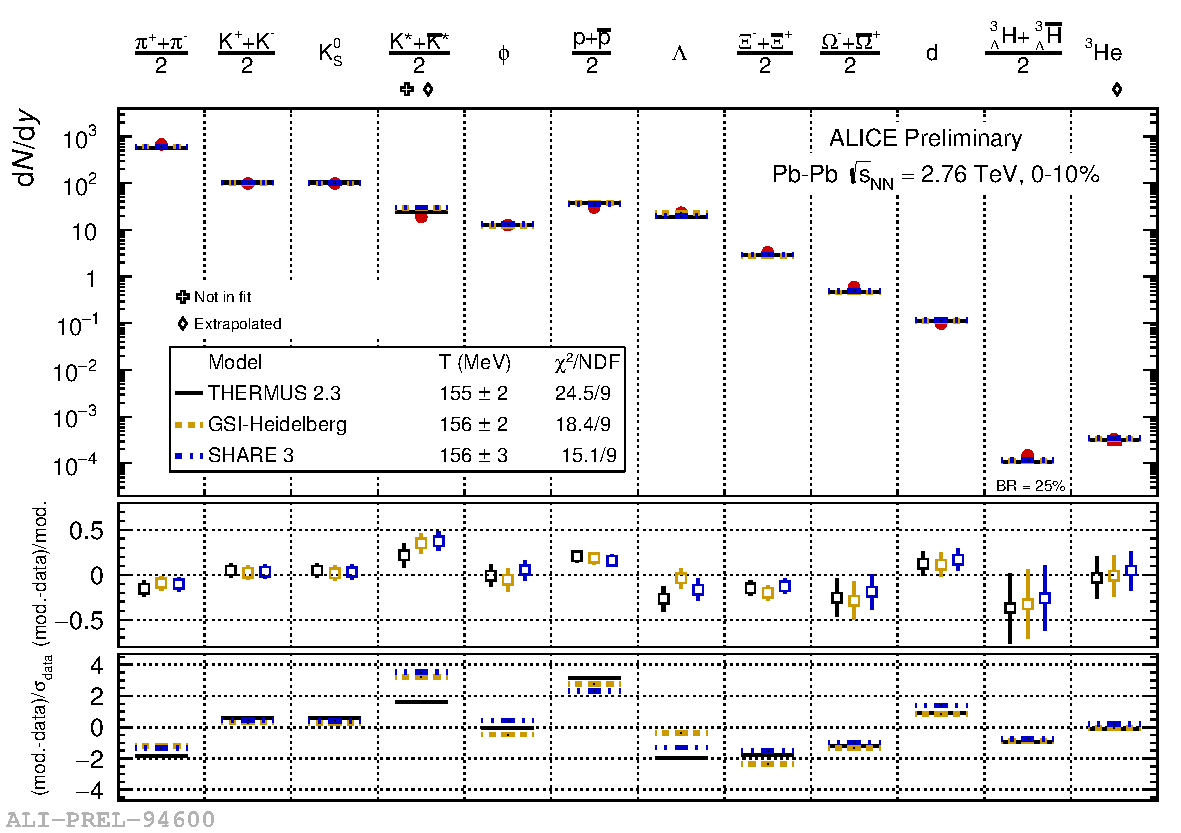
\includegraphics[width=12cm]{FigCap1/GCThermalFit_PbPb010.pdf}
  \caption{Grand Canonical thermal fit to ALICE 0-10\% Pb-Pb data at $\sqrt{s_{\rm NN}} = 2.76$ TeV~\cite{Floris:2014pta}. Excluded volume correction implemented in THERMUS and GSI with r = 0.3 fm, $\mu_{B}$ fixed to 0, $\gamma_{s}$ fixed to 1, $\gamma_{c}$ fixed to 20. }
  \label{fig:GCThermalFit_PbPb010}
\end{figure}

In the Grand Canonical (GC) ensemble, which describes a system in which 
energy and charges are on-average conserved within the full volume, the partition function is:
\begin{equation}
  \label{eq:PartitionFunction}
Z^{\rm GC} (T, V, \mu_{Q}) = {\rm Tr}[e^{-\beta(H - \sum_{i}{\mu_{Q_{i}}Q_{i}})}],
\end{equation}
where $H$ is the Hamiltonian of the system, $Q_{i}$ are the conserved charges, 
$\mu_{Q_{i}}$ are the chemical potentials needed to guarantee charges 
conservation on average in the whole system and $\beta = 1/T$ is 
the inverse temperature. At the leading order, the Hamiltonian of a non-interacting 
hadron-resonance gas contains all the degrees of freedom of a 
confined, strongly interacting medium. Further corrections can be added by 
introducing hadron repulsions, generally Van der Waals-like interactions. 
In the hadron-resonance gas a hadron mass 
spectrum containing mesons with masses below $\sim 1.5 \; \Gevcc$ and 
baryons with masses below $\sim 2\; \Gevcc$ is considered. In this mass interval, the 
hadronic spectrum is well known as well as the decay channels of resonances 
and particles. With these assumptions, the maximum temperature for which
 the model can be considered trustable is $\sim 200$ MeV. The GC partition 
 function of a non-interacting system, like that of our hypothesis, is given by 
 the product of the independent partition functions of all the hadronic species. 
 In the logarithmic form we write:
\begin{equation}
  \label{eq:LnPartFunction}
{\rm ln} Z(T, V \vec{\mu}) = \sum_{i} {\rm ln} Z_{i} (T, V, \vec{\mu}),
\end{equation}
where $\vec{\mu} = (\mu_B, \mu_S, \mu_Q)$ are the chemical potentials 
related to the baryon number, strangeness and 
electric charge, and the sum is over all hadron species $i$.
The density of particles of species $i$ can be obtained from Eq.~\ref{eq:LnPartFunction} as:
\begin{equation}
\label{eq:ParticleDensity}
n_{i} (T, \vec{\mu}) = \frac{\langle N_{i} \rangle}{V} = \frac{1}{V}\frac{\partial (T {\rm ln}Z_i^{GC})}{\partial \mu_i} = \frac{T g_{i}}{2\pi^{2}} \sum_{k=1}^{\infty} \frac{(\pm 1)^{k+1}}{k} \lambda_{i}^{k} m_{i}^{2}K_{2}(\frac{km_{i}}{T}),
\end{equation}
where (+) is for fermions and (-) for bosons, $g_{i}$ is the spin-isospin 
degeneracy factor, $\lambda_{i} = e^{Q_{i}\mu_{i}}$ is the fugacity 
term and finally $K_{2}$ is the modified Bessel function.
Further corrections to the particle density are necessary at high 
temperature ($\gtrsim 100 $ MeV) or density, where the contribution 
to the particle yield $N_{i}$ from resonance decays becomes 
dominant with respect to the thermal production of the species. 
Other deviations from the GC description can be taken into 
account by introducing parameters for strange, charm or 
light quarks ($\gamma_{S}, \gamma_{C}$ and $\gamma_{q}$) 
production. For example, in case there is no thermalisation for 
the strangeness component in the medium, a factor 
$\gamma_{s}<1$ is needed, usually whenever the size of system 
is small (i.e. pp collisions) or at low collision energies. 
The usage of $\gamma_{q}$ is only applied in the so called 
non-equilibrium model SHARE~\cite{Petran:2013lja}. This model 
describes an expanding, super-cooled quark-gluon plasma which 
undergoes a sudden hadronization without further re-interactions.
Among the five parameters of Eq.~\ref{eq:ParticleDensity} 
($T, V, \mu_B, \mu_S, \mu_Q$), up to three can be fixed with
 the knowledge of the conditions of the initial state. 
 The other two parameters can be obtained by fitting the measured
  particle yields. In Fig.~\ref{fig:GCThermalFit_PbPb010}, a 
  Grand-Canonical thermal fit with three different models using 
  T and V as free parameters is performed on the $y$-differential 
  identified particle yields measured by ALICE in the 10\% most 
  central Pb-Pb collisions at $\sqrt{s_{\rm NN}} = 2.76$ TeV~\cite{Floris:2014pta}. 
  The fit quality is not fully satisfactory ($\chi^{2}/ndf \sim 2$), 
  while it used to be of order 1 for RHIC energies~\cite{Andronic:2008gu}. 
  The temperature, as parameter of the fit, results to be of the order of 155 MeV. 
The measured p and $\Xi$ yields have a bad agreement with the fit 
(2.5 $\sigma$ and 2 $\sigma$ respectively). The measurements of resonances 
in central Pb-Pb collisions suggest elastic re-scattering in the late 
hadronic phases, that becomes quite important for pion production. 
If protons are excluded from the fits, the fit quality improves and the 
temperature goes up to $\sim$160 MeV (closer to RHIC results). 
Non-equilibrium models like SHARE describe most hadrons very 
nicely but overestimate the nuclei by almost an order of magnitude, 
while the equilibrium model predicts them very nicely. An other possible
interpretation is that inelastic processes during the hadronic phase may
not be completely negligible, rather affecting baryon production. In 
particular, baryon annihilation in the hadronic phase should lead
to a reduction of the proton yields~\cite{Becattini:2014hla,Becattini:2012xb}. Other models 
suggest that a single freeze-out temperature is not enough to describe
 the data~\cite{Bellwied:2013cta}, but temperature for lighter and heavier
  quarks could be different. So far, the production mechanism is not yet 
  clearly understood as well as how the temperature from the thermal 
  fit relates to the QCD phase transition temperature.
  
\subsection{Strangeness enhancement}
\label{subsec:StrangEnhancSPS}
The original idea of enhanced production of hadrons containing strange quarks 
as a signature of the quark deconfinement was proposed in 1980 by Rafelski 
and Hagedorn \cite{PhysRevLett.48.1066},\cite{Muller:2011tu}. As there are no 
strange quarks in the colliding nuclei, it follows that all strangeness must be 
created in the collision or in the QGP phase. Strange quarks are hard to 
produce at temperatures below $T_c$ since their effective mass is larger 
than $T_c$ when chiral symmetry is broken, but easy to produce at temperatures 
above $T_c$ since the current mass of the strange quark is $m_s \sim 100$ MeV/$c^2$, 
due to chiral symmetry restoration (see Sec.~\ref{sec:Lattice}). 
\begin{figure}[!ht]
  \centering
  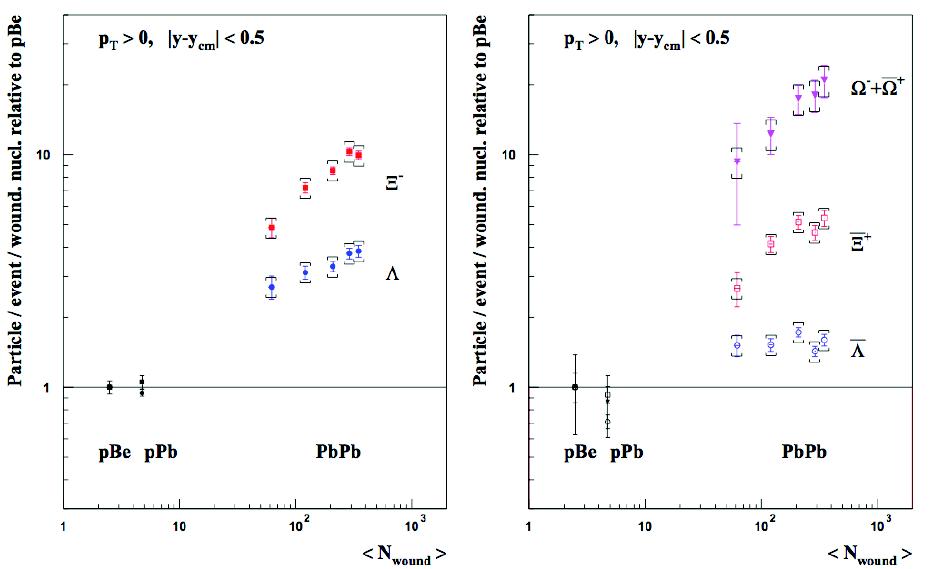
\includegraphics[width=12cm]{FigCap1/strangEnhancSPS.png}
  \caption{ Hyperon enhancement as a function of the number of the wounded nucleons measured by the NA57 experiment in Pb-Pb collisions at $\sNN = 17.2$ GeV~\cite{Sandor:2004bg}.}
  \label{fig:sEnhancSPS}
\end{figure}
For $T > T_c$, also \textit{u} and \textit{d} quark masses 
decreases to $m_q \sim 0$ MeV/$c^2$, but the 
strange quark production becomes important. In a simple hadron gas, 
even if it is possible to produce strange particles from some inelastic 
scattering such as $\pi^0+p \rightarrow K^++\Lambda$, it is less probable 
to produce multi-strange baryons, like $\Xi ^-$ and $\Omega$, as 
they are the result of more than one consecutive reactions. In presence 
of QGP, instead, it is expected an enhancement in the production of 
multi-strange baryons relative to pp reactions of about one order of magnitude.
The abundant strangeness production in QGP is due to the large gluon 
density of the system, which favours gluon-fusion processes
$gg \rightarrow s\bar{s}$. 
The Grand Canonical (GC) formulation is used whenever the conservation law of
a quantum number, for example strangeness, can be on average implemented by using
the corresponding chemical potential. This approach can be used in systems 
with a large number of produced particles. For smaller systems like pp or pA
collisions, this is no longer valid and the Canonical (C) formulation must be used
in turn. The canonical conservation of quantum numbers strictly reduces the phase
space available for particle production~\cite{Beutler:2009cc}, and this is usually referred to as canonical suppression~\cite{Tounsi:2001ck}.
This is the essence of the strangeness enhancement from pp to AA collisions.\\
In experiments the magnitude of strangeness production is usually estimated by measuring 
the enhancement factor, defined as the ratio of the yields of a given particle 
specie per participant nucleon in nucleus-nucleus collisions over the same 
ratio measured in smaller system (pp or pA). The first evidence of 
strangeness enhancement was measured by the NA57 and WA97 
collaborations~\cite{Sandor:2004bg} in fixed-target Pb-Pb collisions at 
$\sqrt{s_{NN}}$= 17.2 GeV. The enhancement factor measured by NA57 
is shown in Fig.~\ref{fig:sEnhancSPS} for $\Lambda$, $\Xi^-$ (left) and 
their anti-particles (right) in p-Pb, p-Be and Pb-Pb collisions as a function 
of the number of participating nucleons. It is observed a hierarchy for these 
enhancement factors in Pb-Pb collisions, depending on the strangeness
 content of the particles and also on the collision centrality. In p-Be and in 
 p-p there is no evidence of strangeness enhancement. 

\subsection{Collective flow and kinetic freeze-out}
The Flow is a collective phenomenon, which is observed as a collective 
motion pattern superimposed to the chaotic thermal motion of the 
particles inside the fireball. Its origin is related to the large pressure gradients 
generated when compressing and heating nuclear matter. It is possible 
to distinguish between different types of flow. In the following, 
the radial and the anisotropic flow in the transverse plane are discussed. 

\subsubsection{Radial flow}
\label{sec:RadialFlow}
For what concerns the particle production in pp collisions, 
following the approach in~\cite{Schnedermann:1993ws} we 
can treat the invariant yield of low $\pt$ particles of a given species as radiated by a
 thermal source with temperature $T$:
\begin{equation}
\label{eq:ThermalSource}
E\frac{d^{3}n}{d^3p} = \frac{dn}{dy \; m_{T} dm_T\;d\varphi} = \frac{gV}{(2\pi)^3}E\;e^{-(E-\mu)/T},
\end{equation}
  where $g$ is the spin-isospin degeneracy factor for the considered particle 
  species, $\mu$ is the grand canonical potential $\mu = n\mu_{B}+ s\mu_S$, 
  originating from the quantum numbers $n$ and $s$ for baryon and 
  strangeness content, $y$ is the rapidity, $m_{T}$ the transverse 
  mass and $\hbar = c = k_B = 1$. By integrating Eq.~\ref{eq:ThermalSource}
   over rapidity using the modified Bessel function $K_1$, we obtain
    the transverse mass distribution $dn/(m_Tdm_T)$, which behaves 
    asymptotically like a decreasing exponential for transverse masses 
    larger than the source temperature: 
\begin{equation}
\label{eq:SpectraBZ}
\frac{dN}{m_T dm_T} = \frac{V}{2\pi^2} m_T K_1 (\frac{m_T}{T}) \xrightarrow{m_T \gg T} V^\prime \sqrt{m_T} e^{-m_T/T}.
\end{equation}
It has been experimentally verified in pp collisions the universality, at low $\pt$,
of the temperature $T$ of the exponential slope of Eq.~\ref{eq:SpectraBZ}. 
In the low-$\pt$ region ($\lesssim 1 \, \Gevc$), indeed, particles originate from soft processes
and their production is governed by a Boltzmann exponential distribution. 
This law does not anymore describe production at higher $\pt$, where hard processes
govern particle emission and the production spectra result better reproduced by power law functions.
 The physical interpretation of $T_{slope}$ is the temperature of the particle
 emitting source. The universality of $T_{slope}$ for different 
 particle species is commonly referred to as $m_{T}$-scaling. When 
 moving to nucleus-nucleus collisions, a breaking of the $m_T$-scaling 
 occurs at low $\pt$ and the slopes of the spectra are observed to 
 decrease with increasing particle mass~\cite{Appelshauser:1998yb,Arnaldi:2007ru}.
  The effect is present at all centralities, but it is stronger for central
   collisions. The slope of the exponential law, at low $\pt$, can be expressed as:
\begin{equation}
\label{eq:Tslope}
T_{slope} = T_{fo} + \frac{1}{2}m \beta_{\rm T}^{2},
\end{equation}
where the second term accounts for the dependence on the mass 
and the velocity is related to the radial flow, i.e. the collective velocity
 arising from the expansion of the fireball. The first term still accounts
  for the Brownian motion of the particles, present in Eq.~\ref{eq:SpectraBZ}.
   This is the idea developed within the Boltzmann-Gibbs blast-wave 
   model~\cite{Schnedermann:1993ws}, where the radial expansion 
   velocity distribution $\beta_{\rm T}(r)$ in the region \mbox{$0 \leq r \leq R$} 
   is parametrized by relating it to the surface velocity $\beta_s$ via:
\begin{equation}
\label{eq:Br}
\beta_{\rm T} (r) = \beta_s \Big(\frac{r}{R}\Big )^n,
\end{equation}
where the exponent $n$ is used to tune the shape of the spectra profile.
\begin{figure}[!t]
  \centering
%   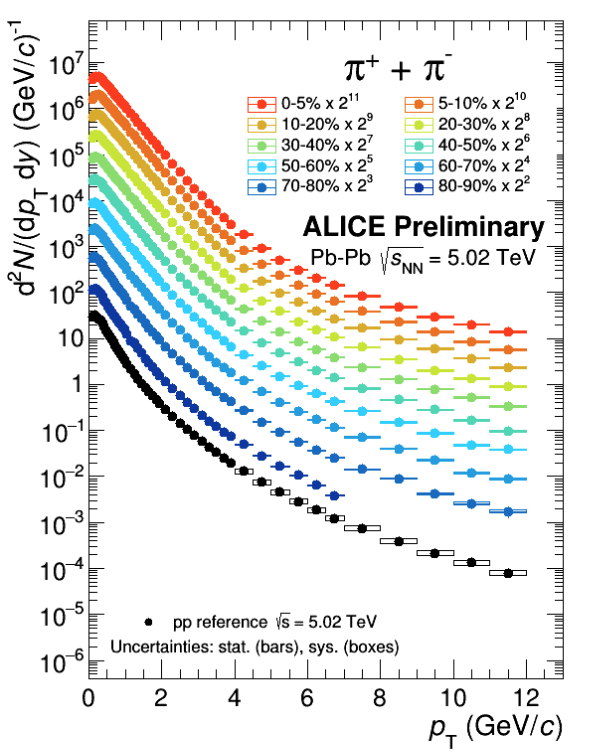
\includegraphics[height=7cm]{FigCap1/PionsPbPb5TeV.png}
   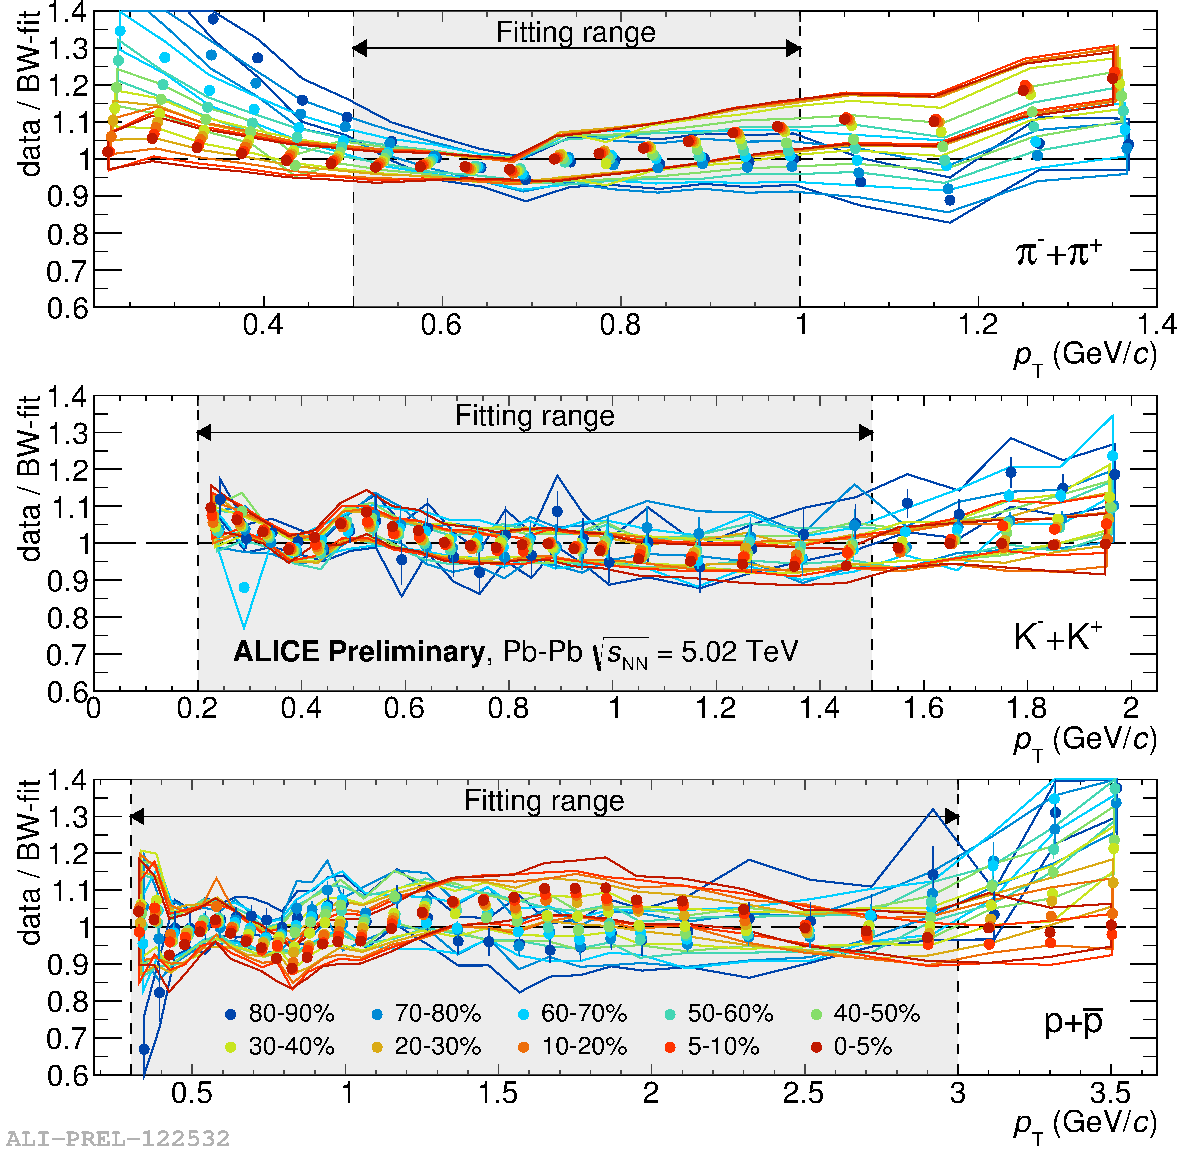
\includegraphics[height=8cm]{FigCap1/BW_5TeV.pdf}
 \caption{Ratio data to blast-wave fit for $\pi, k, p$ spectra as a function of $\pt$ in different centrality classes in Pb-Pb collisions at $\sNN = $ 5.02 TeV~\cite{Jacazio:2017dvy}, measured by ALICE.}
  \label{fig:BWfit}
\end{figure}
\begin{figure}[!t]
  \centering
  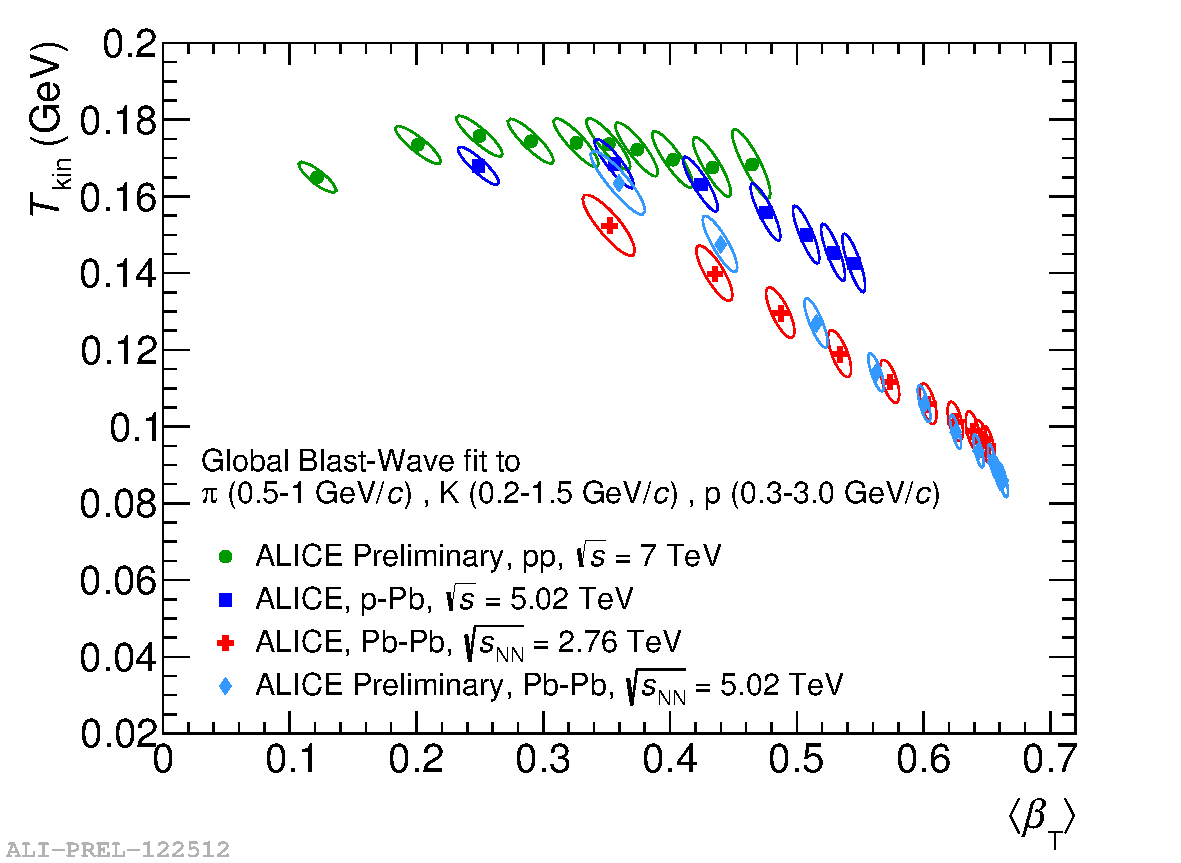
\includegraphics[height=6cm]{FigCap1/BWfit_BetaTplot.pdf}
 \caption{$T_{kin}$ vs $\langle \beta_T \rangle$ from blast-wave fits for different colliding systems and energies~\cite{Jacazio:2017dvy}.}
  \label{fig:BetaTplot}
\end{figure}

The observed particle spectrum results from the sum 
of the spectra of individual thermal sources each boosted with the 
boost angle $\rho = \tanh^{-1}(\beta_{\rm T})$:
\begin{equation}
\label{eq:BlastWave}
\frac{dN}{\pt d\pt d\phi dy}\propto \int_{0}^{R} r dr\;  m_{T}\;  K_{1} \; (\frac{m_{T} \cosh(\rho(r))}{T_{fo}})\;  I_{0}\; (\frac{\pt \sinh(\rho(r))}{T_{fo}}).
\end{equation}
It is a three parameter ($T_{fo}, \beta_s, n$) simplified hydrodynamical model.
The blast-wave fit to the measured spectra allows
  an estimate of the kinetic freeze-out temperature $T_{fo}$ and 
  radial velocity $\beta_{\rm T}$. An example of data to blast-wave fit for the 
  measured spectra of pions, kaons and protons in Pb-Pb collisions at $\sNN = $ 5.02 TeV 
   by ALICE is shown in Fig.~\ref{fig:BWfit}, as a function of $\pt$ (different centrality classes 
   are in different colours).
  
Fig.~\ref{fig:BetaTplot} shows the ALICE results 
for the blast-wave parameters for different colliding systems and energies. Blast-wave parameters
  in Pb-Pb collisions at $\sNN = 5.02$ TeV follow the trends with collision centrality observed at
   lower energy ($\sNN = 2.76$ TeV). The largest expansion velocity 
   is for central Pb-Pb collisions, as well as the lowest temperature
    for the kinetic freeze-out.\\

\subsubsection{Anisotropic flow}
\label{sec:AnisotropicFlow}
The anisotropic flow is characteristic of non-central collisions, where the 
finite impact parameter creates a fireball with a geometrical anisotropy. 
Due to particle rescatterings during the system evolution, the initial spatial 
anisotropy is transferred to a final state momentum-space anisotropy. No
 rescatterings during the system evolution or any delays in time of such 
 interactions would lead to no momentum anisotropy in the final state or
  to a decrease in the elliptic flow signal. Hence, the characterization of 
  anisotropic flow is important as it is sensitive to particle interactions very 
  early in the system evolution. Informations of medium properties, such as Equation of 
  State, sound velocity or shear viscosity can be exctracted by a comparison 
  of the measured anisotropic flow and hydrodynamic model calculations.
\begin{figure}[!ht]
  \centering
  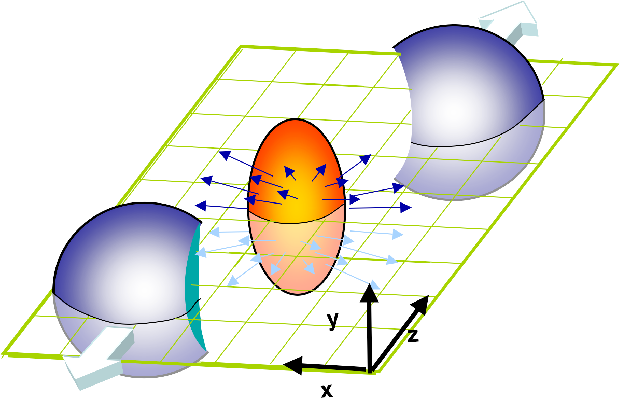
\includegraphics[width=8cm]{FigCap1/elliptic_flow_3D_medium.png}
  \caption{Picture of a semi-peripheral collisions and the pressure gradients arising from a geometrical anisotropy.}
  \label{fig:elliptic_flow_3D_medium}
\end{figure}
In non-central heavy-ion collisions, an almond-shaped interaction 
volume is created (see Fig.~\ref{fig:elliptic_flow_3D_medium}).
The reaction plane is defined by the impact parameter itself and the 
beam line (xz plane in Fig.~\ref{fig:elliptic_flow_3D_medium}). 
A larger pressure gradient in the
 reaction plane than perpendicular to it is expected. This generates an
  anisotropy in azimuthal distributions of the particle momenta with 
  respect to the reaction plane, which can be detected in the measured
   particle azimuthal distributions. This distribution can be parametrized 
   through a Fourier series decomposition:
\begin{equation}
\label{eq:FourierAzimuthExpansion}
E \frac{d^3N}{d^3p} = \frac{1}{2\pi} \frac{d^2N}{\pt d\pt dy} (1 + \sum_{n=1}^\infty 2v_n {\rm cos} (n(\varphi - \Psi_r))),
\end{equation}
where $\varphi$ is the azimuthal direction of the emitted particle and 
$\Psi_r$ denotes the (true) reaction plane angle.
In the formula, {\it v$_n$} are the Fourier coefficients, and they can be 
evaluated as $v_n = \langle cos(n(\varphi - \Psi_r)) \rangle$, where 
$\langle \rangle$ indicates an average over all particles in all events with
 their azimuthal angle $\varphi$ in a given rapidity and $\pt$ momentum at
  a fixed centrality. The sine terms vanish due to the reflection simmetry 
  with respect to the reaction plane. {\it Direct} and {\it elliptic flow} 
  are common terms for the first and the
second order Fourier coefficients respectively in the particle azimuthal 
distribution in Eq.~\ref{eq:FourierAzimuthExpansion}, but coefficients 
up to at least 6th order were measured at the LHC~\cite{ATLAS:2012at}.
With the large amount of data provided by the LHC, in fact, it became accessible
to study not only the on-average anisotropies but the initial space geometries 
fluctuations~\cite{Aad:2013xma,Schukraft:2012ah}, to which first-order and higher-order Fourier 
coefficients were indeed found to be sensitive. 
The positions of the nucleons in the overlap region of the colliding nuclei 
can fluctuate to create matter distributions dipole (n = 1) and
sextupole (n = 3) asymmetries~\cite{Teaney:2010vd,Alver:2010dn,Alver:2010gr}, which are converted into 
non-zero first-order and higher-order harmonic coefficients. 
Fig.~\ref{fig:vnHydro} shows
   comparison to viscous hydrodynamics calculations~\cite{Gale:2012rq} of the 
   Fourier coefficients $v_n$ up to 5$th$ order measured by ATLAS~\cite{ATLAS:2012at}
    (left panel) in Pb-Pb collisions at $\sNN = 2.76$ TeV and 
    PHENIX~\cite{Adare:2011tg} and STAR~\cite{Pandit:2012mq} 
    (right panel) in Au-Au collisions at $\sNN = 200 $ GeV. The value
     of the shear viscosity $\eta/s$ of the medium that allows a good parametrization 
     of hydro calculations for Au-Au collisions at top of RICH energy is 0.12, while the value
      for Pb-Pb collisions at the LHC at $\sNN = 2.76$ TeV is 0.2. 
      This reveals a dependence of the shear viscosity on the temperature of the system.
\begin{figure}[!ht]
  \centering
  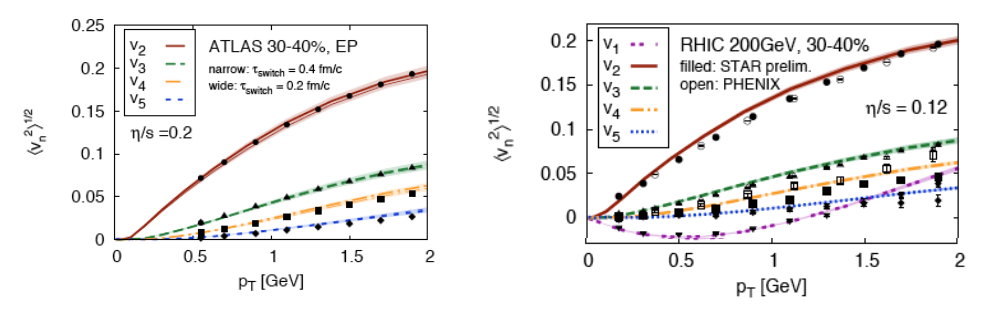
\includegraphics[width=15cm]{FigCap1/RICH_ATLAS_vn.png}
  \caption{Fourier components of anisotropic transverse flow, $v_n(\pt)$, for Pb-Pb collisions at the LHC (left panel) and for Au-Au collisions at RICH (right panel), in comparison with viscous hydrodynamics calculations~\cite{Gale:2012rq}.}
  \label{fig:vnHydro}
\end{figure}
\begin{figure}[!ht]
  \centering
  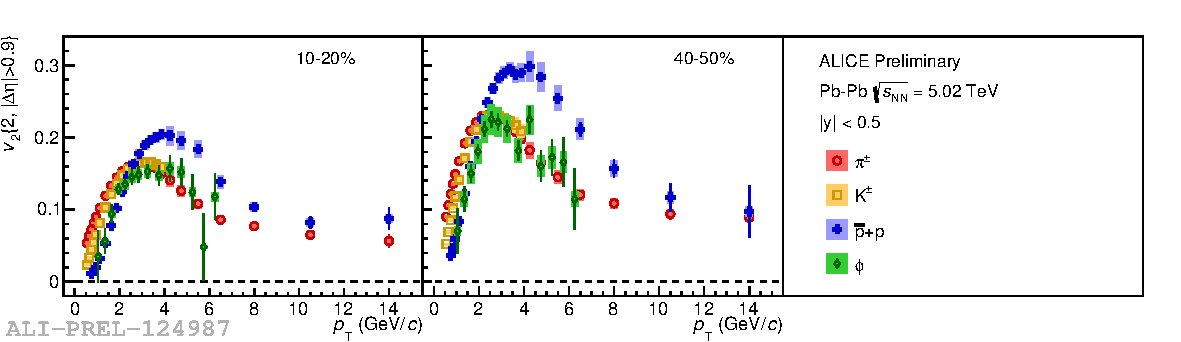
\includegraphics[width=15cm]{FigCap1/v2IdentifiedParticles.pdf}
  \caption{Elliptic flow coefficient $v_2$ of $\pi^{\pm}, K^{\pm}, p(\bar{p})$ and $\Phi$ meson for 10-20\% (left) and 40-50\% (right)
collision centrality as function of $\pt$~\cite{Bertens:2017krr}. Statistical uncertainties are shown as bars and systematic uncertainties as boxes.}
  \label{fig:v2IdentifiedParticles}
\end{figure}
Fig.~\ref{fig:v2IdentifiedParticles} shows the $\pt$-differential 
$v_2$ of $\pi^{\pm}, K^{\pm}, p(\bar{p})$ and $\Phi$ mesons for 10-20\% (left)
and 40-50\% (right) collision centrality~\cite{Bertens:2017krr}, measured by 
ALICE~\cite{Bertens:2017krr} in Pb-Pb collisions at $\sNN = 5.02$ TeV.
For $\pt < 2$ $\Gevc$, one can notice that the $v_2$ of the different species
 follows a mass ordering, which is expected for a hydrodynamically expanding 
 source and is indicative of collective radial flow.
For 3 $< \pt < 8$ $\Gevc$, particles are grouped according to their valence
 quarks, which supports the
hypothesis of particle production via quark coalescence~\cite{Molnar:2003ff}. 
The non-zero $v_2$ at high $\pt$ is attributed to path-length dependent 
in-medium energy loss which is discussed in the next section~\cite{Gyulassy:2000gk}. The $\Phi$ meson, 
with its mass close to proton mass, is a very good probe of quark scaling and 
mass ordering. Indeed, the $\Phi$-meson $v_2$ follows proton $v_2$ at low 
$\pt$, but pion $v_2$ at intermediate $\pt$. \\

\label{sec:ChiralSymm}
\begin{figure}[!ht]
  \centering
  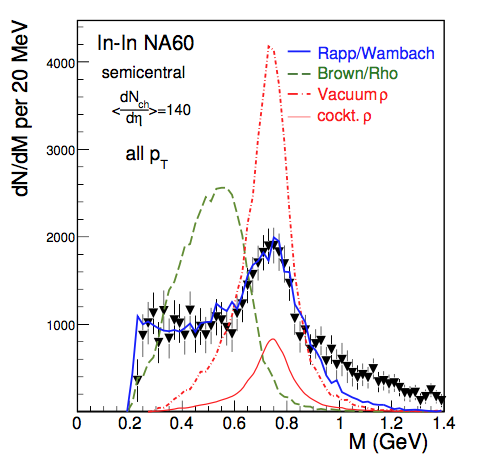
\includegraphics[width=7.2cm]{FigCap1/rhoMelting.png}
  \caption{Di-muon pair invariant mass distribution after 
background subtraction to the $\rho$ meson peak, for In-In collisions at d$N_{ch}$/d$\eta$ = 140, compared to model predictions~\cite{Rapp:2012zq}.}
  \label{fig:JPsiSuppressionNA50}
\end{figure}
\subsection{Chiral symmetry restoration}
If, on one side, chiral symmetry restoration should play a role in the 
observed strangeness enhancement (see Sec.~\ref{subsec:StrangEnhancSPS}),
on the other hand, signatures of this effect could also be found in the line shape of the
invariant mass distribution of thermal low-mass ($< 1$ GeV) dileptons.
Their production is in fact largely carried by light 
vector mesons $\rho, \omega$ and $\phi$. For this reason their are ideal to investigate
changes in the vector-meson mass distributions as the critical temperature for chiral
restoration is approached and surpassed. Changes both in width and in mass of
the mesons were originally advocated as signatures of the chiral transition~\cite{Pisarski:1981mq}. 
Among light vector mesons, the $\rho$ meson was used from the very beginning as the test particle for in-medium 
modifications, due to the abundant production
of $\pi^+ \pi^- \rightarrow \rho$ and subsequent decay $\rho \rightarrow \mu^+ \mu^- $ 
with a lifetime of 1.3 fm/c, shorter than the time between hadronization and the thermal freeze-out. 
Fig.~\ref{fig:JPsiSuppressionNA50} (right) shows NA60 measurement of the 
low-mass di-muon pair invariant mass distribution after 
subtracting the background to the $\rho$ meson peak, 
measured in In-In collisions at top SPS energy~\cite{Damjanovic:2005ni}. The $\rho$ meson is
clearly broadened in the medium as compared to the vacuum case, 
while no sign of mass shift is observed. The measurement
was found to be in good agreement with models describing an in-medium broadening 
scenario (Rapp/Wambach~\cite{Rapp:2012zq}).

\subsection{Jet quenching}
\label{sec:JetQuenching}
Partons produced in the hard scattering processes occurring in the early stages of the 
collisions fragment into collimated cascades of hadrons, that are called jets. 
In heavy-ion collisions partons propagate inside the hot and dense QGP,
 and lose energy because of interactions with the colored medium 
 (jet quenching), primarily via gluon radiation and, to smaller extent, 
 elastic scattering~\cite{Qin:2015srf}. The energy loss ($\Delta E$) carries 
 important information about transport coefficients 
 of the QGP (different for radiative or collisional processes), because it
  is expected to be dependent on the opacity 
 (associated to the medium density and the interaction strength) 
 and on the path length $L$ traversed by the parton inside the medium.
  Different models predict linear and quadratic dependences on $L$ 
  of the energy loss for elastic~\cite{Thoma:1990fm} and radiative~\cite{Baier:1996sk} 
  collisions respectively (a cubic dependence is predicted within the 
  AdS/CFT framework). Furthermore, $\Delta E$ also depends on the 
  color charge (different for quarks and gluons) and on the quark mass, 
  as it will be discussed in Sec.~\ref{sec:HFEnLossinAA} focusing in more detail on the heavy flavour quarks.

\begin{figure}[!ht]
  \centering
  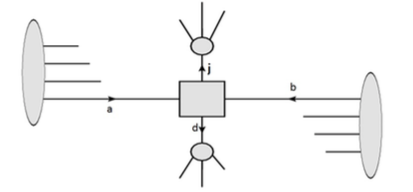
\includegraphics[width=10cm]{FigCap1/Scattering.png}
  \caption{Schematic illustration of high $\pt$ hadron production in high-energy nuclear collisions. }
  \label{fig:Scattering}
\end{figure}

In perturbative QCD, the production cross-section for a hadron $h$ 
from a process involving high-momentum transfer can be described 
using a factorisation approach as a convolution of the incoming parton distribution functions (PDFs) 
inside the nucleons, the hard partonic scattering cross-section and 
the final state fragmentation function (FFs):
\begin{equation}
\label{eq:QCDhardProduction}
\begin{split}
d\sigma_{pp\rightarrow hX} \approx \sum_{abjd}\int dx_a \int dx_b \int dz_j f_{a/p} (x_a, \mu_f) \; \otimes \;f_{b/p} (x_b, \mu_f) \;\otimes \\
d\sigma_{ab \rightarrow jd} (\mu_f,\mu_F,\mu_R) \otimes D_{j\rightarrow h} (z_j,\mu_F), 
\end{split}
\end{equation}
where $x_a$, $x_b$ are the initial nucleon momentum fractions carried by the
 interacting partons, $z_j = p_h/p_j$ is the parton momentum 
 fraction carried by the final observed hadron. Then, $f_{a/p} (x_a, \mu_f)$
  and $f_{b/p} (x_b, \mu_f) $ are the parton distribution functions, 
  $d\sigma_{ab \rightarrow jd} (\mu_f,\mu_F,\mu_R) $ is the differential 
  cross-section for parton scattering process and $D_{j\rightarrow h} (z_j,\mu_F)$
   is the fragmentation function for parton $j$ to hadron $h$, which represents
    the probability for a parton to hadronize into a hadron carrying a fraction $z$ 
    of the parton momentum. Finally, $\mu_f$ and $\mu_F$ are the factorisation 
    scales and $\mu_R$ is the renormalisation scale. The PDFs are measured 
    at a given $Q^2$ in experiments of deep inelastic scattering and evolved
     to different energy scales using DGLAP equations~\cite{Altarelli:1977zs}.
      Fragmentation functions cannot be calculated with pQCD and are usually 
      tuned on measurement in $e^+e^-$ collisions.\\

One of the experimental observables used for the study of energy loss
 inside the QGP is the nuclear modification factor, defined as the ratio 
 between the production of particles in nucleus-nucleus collisions and 
 the one expected according to the binary scaling in nucleon-nucleon collisions:
\begin{equation}
\label{eq:Raa}
\Raa (\pt, y) = \frac{1}{N_{\rm coll}}\frac{d^2N_{\rm AA}/\pt dy}{d^2N_{\rm pp}/\pt dy},
\end{equation}
where $N_{\rm coll}$ is the number of nucleon-nucleon collisions occurring
in the nucleus-nucleus interactions. $\Raa$ is expected to be compatible 
with unity if no medium effects are present. A measurement significantly 
different from the unity implies modifications of the transverse momentum 
distributions of the produced hadrons, that can be related to in-medium 
energy loss effects of quarks.\\


When studying the energy loss of partons inside the QGP, based on
measurements of modification of momentum (energy) distribution of hadrons (jets)
in A-A collisions relative to pp interactions, one 
has to disentangle different effects. The first is that the PDFs of 
bounded nucleons are different from those of the free nucleons. In addition, 
other cold nuclear matter (CNM) effects could affect the measured distributions,
such as $k_{\rm T}$ broadening due to multiple scattering of the
parton in the nucleus or to the hard scattering, energy loss in CNM ... 
Finally, the parton travelling 
  across the QGP experiences energy loss (hot nuclear matter effects) 
  before fragmenting in the final state. Thus taking into account both cold and hot nuclear matter effects, 
Eq.~\ref{eq:QCDhardProduction} becomes:
\begin{equation}
\label{eq:QCDwNuclEffects}
d\sigma_{AB\rightarrow hX} \approx \sum_{abjj\prime d} f_{a/A} (x_a) \; \otimes \;f_{b/B} (x_b) \;\otimes d\sigma_{ab\rightarrow jd} \otimes P_{j\rightarrow j\prime} \otimes D_{h/j\prime}(z_{j\prime}), 
\end{equation}
where the additional piece $P_{j\rightarrow j\prime}$ describes the 
effects of the hard parton $j$ interacting with the colored medium 
before fragmenting into hadrons. \\

It is necessary to disentangle between cold and hot nuclear matter 
effects to have access to the medium transport properties via
 measurements of the $\Raa$. Some of the measurements of $\Raa$
  of high-$\pt$ hadrons and jets at the LHC are presented below.

\subsubsection{High-$\pt$ hadrons}
Measurements of the nuclear modification factors in central heavy-ion 
collisions at four different center-of-mass energies, for neutral pions 
($\pi^0$) (SPS~\cite{Aggarwal:2001gn,dEnterria:2004cly,Alt:2007cd},
 RHIC~\cite{Adare:2012wg}),
 charged hadrons ($h^{\pm}$) (RHIC\cite{Adams:2003kv}), and
  charged particles (LHC~\cite{Abelev:2012hxa,Aad:2015wga,CMS:2012aa}),
   compared to predictions of two models from~\cite{Chien:2015vja,Xu:2015bbz}
    are presented in Fig.~\ref{fig:CMSRaa}. The LHC measurements at
     $\sNN = 2.76$ and 5.02 TeV show stronger suppression than SPS 
     and RHIC measurements. CMS extended the measurement of the 
     $\Raa$ up to 300 $\Gevc$, and the suppression in the high-$\pt$ 
     region is found to be smaller with increasing $\pt$, demonstrating 
     that even very energetic partons suffer energy loss in the medium.
      ALICE complements the picture down to $\pt = 0 \; \Gevc$, 
      showing a perfect agreement with CMS and ATLAS in the medium-$\pt$ region.
\begin{figure}[!ht]
  \centering
  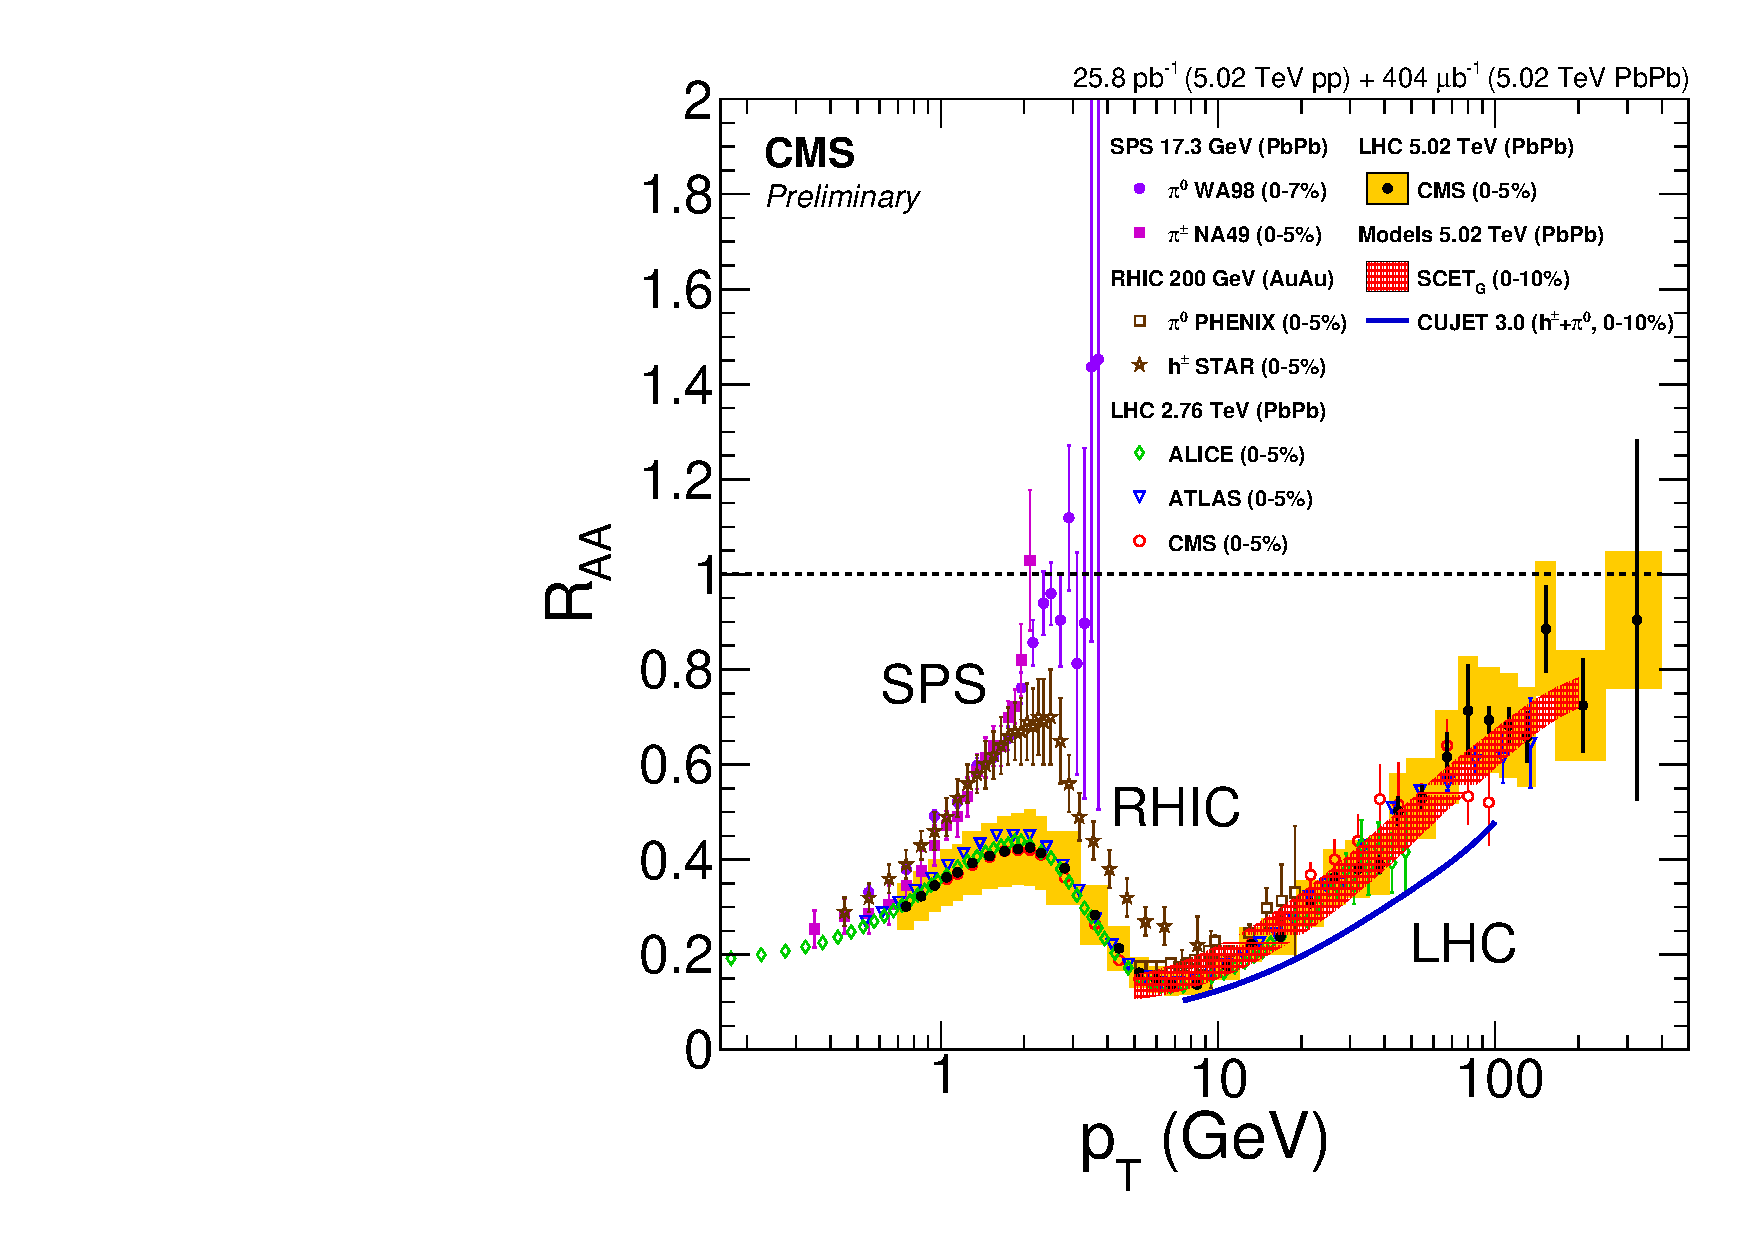
\includegraphics[width=8cm]{FigCap1/CMSRaa.pdf}
  \caption{Measurements of the nuclear modification factors in central heavy-ion collisions at four different center-of-mass energies at SPS~\cite{Aggarwal:2001gn,dEnterria:2004cly,Alt:2007cd}, RHIC~\cite{Adare:2012wg,Adams:2003kv}, and LHC~\cite{Abelev:2012hxa,Aad:2015wga,CMS:2012aa}, compared to predictions of two models from~\cite{Chien:2015vja,Xu:2015bbz}}
  \label{fig:CMSRaa}
\end{figure}
ALICE also measured the nuclear modification factor of identified 
particle species, that can further constrain the models. In Fig.~\ref{fig:PiKPRaa5TeV}
 the $\Raa$ of pions, kaons and protons measured in Pb-Pb collisions 
 at $\sNN = 5.02$ TeV is shown, for different centrality classes. First, it 
 has to be noticed that the suppression has a clear dependence on the 
 collision centrality, since it becomes stronger in more central events, 
 where the medium is more spatially extended, hotter and denser. 
 A second observation from 
  results in Fig.~\ref{fig:PiKPRaa5TeV} is that there is a mass ordering at 
  low $\pt$ that is a direct consequence of the radial flow. In the low-$\pt$
  region, the particle yields in A-A collisions are not governed by the $N_{coll}$ scaling 
  of the yields in pp collisions and the particle spectra are harder in A-A than in pp collisions due to the radial flow. 
  The latter is present at all centralities, but is stronger for central collisions and
  is more pronounced for massive particles.
  
  At high $\pt$
   instead, the suppression is similar for the three species, indicating
    that the medium at high $\pt$ affects the fragmentation of partons in a similar 
    way. Different model calculations were compared to the $\Raa$ 
    measured in different centrality classes by CMS~\cite{CMS:2012aa} 
    and ALICE~\cite{Abelev:2012hxa} and allowed for an extraction of 
    the transport coefficient~\cite{Baier:1996sk} $\hat{q} \approx 1.7-1.9$ 
    GeV$^2/c$ illustrated in~\cite{Burke:2013yra,Liu:2015vna}. 
\begin{figure}[!ht]
  \centering
  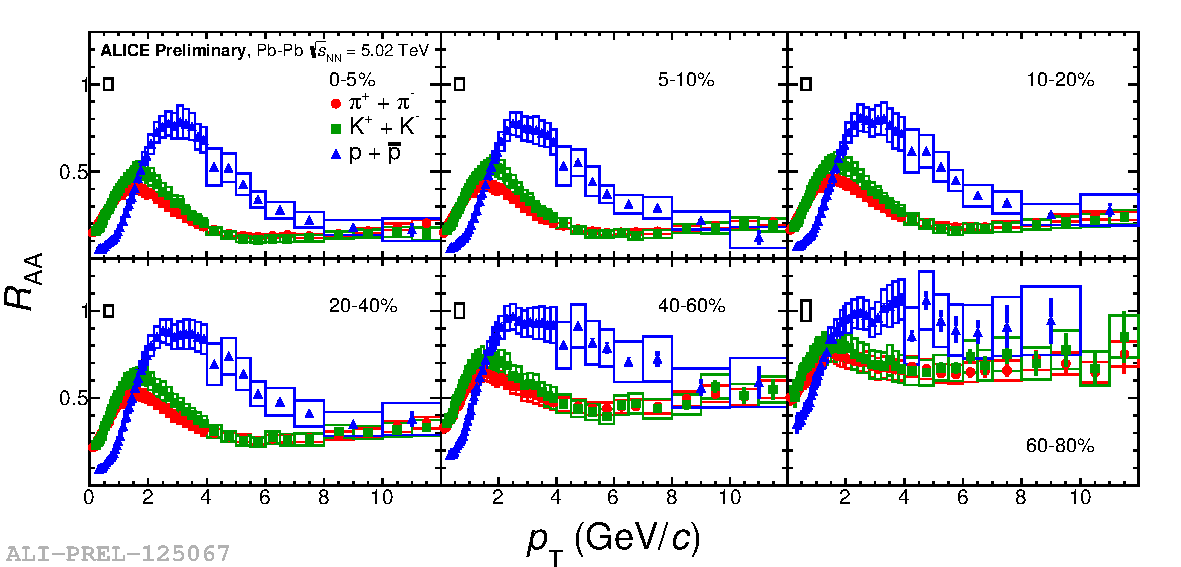
\includegraphics[width=15cm]{FigCap1/KPiPRAA5TeV.pdf}
  \caption{Nuclear modification factor of pions, kaons and protons measured by ALICE in Pb-Pb collisions at $\sNN = 5.02$ TeV in different centrality classes~\cite{Jacazio:2017dvy}.}
  \label{fig:PiKPRaa5TeV}
\end{figure}

\subsubsection{Jets}
The interest in jet measurement with respect to single hadrons is that
the kinematics of the leading parton becomes accessible and we are 
less sensitive to fragmentation effects. Therefore jets are expected to put 
more stringent constraints on assumptions in models for parton energy loss. 
Experimental techniques are now able enough to clearly identify jets 
even in the huge background of high-energy heavy-ion collisions. 
The interaction of the high-$\pt$ partons with the color field of the medium
 induces the radiation of (mostly) soft ($\omega \ll E_{L}$, $E_L$ being the 
 energy of leading parton) and collinear ($k_{\perp} \ll \omega$, $k_{\perp}$ being
 the transverse component of the radiated gluon momentum) gluons. The 
 modeling of a jet emerging from the medium is more complex than that of
  single hadron, since not only the energy loss of the leading parton has to be 
  kept into account, but also the radiated gluons can further re-scatter in the 
  medium inside the jet cone. Thus the total energy inside the jet cone 
  of radius $R$ at the time $t_f$ is:
\begin{equation}
\label{eq:EnergyJet}
E_{jet}(t_f,R) = E_L(t_f) +E_g(t_f,R),
\end{equation}
where $E_g$ is the energy of the radiated gluons, that is defined as:
\begin{equation}
\label{eq:Eg}
E_g(t_f,R) = \int_R d\omega dk^2_\perp \omega f_g(\omega,k^2_\perp,t_f),
\end{equation}
where $f_g(\omega,k_{\perp},t)$ is the double differential distribution of 
the accompanying gluons of the leading parton. It can be obtained after solving 
the following transport equation for the distribution of radiated gluons:
\begin{equation}
\label{eq:RadGluonTransport}
\frac{df_g(w,k_{\perp},t)}{dt} = -\hat{e}\frac{\partial f_g}{\partial \omega} + \frac{1}{4}\hat{q}\nabla^2_{k_{\perp}}f_g + \frac{dN^{rad}_g}{d\omega dk^2_{\perp} dt}.
\end{equation}
The first and the second term in the right-hand side of Eq.~\ref{eq:RadGluonTransport} 
describe the evolution of radiated gluons which can transfer energy 
into the medium via collisional processes (controlled by coefficient 
$\hat{e}$) and accumulate transverse momentum $k_\perp$ 
(coefficient $\hat{q}$). The last term accounts for additional gluon 
radiation coming from emission of the leading parton.\\
\begin{figure}[!ht]
  \centering
  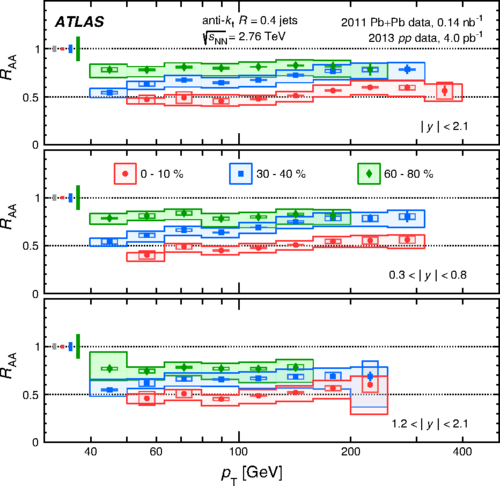
\includegraphics[width=9cm]{FigCap1/ATLASjetsRaa.png}
  \caption{Jet $\RAA$ as a function of $\pt$ in different centrality
intervals in Pb-Pb collisions at $\sNN = 2.76$ TeV~\cite{Aad:2014bxa}. Each panel shows a different range in $|y|$.}
  \label{fig:ATLASjetsRaa}
\end{figure}
\begin{figure}[!ht]
  \centering
  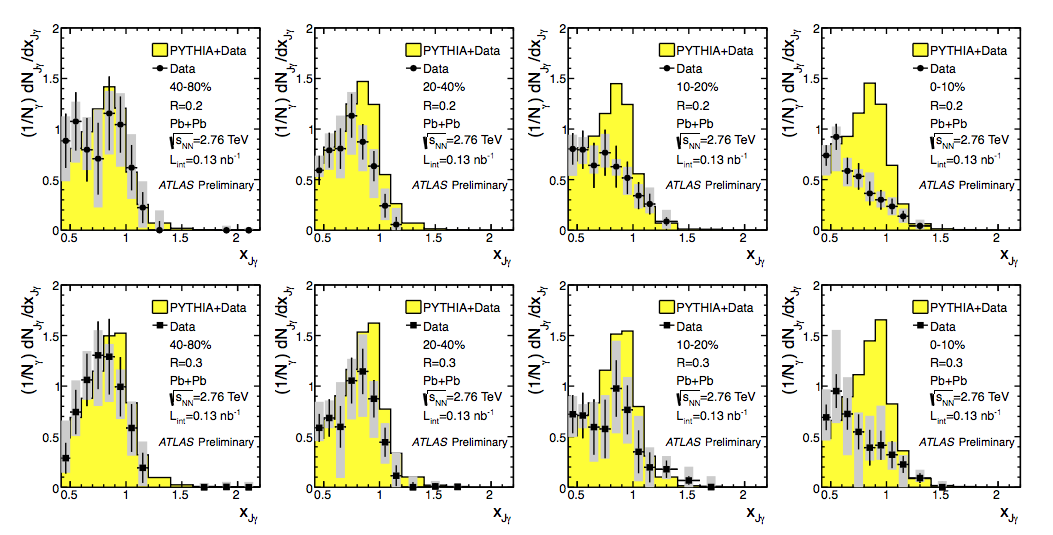
\includegraphics[width=15cm]{FigCap1/ATLASdiijetGammaZ.png}
  \caption{$\frac{1}{N}\frac{dN}{dx_J}$ distribution for reconstructed photon-jet events in Pb-Pb collisions at $\sNN = 2.76$ TeV compared to PYTHIA calculations ($x_J$ is defined in the text)~\cite{ATLAS-CONF-2012-121}. Different centrality classes are shown in each column, while the rows show results for two jet radii, R $= 0.2$ and R $=0.3$.}
  \label{fig:ATLASdijetAsymm}
\end{figure} 
Fig.~\ref{fig:ATLASjetsRaa} shows the jet $\Raa$ measured by ATLAS 
as a function of $\pt$ in different centrality classes and different 
rapidity selections for the three panels~\cite{Aad:2014bxa}. The 
suppression has a clear dependence on the event centrality, while 
is quite flat as a function of $\pt$ in the analysed range from 40 to 400 $\Gevc$. 
This result confirms the strong suppression observed for high-$\pt$ 
charged hadron yield in Pb-Pb relative to pp collisions at LHC energies and reveals that the 
medium is so opaque to quench even the most energetic jets. The 
azimuthal correlations of transverse energy of back-to-back jets 
constitute an other interesting observable to characterize the effect 
of jet-medium interaction. At LHC energies, a large number of dijet 
from back-to-back partons is observed to have an asymmetry in the energy 
of the two reconstructed jets, that can be quantified by 
$x_J = \pt^{jet1}/\pt^{jet2}$. Fig.~\ref{fig:ATLASdijetAsymm} shows the $\frac{1}{N}\frac{dN}{dx_J}$ 
distribution for reconstructed photon-jet events in Pb-Pb collisions at $\sNN = 2.76$ TeV 
compared to PYTHIA calculations~\cite{ATLAS-CONF-2012-121}. 
Each column corresponds to different centrality classes, while the 
rows show results for two jet radii, R $= 0.2$ and R $=0.3$. In more 
peripheral collisions the $x_J$ distribution is peaked towards 1, thus 
meaning that higher $\pt$ dijets tend to be balanced in momentum. 
Moving towards more central events, the $x_J$ distribution appears 
flatter around $0.5 < x_J<1$, to eventually become peaked around 
$x_J \sim 0.5$ in the 10\% more central events.
This is understood in terms of different path 
lengths that the two partons have to traverse in the medium. In general, 
measurements of inclusive jets and dijet suffer from the fact that leading jets 
experience themselves some energy loss, thus the energy of the jet is not 
fully defined. Using weak bosons (Z or W) or photons, that do not interact 
with the medium, to replace one of the two jets allows us to fully calibrate the 
initial energy of the jet, as explained in~\cite{Wang:1996yh}. 

% \begin{figure}[!ht]
%   \centering
%   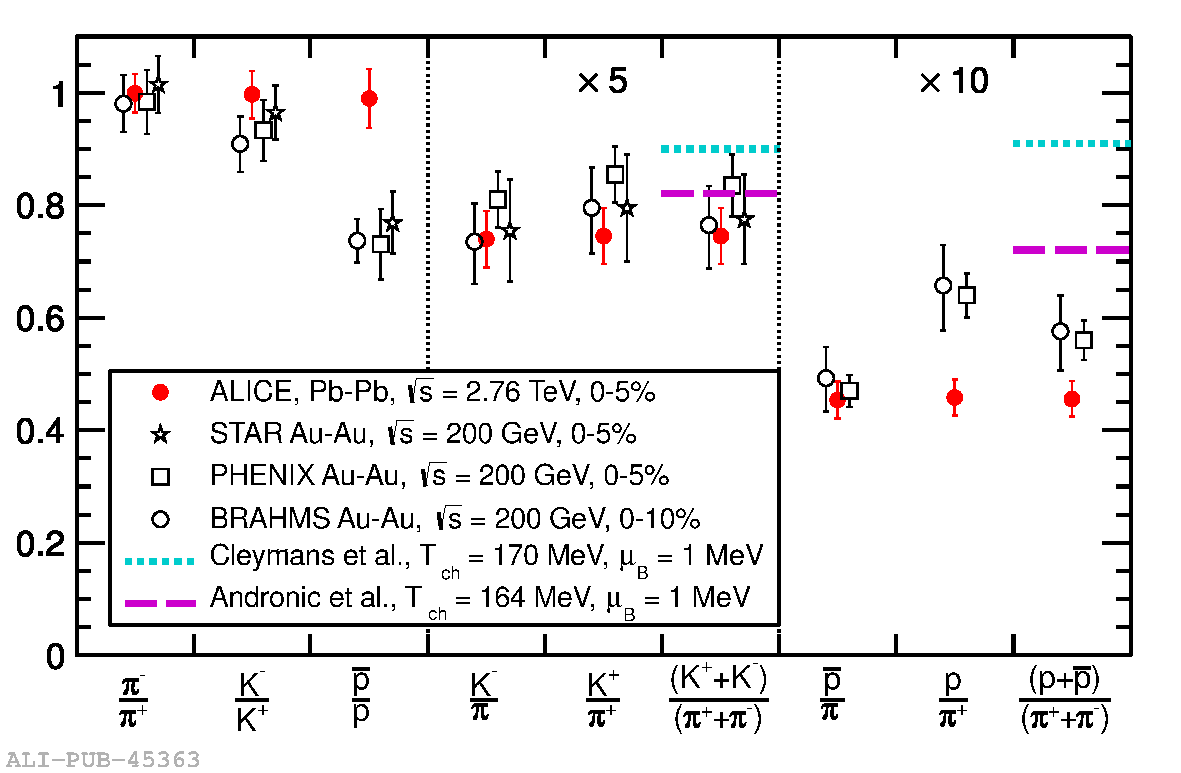
\includegraphics[width=10cm]{FigCap1/CentralPbPbRatiosThermalModels.pdf}
%   \caption{Mid-rapidity particle ratios, compared to RHIC results~\cite{Abelev:2008ab,Adler:2003cb,Arsene:2005mr} and predictions from thermal models~\cite{Andronic:2008gu,Cleymans:2006xj} for central Pb-Pb collisions at the LHC (combined statistical and systematic errors)~\cite{Abelev:2012wca}. }
%   \label{fig:CentralPbPbRatiosThermalModels}
% \end{figure}
\subsection{Quarkonium production}
\label{sec:Quarkonium}
Quarkonium, the bound state of a $c\bar{c}$ (charmonium) or $b\bar{b}$ 
(bottomonium) pair, was proposed from the very beginning as one of the 
most powerful signatures of the QGP formation.
The signature given by the J/$\psi$ vector meson yield is of particular interest
in the view of assessing about the formation of a deconfined medium.
The J/$\psi$ mesons, and more in general the charmonium states, are formed 
by a $c\bar{c}$ quark pair, that can only be produced (due to the large mass) 
in the initial hard parton scatterings, occurring before the formation of the 
Quark-Gluon Plasma. Theoretical calculations based on lattice QCD 
predict a J/$\psi$ suppression to be induced by the screening of the color 
force in a deconfined medium, due to the presence of free 
color charges, which becomes stronger as the temperature 
increases~\cite{Abreu:2000ni,Matsui:1986dk}. 
J/$\psi$ suppression was first observed at the SPS in Pb-Pb collisions, by 
the NA38 and NA50 experiments~\cite{Abreu:2000ni}.
The ratios between the observed J/$\psi$ yield and the expected one 
based on the so-called ``ordinary nuclear absorption" measured in p-A 
collisions are shown in Fig.~\ref{fig:JPsiSuppressionNA50} 
as a function of the energy density $\epsilon$ of the medium traversed by the charmonium state. 
The results showed that for energy densities up to $\epsilon \lesssim 2.5$ GeV/fm$^3$, 
the yield of the J/$\psi$ meson is compatible with measurements in pp 
and p-A collisions, in which only ordinary nuclear absorption is present. In Pb-Pb 
collisions, instead, where $\epsilon$ becomes larger, there is a clear deviation from 
unity of the ratio measured/expected, which was interpreted as a first indication of 
charmonium suppression due to colour screening in the QGP.
\begin{figure}[!ht]
  \centering
  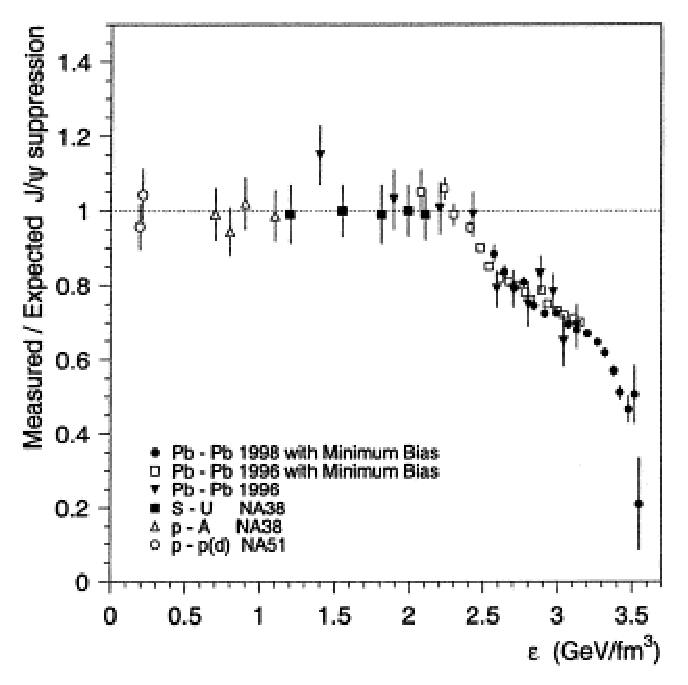
\includegraphics[width=6.6cm]{FigCap1/JPsiSuppressionNA50.eps}
  \caption{Ratio between measured J/$\psi$ production and expected one in pp, p-A and A-A collisions as function of the energy density of the medium ~\cite{Abreu:2000ni}.}
  \label{fig:JPsiSuppressionNA50}
\end{figure}
Clear signs of J$/\psi$ suppression were indeed measured at the SPS, as a 
consequence of the strong color field of the plasma~\cite{Abreu:2000ni}. 
Charmonium states were also expected to melt at different temperatures of 
the plasma, accordingly to their binding energy, giving rise to a sequential melting 
scenario~\cite{Du:2015wha,Digal:2001ue}. What turned 
out to be unexpected when data at higher collision energies became available 
was that the RICH~\cite{Adare:2011yf,Adare:2006ns} J$/\psi$ suppression 
had the same magnitude as the one observed at the SPS~\cite{Scomparin:2007rt}.
At LHC energies, a reduced suppression as compared to lower
collision energies was observed~\cite{Abelev:2013ila}.
In Fig.~\ref{fig:RaaJPsi} the ALICE measurements 
of J$/\psi$ $\Raa$ in Pb-Pb collisions at $\sNN = 2.76$ TeV~\cite{Abelev:2013ila} 
and at $\sNN = 5.02$ TeV~\cite{Adam:2016rdg} are compared to measurements at 
RHIC~\cite{Adare:2011yf} for Au-Au collisions at $\sNN = 200$ GeV. In the left panel of Fig.~\ref{fig:RaaJPsi} 
the $\Raa$ is presented as a function of the centrality and shows smaller J$/\psi$ suppression 
at the higher energies, where the measurement is for J$/\psi$ with $\pt < 8 \Gevc$. 
The centrality dependence is similar at the two LHC energies. 
In the right panel of the same figure, the 
dependence on $\pt$ reveals that the different suppression at different $\sNN$ is mostly
in the low-$\pt$ region.
CMS measured the J$/\psi$ $\Raa$ 
in the high $\pt$ region, up to $\pt = $ 30 $\Gevc$, confirming a stronger suppression
($\RAA \approx 0.3$ for most central events) with respect to 
low $\pt$~\cite{Khachatryan:2016ypw}. All these observations can be 
explained by a (re)generation effect of uncorrelated $c$ and $\bar{c}$ quarks, relevant at LHC energies due to the 
large production cross-section of $c\bar{c}$ quark pairs. 
An other observable that is sensitive to the J$/\psi$ production 
mechanism is the elliptic flow $v_2$. If the J$/\psi$ is produced by coalescence 
of charm quarks, and the charm thermalises in the medium, the J$/\psi$ 
should inherit the flow of the quarks and show a positive $v_2$. 
A non-zero $v_2$ could also be observed due to the path-length dependence of charmonium
in-medium energy loss, thus the final $v_2$ may be an 
interplay of multiple effects. Fig.~\ref{fig:JPsi} presents recent measurements 
by ALICE of J$/\psi$ $v_2$ at forward and mid-rapidity in Pb-Pb collisions at 
$\sNN = 5.02$ TeV for semi-central events (20-40\% centrality class)~\cite{Acharya:2017tgv}, 
compared with some of the available theoretical models. At forward rapidity, 
the maximum $v_2$ is reached in $4 < \pt < 6\; \Gevc$, with a 
significance for non-zero $v_2$ larger than $6.6\sigma$. Model calculations 
that include (re)combination of thermalised charm and beauty quarks as 
source of J$/\psi$ production, together with a path-length dependent in-medium 
energy loss can describe the data at low $\pt$, but fail in 
reproducing the measured shape at higher $\pt$, suggesting a missing mechanism in the 
model ({\it Du et al.} in Fig.~\ref{fig:JPsi}~\cite{Du:2015wha}). The model by 
{\it Zhou et al.}~\cite{Zhou:2014kka} includes, in addition to the cited components, 
a contribution from the modification of quarkonium production in the presence 
of a strong magnetic field in the early stage of the heavy-ion collision~\cite{Guo:2015nsa}. 
The $v_2$ resulting from the different in-plane and out-of-plane survival 
probabilities of primordial J$/\psi$ is shown as dashed red and dash-dotted 
orange lines. At LHC energies also the bottomonium states have been 
measured, opening the way to precision studies for the $\Upsilon$({\it n}S) 
family. Due to smaller production cross-section of $b$ quarks compared to $c$ quarks, 
effects of coalescence are
expected to be of smaller impact with respect to charmonium~\cite{Andronic:2015wma}. 
A sequential suppression pattern is expected also for $b\bar{b}$ states, due to 
different binding energies of the bottomonium states. CMS measured 
the $\Raa$ of $\Upsilon$(1S), $\Upsilon$(2S) and $\Upsilon$(3S) as a 
function of the centrality in Pb-Pb collisions at 
$\sNN = 2.76$ TeV~\cite{Khachatryan:2016xxp} (Fig.~\ref{fig:JPsi}, right) and at 
$\sNN = 5.02$ TeV~	\cite{Sirunyan:2017lzi}. The $\RAA$ in the right panel of Fig.~\ref{fig:JPsi} shows a 
suppression for the $\Upsilon$(2S) state (factor of 8), that is larger with 
respect to the $\Upsilon$(1S) state (factor of $\sim$ 2), while for 
the $\Upsilon$(3S) only an upper limit could be determined.
The measured suppression of the three $\Upsilon$ states is compatible 
with theoretical models of a sequential melting of quarkonium states in a 
hot medium~\cite{Khachatryan:2016xxp}.
%~\cite{Sirunyan:2016znt}
\begin{figure}[!ht]
  \centering
  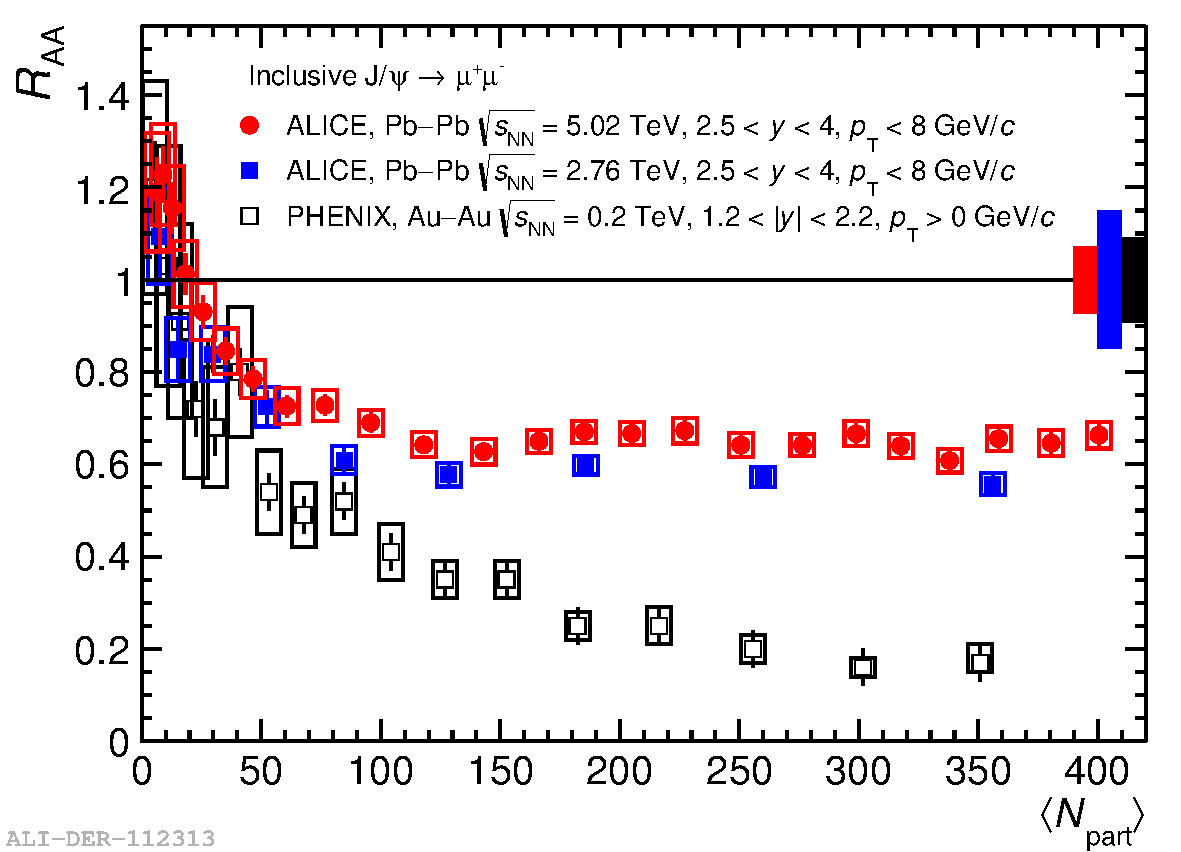
\includegraphics[width=7cm]{FigCap1/RaaJPsiAlicePhenix.pdf}
  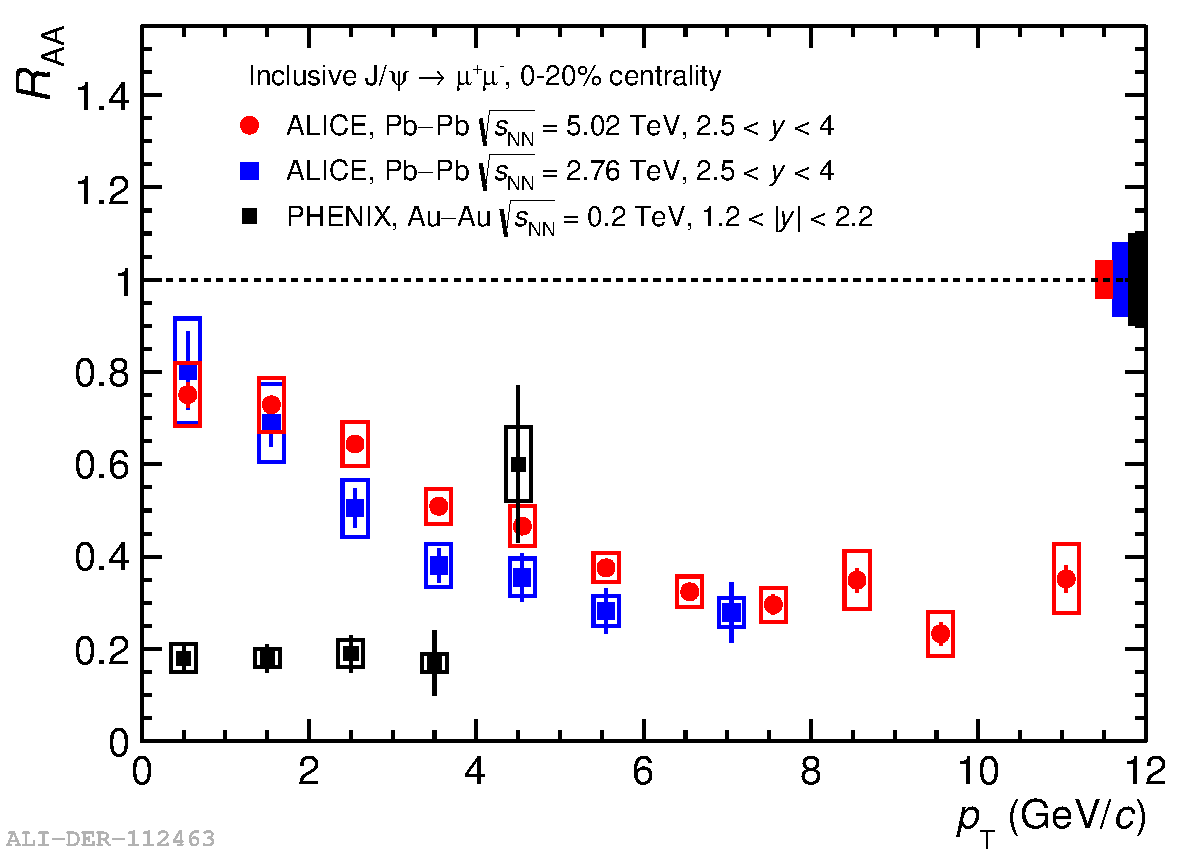
\includegraphics[width=7cm]{FigCap1/RaaJPsiAlicePhenixVsPt.pdf}
  \caption{Centrality (left) and transverse momentum (right) dependence of the J$/\psi$ $\RAA$ measured by ALICE in Pb-Pb collisions at $\sNN = 2.76$ TeV~\cite{Abelev:2013ila} (blue) and at $\sNN = 5.02$ TeV~\cite{Adam:2016rdg} (red) compared to PHENIX~\cite{Adare:2011yf} results Au-Au collisions at $\sNN = 200$ GeV.}
  \label{fig:RaaJPsi}
\end{figure}

\begin{figure}[!ht]
  \centering
  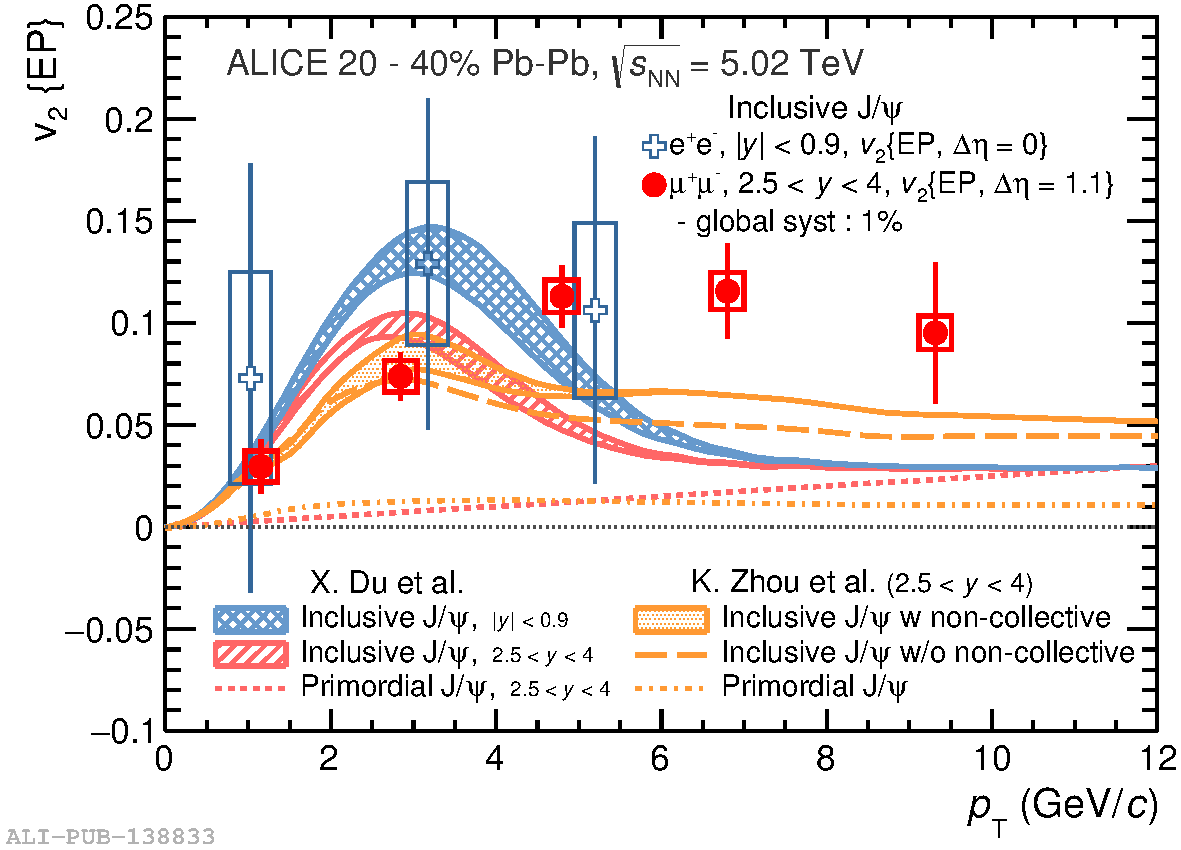
\includegraphics[width=7cm]{FigCap1/JPsiV2Models.pdf}
  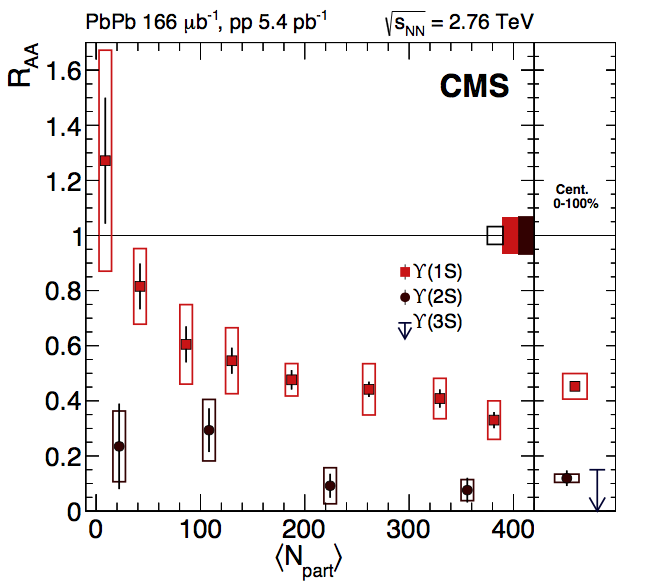
\includegraphics[width=6cm]{FigCap1/RaaUpsilonCMS.png}
  \caption{Left: inclusive J$/\psi$ $v_2(\pt)$ at forward and mid-rapidity for semi-central (20-40\%) Pb-Pb collisions at $\sNN =$ 5.02 TeV~\cite{Acharya:2017tgv}. Calculations from transports model from Refs.~\cite{Du:2015wha} and~\cite{Zhou:2014kka} are also shown. Right: nuclear modification factors of $\Upsilon$(1S) and $\Upsilon$(2S) meson production in Pb-Pb collisions measured by CMS, as a function of centrality.
The upper limit derived on the nuclear modification factor for $\Upsilon$(3S) is represented with an arrow in the centrality integrated panel on the right~\cite{Khachatryan:2016xxp}. }
  \label{fig:JPsi}
\end{figure}

\subsection{Latest discoveries in small systems}
In 2010 CMS discovered first signals of long-range rapidity correlations in 
high-multiplicity pp collisions at $\sqrt{s} = $ 7 TeV~\cite{Khachatryan:2010gv}, an effect that 
resulted quite unexpected to be found in small systems. Such correlations
were already observed in Au-Au collisions at RICH~\cite{Alver:2008aa,Alver:2009id,Abelev:2009jv}
and naturally explained in terms of collective expansion of the medium formed in the collisions.
This observation paved the way to search further signals of collective 
behaviours in small systems. 
The interest in the angular correlations among particles lays in the possibility 
to reveal the underlying mechanisms of particle production. In~\cite{Khachatryan:2010gv}, 
CMS studied the two-dimensional $\Delta \eta$-$\Delta \phi$ correlation 
function, where $\Delta \eta$ is the difference in pseudo-rapidity between 
two particles and $\Delta \phi$ is the difference in their azimuthal angle $\phi$. The $\pt$-inclusive two-particle 
correlation, as a function of $\Delta \eta$ and $\Delta \phi$ is defined as:
\begin{equation}
\label{CorrelationFnc}
R(\Delta \eta,\Delta \phi) = \Big \langle (\langle N \rangle -1) \Big (\frac{S_N(\Delta \eta,\Delta \phi)}{B_N(\Delta \eta,\Delta \phi)} -1\Big )\Big \rangle,
\end{equation}
where (i) $S_N(\Delta \eta,\Delta \phi)$ is the correlation function for the signal distribution,
determined by counting all particle pairs in each event within a multiplicity bin, 
(ii) $B_N(\Delta \eta,\Delta \phi)$ is the correlation function for the background distribution, determined
  by correlating each charged particle of one event with every particle from 
a different event within the same multiplicity bin, (iii) the average is made over all the multiplicity bins of the analysis.
\iffalse
We can define now two correlation functions, the first one, $S_N(\Delta \eta,\Delta \phi)$ for the signal distribution:
\begin{equation}
\label{SignalDistribution}
S_N(\Delta \eta,\Delta \phi) = \frac{1}{N(N-1)}\frac{d^2N^{signal}}{d\Delta \eta d\Delta \phi}
\end{equation}
and the second, $B_N(\Delta \eta,\Delta \phi)$, for the background distribution:
\begin{equation}
\label{BkgDistribution}
B_N(\Delta \eta,\Delta \phi) = \frac{1}{N^2}\frac{d^2N^{mixed}}{d\Delta \eta d\Delta \phi}.
\end{equation}
$S_N(\Delta \eta,\Delta \phi)$ can be determined by counting all particle pairs in each 
event within a multiplicity bin, using the weighting factor $N(N-1)$. $B_N(\Delta \eta,\Delta \phi)$ 
is obtained instead by correlating each charged particle of one event with every particle from 
a different event within the same multiplicity bin. Finally, the $\pt$-inclusive two-particle 
correlation, as a function of $\Delta \eta$ and $\Delta \phi$ is obtained as:
\begin{equation}
\label{CorrelationFnc}
R(\Delta \eta,\Delta \phi) = \Big \langle (\langle N \rangle -1) \Big (\frac{S_N(\Delta \eta,\Delta \phi)}{B_N(\Delta \eta,\Delta \phi)} -1\Big )\Big \rangle,
\end{equation}
where the average is made over all the multiplicity bins of the analysis. 
\fi
By using the ratio of $S_N(\Delta \eta,\Delta \phi)$ and $B_N(\Delta \eta,\Delta \phi)$, 
detector effects such as tracking inefficiencies, non-uniform acceptances, etc, are 
automatically corrected. In Fig.~\ref{fig:CMSLongRangeRidge_pp7TeV}, $R(\Delta \eta,\Delta \phi)$ 
is plotted for high-multiplicity events ($N_{tracks} > 110$) in pp collisions at $\sqrt{s} = $ 7 TeV, 
selecting tracks with $1 <\pt < 3\; \Gevc$. Several correlation structures are present. 
The narrow peak at $(\Delta \eta, \Delta \phi) \approx (0,0)$ is the contribution 
from jet-like particle production (near-side peak). The broad ridge around $\Delta \phi \approx \pi$ 
is due to the fragmentation of back-to-back jets (away-side ridge). The ridge-like 
structure that appears around $\Delta \phi \approx 0$ was unexpected,
 indeed never observed in two-particle correlations in pp data, neither in minimum-bias 
 events nor in high-multiplicity low $\pt$ events. Event generators, such as PYTHIA, did not reproduce the 
 observed structure, that seems to resemble hydrodynamic behaviors of heavy-ion 
 collisions~\cite{Alver:2008aa,Alver:2009id,Abelev:2009jv}, and the physical origin is still not clear.
\begin{figure}[!ht]
  \centering
  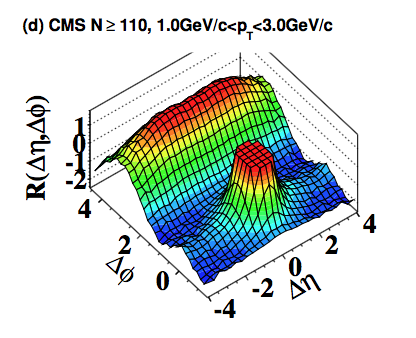
\includegraphics[width=7cm]{FigCap1/CMSLongRangeRidge_pp7TeV.png}
  \caption{Two-particle correlation functions in $\eta$-$\phi$ for 7 TeV pp collisions, in high multiplicity events ($N_{trk}>110$), with 1 $< \pt < 3 \Gevc$~\cite{Khachatryan:2010gv}.}
  \label{fig:CMSLongRangeRidge_pp7TeV}
\end{figure}
From this first observation, many studies have been done to unravel the nature of the 
long-range near side peak. Correlations among several produced particles have been explored, 
since this allows to further suppress short-range particle correlations, 
such as jets or resonance decays, in order to further investigate the collective nature 
of the observed azimuthal correlations. One of the most used methods is the 
Q-cumulants method. Following the approach in~\cite{Bilandzic:2010jr}, the 
correlations of two, four and six particles are evaluated as:
\begin{equation}
\label{correlations}
\begin{aligned}
\langle \langle 2 \rangle \rangle &= \langle \langle e^{in(\phi_1 -\phi_2)} \rangle \rangle &\\
\langle \langle 4 \rangle \rangle &= \langle \langle e^{in(\phi_1 + \phi_2 -\phi_3 - \phi_4)} \rangle \rangle &\\
\langle \langle 6 \rangle \rangle &= \langle \langle e^{in(\phi_1 + \phi_2 +\phi_3 - \phi_4- \phi_5- \phi_6))} \rangle \rangle,&
\end{aligned}
\end{equation}
where $\phi_i$ are the azimuthal angles of the correlated particles in an event, $n$ is the harmonic number and $\langle \langle ... \rangle \rangle$ indicates the average over all combinations from all events in a given multiplicity range. The cumulants are obtained as follows:
\begin{equation}
\label{eq:cumulants}
\begin{aligned}
\begin{split}
c_n\{4\} &= \langle \langle 4 \rangle \rangle - 2 \times  \langle \langle 2 \rangle \rangle^2 \\
c_n\{6\} &= \langle \langle 6 \rangle \rangle - 9 \times  \langle \langle 4 \rangle \rangle \langle \langle 2 \rangle \rangle + 12 \times \langle \langle 2 \rangle \rangle^3.
\end{split}
\end{aligned}
\end{equation}
Finally the Fourier harmonics $v_n$ coefficients are obtained from cumulants in Eq.~\ref{eq:cumulants} as:
\begin{equation}
\begin{aligned}
v_n \{4\} = \sqrt[4]{-c_n\{4\}} \\
v_n \{6\} = \sqrt[6]{\frac{1}{4}c_n\{6\}}.
\end{aligned}
\end{equation}
\begin{figure}[!ht]
  \centering
  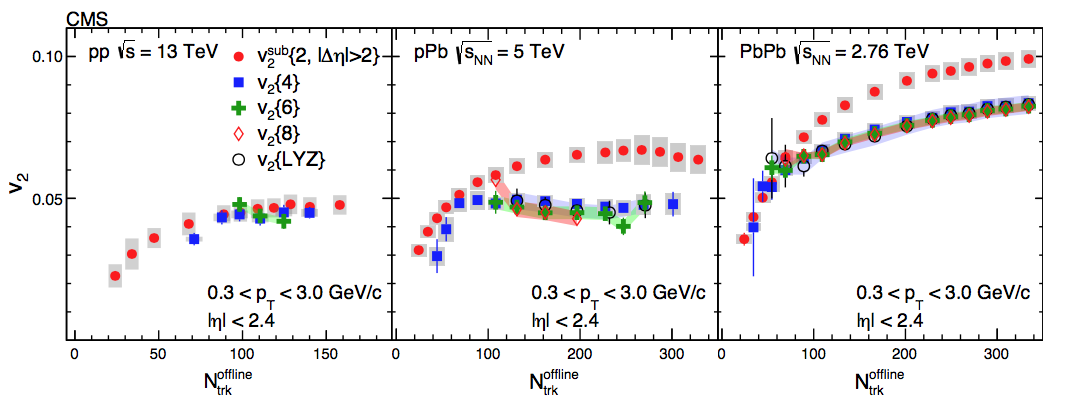
\includegraphics[width=15cm]{FigCap1/v2CumulantsCMS.png}
  \caption{$v_2^{sub} \{2\, |\Delta \eta| > 2\}$, $v_2 \{4\}$, $v_2 \{6\}$, $v_2 \{8\}$ 
  and $v_2 \{LYZ\}$ as a function of the multiplicity, 
  in the interval $0.3 < \pt < 3 \Gevc$ and $|\eta| < 2.4$~\cite{Khachatryan:2016txc} measured by CMS, in pp, p-Pb and Pb-Pb collisions.}
  \label{fig:CumulantsCMS}
\end{figure}
In the left panel of Fig.~\ref{fig:CumulantsCMS}, the $v_2 \{4\}$, $v_2 \{6\}$
measured by CMS in pp collisions at $\sqrt{s} = 13$ TeV are shown as a 
function of the particle multiplicity, in the interval $0.3 < \pt < 3 \; \Gevc$ and 
$|\eta| < 2.4$. In the middle and right panels of the same figure, also the $v_2 \{8\}$ and $v_2 \{ {\rm LYZ} \}$ 
(from Lee-Yang zeros method~\cite{Bhalerao:2003yq}) coefficients are shown, for p-Pb and Pb-Pb collisions
at $\sNN = $ 5 TeV and $\sNN = $ 2.76 TeV respectively.
$v_2 \{8\}$ and $v_2 \{ {\rm LYZ} \}$ are less affected by non-flow correlations, 
thus are expected to give the 
cleanest values of the genuine collective flow.
The values of $v_2 \{4\}$, $v_2 \{6\}$ and of $v_2 \{8\}$ and  $v_2 \{ {\rm LYZ} \}$, where present, are compatible among 
them in each of the three colliding system. This supports the idea 
of a collective behaviour behind the long-range correlations observed in pp 
collisions. In alternative to the classical scenario of position-space
anisotropy that must be transposed into final observed momentum-space anisotropies, other theoretical 
calculations, such as the color glass condensate glasma model~\cite{Schenke:2016ksl}, 
interpret the collective behaviour as due to momentum space-anisotropies that are
already present before the collision via initial interactions of gluons inside the projectile proton or
nucleus. Besides, in Fig.~\ref{fig:CumulantsCMS} the 
$v_2^{sub} \{2$, $|\Delta \eta| > 2\}$, defined from two-particle 
$\Delta \eta$, $\Delta \phi$ correlation after subtraction of jet correlations from low-multiplicity events, 
is also shown. Some hydrodynamical models interpret the similar magnitude 
of $v_2 \{4\}$ and $v_2^{sub} \{2$, $|\Delta \eta| > 2\}$ in pp collisions as the 
consequence of smaller number of initial fluctuating source than in p-Pb and 
Pb-Pb collisions.\\
Recently, ALICE reported about the first observation of strangeness production
 enhancement in high-multiplicity pp collisions~\cite{ALICE:2017jyt}. As 
 anticipated in~\ref{subsec:StrangEnhancSPS}, strangeness enhancement 
 was originally proposed as a signature of the Quark-Gluon Plasma and 
 verified to be even more pronounced for multi-strange baryons. The production 
 of strange hadrons in heavy-ion collisions can be described using a 
 grand-canonical statistical model and does not show a significant dependence 
 on the collision centrality, if one excludes the very peripheral events. For the latter,
  the relative yield of strange particles to pions becomes very similar to what 
  observed in pp and in p-Pb~\cite{Abelev:2013haa,Adam:2015vsf} collisions, and this is understood
  in terms of canonical suppression~\cite{Tounsi:2001ck}. In~\cite{ALICE:2017jyt}, ALICE presented the
   measurement of the production of primary strange ($K^0_S,\; \Lambda,\; \bar{\Lambda}$) 
   and multi-strange ($\Xi^-,\; \Xi^+,\; \Omega^-,\; \Omega^+$) hadrons in pp 
   collisions at $\sqrt{s} = 7$ TeV. Fig.~\ref{fig:StrangenessALICEpp} (left panel) 
   shows the $\pt$-differential yields of 
   $K^0_S,\; \Lambda + \bar{\Lambda},\; \Xi^- + \Xi^+,\; \Omega^- + \Omega^+$ 
   at mid-rapidity, for a selection of classes of events with progressively lower 
   multiplicity, indicated by roman numbers in bracket in the figure. It can be 
   noticed that the $\pt$ spectra become harder as the multiplicity increases, 
   and the hardening becomes stronger with increasing particle mass. This is
    a feature already observed in p-Pb collisions~\cite{Abelev:2013haa} and 
    typically characterizing Pb-Pb collisions, where they are described in terms 
    of relativistic hydrodynamical expansion. A simultaneous fit with the 
    blast-wave model to all $\pt$ spectra in the common highest multiplicity class 
    (I in Fig.~\ref{fig:StrangenessALICEpp} left) and in defined $\pt$ ranges allowed the 
    extraction of the chemical freeze-out temperature $T_{fo} = 163 \pm 10$ 
    MeV and the transverse velocity of the bulk 
    $\langle \beta_{\perp} \rangle = 0.49 \pm 0.02$. The $\pt$ distribution were
     then fitted in their full $\pt$ range using a Tsallis-Lèvy function to obtain the 
     $\pt$-integrated yields. Finally, the right panel of Fig.~\ref{fig:StrangenessALICEpp}
      shows the ratio of $\pt$-integrated hadron yields to the pion yields, as a 
      function of the charged-particle multiplicity, together with the measurements
       in p-Pb ($\sNN = 5.02$ TeV) and Pb-Pb ($\sNN = 2.76$ TeV) collisions. 
       Despite the different energy of the collisions, the ratios show a smooth 
       increase from pp to most central Pb-Pb collisions, with the highest multiplicity 
       points in pp being fully compatible with the magnitude of the enhancement in 
       p-Pb at same multiplicity values or in most peripheral Pb-Pb collisions. At higher multiplicities,
       the ratios in Pb-Pb collisions do not show particular dependence on the collision centrality. This 
       suggests that the mechanism of strangeness enhancement is rather related
        with the characteristics of the final state produced in the collisions, than the
         characteristics of the collision itself. Still, the physical mechanism remains 
         unclear, since the available models fail in reproducing at the same time both
          the ratios in Fig.~\ref{fig:StrangenessALICEpp} and the $\pt$-integrated 
          proton to pion ratios at mid-rapidity~\cite{ALICE:2017jyt}.
\begin{figure}[!ht]
  \centering
  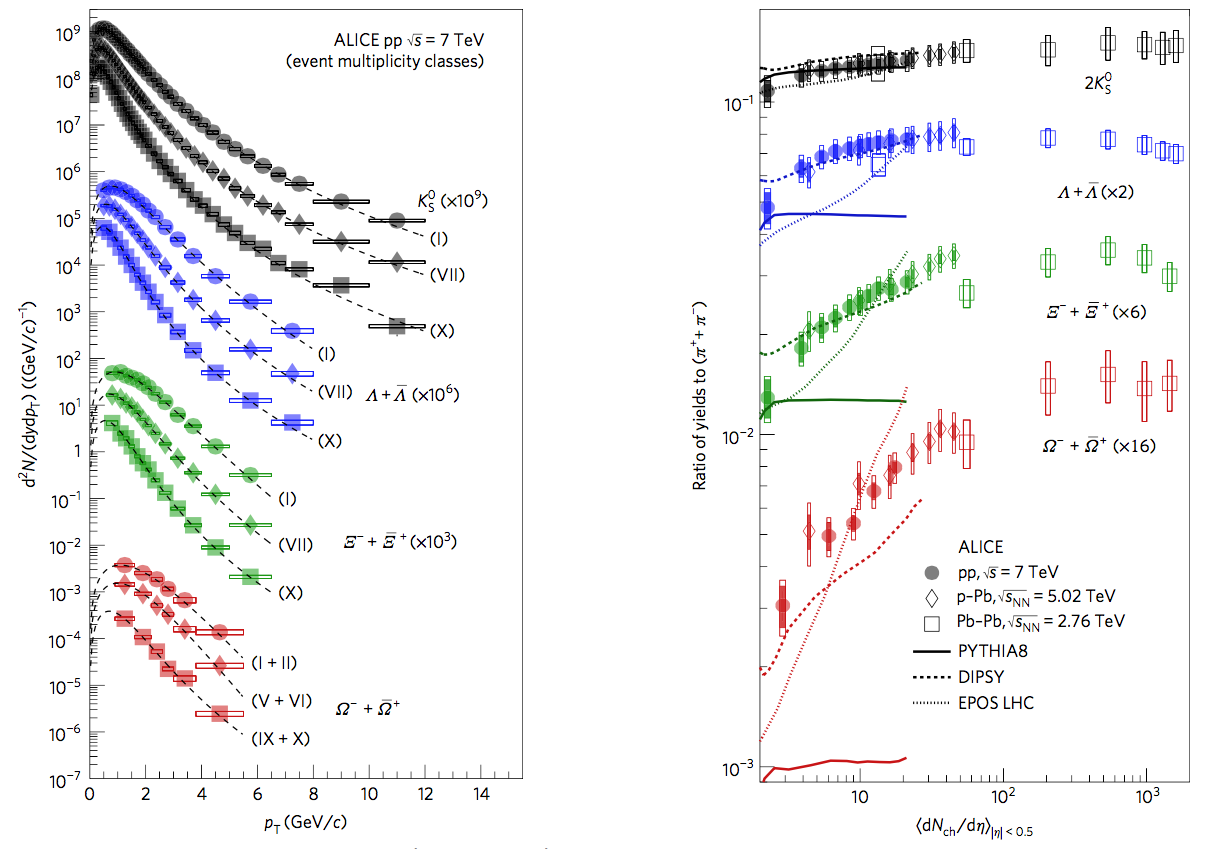
\includegraphics[width=14cm]{FigCap1/StrangenessALICEpp.png}
  \caption{Left: $\pt$-differential yields of $K^0_S,\; \Lambda + \bar{\Lambda}, \Xi^- + \Xi^+,\; \Omega^- + \Omega^+$ at mid-rapidity, for a selection of classes of events with progressively lower multiplicity. The Tsallis-Lèvy fit is shown as dashed line. Right: $\pt$-integrated ratios of $K^0_S,\; \Lambda + \bar{\Lambda},\; \Xi^- + \Xi^+,\; \Omega^- + \Omega^+$ to pion yield ($\pi^- + \pi^+$) as a function of $\langle dN_{ch}/d\eta \rangle$ at mid-rapidity~\cite{ALICE:2017jyt}.}
  \label{fig:StrangenessALICEpp}
\end{figure}














\chapter{Heavy flavours} % Main chapter title
\label{Chapter2} % For referencing the chapter elsewhere, use \ref{Chapter1} 

\section{The importance of being heavy}
\label{sec:introChap2}
Hadrons carrying heavy flavour (charm or beauty quarks) 
constitute a powerful probe to study 
the properties of the Quark-Gluon Plasma created in high-energy 
heavy-ion collisions. Heavy quarks are produced in initial hard parton-scattering processes
of the nucleon-nucleon collisions and on short time scales compared 
to the QGP formation time~\cite{Liu:2012ax},
$\tau_0 \sim 1/Q \sim 0.1-1$ fm/c, where $Q$ is the virtuality of the process. 
The minimum virtuality in the production of $c\overline{c}, b\overline{b}$ pair 
corresponds indeed to $2\, m_{c,b}$
implying a space-time scale of $\sim 0.07$ fm for charm and 
$\sim 0.02$ fm for beauty. Furthermore, in contrast with light quarks and gluons, that can be produced or annihilated 
during QGP evolution, heavy quarks have negligible annihilation 
rate~\cite{BraunMunzinger:2007tn} and secondary "thermal" 
charm production from processes like $gg \rightarrow c\overline{c}$ is 
expected to be negligible in the QGP~\cite{Zhang:2007dm}, 
unless the iniial QGP temperatures occur to be much larger than 
those currently reachable at colliders. Therefore,
heavy quarks preserve their identity when traversing 
the fireball and can be used as a probe
to study the interaction with the medium
 constituents, in particular getting access to the 
transport coefficients of the QGP.\\
There are different ways to experimentally detect hadrons 
containing heavy flavours:
\begin{itemize}
\item full reconstruction of exclusive decay channels, 
like $\DtoKpi$ or $B^0 \rightarrow J/\psi K^0_S$;
\item detection of leptons from heavy-flavour hadron decays, for example 
$D, B \rightarrow e, \mu + X$;
\item selection of semi-inclusive decays, 
for example $J/\psi$ mesons displaced 
from the primary vertex (thus, coming from beauty decay) or $\Lambda_c$ and
$\Xi_c$ reconstruction from $e\, \Lambda$ and $e\, \Xi$ pairs;
\item reconstruction of $c-$ and $b-$jets.
\end{itemize}
\section{Heavy-quark production in pp collisions}
\label{sec:HFpp}
The study of heavy flavours in pp collisions is an 
important benchmark of perturbative QCD calculations. 
The large mass of these quarks acts as a cut off; it prevents 
indeed from divergencies in calculation that arise
from collinear gluon radiation and that are suppressed 
in case of massive quarks due to the
so-called dead-cone effect~\cite{Dokshitzer:1991fd}. 
For this reason, perturbative calculations are applicable down to low $\pt$ 
as well as the computation of the total cross-section. 
The two processes responsible for heavy-quark production 
at the leading order in perturbative theory are 
$q \overline{q} \rightarrow Q \overline{Q}$ and $gg \rightarrow Q \overline{Q}$, 
whose corresponding diagrams are
shown in Fig.~\ref{fig:LOdiagrams}. The relative production 
rates for heavy quarks of mass 
$m_1$ and $m_2$ behave, at high energy, as~\cite{Mangano:1997ri}:
\begin{equation}
\begin{aligned}
\frac{\sigma (gg \rightarrow Q_1 \overline{Q}_1)}{\sigma (gg \rightarrow Q_2 \overline{Q}_2)} & \rightarrow 1 - \frac{{\rm log}(m_1^2/m_2^2)}{{\rm log}(s/m_2^2)}, \\
\frac{\sigma (q \overline{q} \rightarrow Q_1 \overline{Q}_1)}{\sigma (q \overline{q} \rightarrow Q_2 \overline{Q}_2)} & \rightarrow 1 - \mathcal{O} (m_1^4/s^2),
\end{aligned}
\end{equation}
hence, at large center-of-mass energy $s$, the 
$q \overline{q} \rightarrow Q \overline{Q}$ process
vanishes more quickly. In the left panel of Fig.~\ref{fig:HQxsecPPcoll}
 the inclusive production cross-section in pp collisions,
as a function of center-of-mass energy, for charm, bottom, 
top quark pairs is shown~\cite{Mangano:1997ri}.
\begin{figure}[!ht]
  \centering
  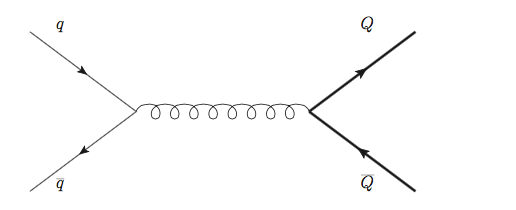
\includegraphics[width=8cm]{FigCap2/Feymann1.png}
  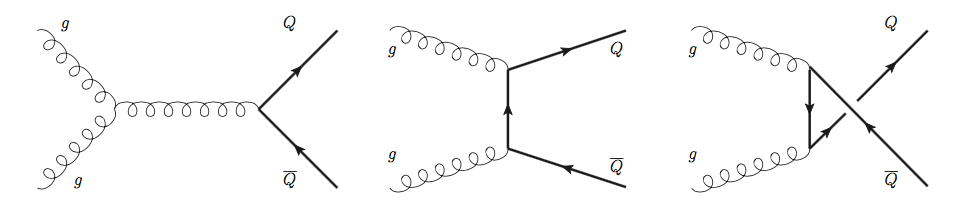
\includegraphics[width=15cm]{FigCap2/Feymann2.png}
  \caption{Leading-order diagrams for heavy-quark pair production.}
  \label{fig:LOdiagrams}
\end{figure}
Analytic calculations that provide a description for inclusive 
heavy-hadron production or their decay products
in pp collisions utilising the collinear factorisation approach 
are FONLL~\cite{Cacciari:1998it,Cacciari:2001td} 
and GM-VFNS~\cite{Kniehl:2004fy}. 
FONLL is a Fixed-Order calculation with Next-to-Leading-Logarithms 
resummation and provides calculations in the full kinematic range 
($\pt \ll m_Q, \pt \sim m_Q, \pt \gg m_Q$),
giving description of bottom and charm production at Tevatron, RHIC and LHC. 
GM-VFNS was originally performed in the massless limit 
and subsequently improved with finite mass terms.
Within both approaches, the single inclusive distribution of a 
heavy-flavour hadron $H_q$ is obtained as a convolution of a
perturbative cross section $d\sigma$ at the partonic level with 
parton distribution functions $f(x, Q^2)$ and non-perturbative 
fragmentation function $D^{NP}_{q->H_q}$.
Possibly a decay function $g^{weak}_{H_q \rightarrow l}$ 
describing, for instance, the hadron weak decay into a lepton can be included:
\begin{equation}
d\sigma_l = f(x, Q^2) \otimes d\sigma_{q} \otimes D^{NP}_{q->H_q} \otimes g^{weak}_{H_q \rightarrow l}.
\end{equation}
The functional form of the non-perturbative fragmentation 
function (FF) $D^{NP}_{q->H_q}$ 
is generally chosen as result of fit on $e^+e^-$ data for 
heavy-hadron production. For example, FONLL uses
a Kartvelishvili et al.~distribution~\cite{Kartvelishvili:1977pi} 
for the FF of bottom quarks:
\begin{equation}
D^{NP}_{b->H_b}= (\alpha +1 )(\alpha +2)z^{\alpha} (1-z),
\end{equation}
where the fragmentation parameter $\alpha$ was chosen as a 
result of the fit on the LEP data concerning production
of a mixture of $b$-hadrons~\cite{Cacciari:2005uk,Heister:2001jg,Abbiendi:2002vt}, 
since no data are available for individual hadrons like $B^0$ or $B^+$.
\begin{figure}[!ht]
  \centering
  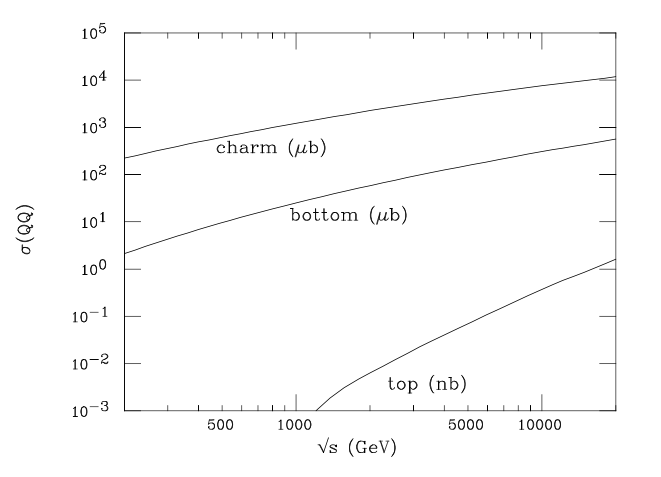
\includegraphics[width=7.6cm]{FigCap2/HQxsecPPcoll.png}
      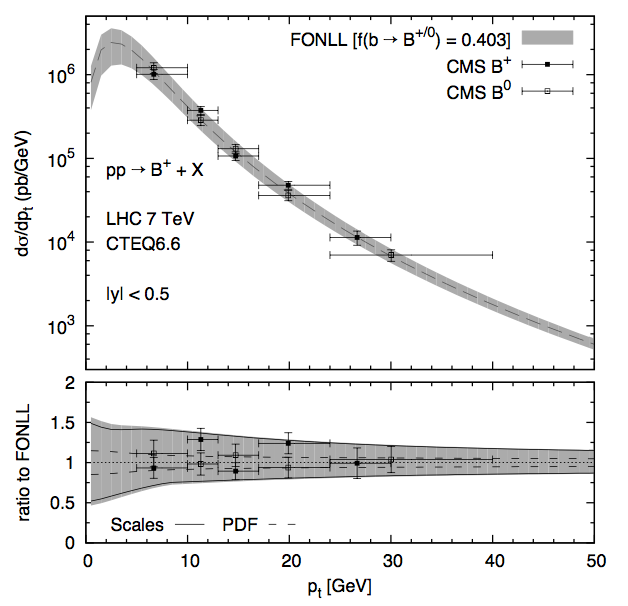
\includegraphics[width=6.4cm]{FigCap2/FONLLBmeson.png}
  \caption{Left: total production cross-sections for charm, bottom and top quark pairs, in pp collisions as a function of the center-of-mass energy~\cite{Mangano:1997ri}. Right: FONLL calculation and systematics band~\cite{Cacciari:2012ny} for beauty-hadron production, rescaled to the $|y| <$ 0.5 region, and comparison with CMS data~\cite{Khachatryan:2011mk,Chatrchyan:2011pw}.}
  \label{fig:HQxsecPPcoll}
\end{figure}
For charm quarks, experimental data for individual D-meson species exist.
Since from the theoretical point of view some differencies are 
expected in the quark fragmentation into 
pseudo-scalar ($\Dzero, \Dplus$) and vector ($\Dstar$) mesons, 
one needs to define two different FF. The functional forms used for
the FF of charm quarks in FONLL are taken from~\cite{Cacciari:2003zu}
and have one single non-perturbative parameter
common to the pseudo-scalar and vector FF. This parameter is adjusted on
ALEPH data~\cite{Barate:1999bg} for $\Dstar$ production.
Fig.~\ref{fig:HQxsecPPcoll} (right) shows the CMS measurement 
of $\pt$-differential cross-section for $B^+$ and $B^0$ mesons
as a function of $\pt$ in the rapidity interval $|y| < 0.5$ in pp collision 
at $\sqrt{s} = 7$ TeV~\cite{Khachatryan:2011mk,Chatrchyan:2011pw}, 
compared to FONLL predictions.
The FONLL uncertainty band is obtained from variations of 
renormalisation scale $\mu$ and common factorisation
scale $\mu_f$ as well as of the heavy-quark mass.
Similar comparison, but for charmed hadrons, is shown in Fig.~\ref{fig:CharmXsec} 
for $\Dzero$-meson production
in pp collision at $\sqrt{s} = 7$ TeV measured by 
ALICE~\cite{Acharya:2017jgo}, as a function of $\pt$. FONLL 
predictions are displayed in the left panel and GM-VFNS in the right one. 
Calculations are in agreement with bottom and charm production 
at the LHC, within their
uncertainties. FONLL central values tend to underestimate charm production, 
that systematically lays on the upper edge of FONLL uncertainty band, 
whereas GM-VFNS tends to slightly overestimate the production 
at high $\pt$ but agrees very well at intermediate-low $\pt$. \\



In contrast to FONLL and GM-VFNS, that are based on NLO 
pQCD calculations and are limited to inclusive production
of heavy quarks and mesons, general-purpose Monte Carlo 
generators, such as PYTHIA~\cite{Sjostrand:2006za}, provide a more complete description 
of the final state, including decay kinematics. They simulate the 
final states of high-energy collisions in full detail, including hard and 
soft interactions, parton distributions, initial- and final-state parton 
showers, multiparton interactions, fragmentation and decay. They contain a large 
list of hard Standard Model and Beyond Standard Model processes, 
which are interfaced with parton emission, different models of hadronisation and particle decays. 
The processes are treated at leading order (LO). The higher order 
calculations are included only in an
approximate approach. However, the next-to-leading order (NLO) 
is needed to compare results with experimental data.
PYTHIA generator, for example, contains 
theoretical perturbative QCD calculations that are exact only
at leading order, where only the pair creation processes 
$q\overline{q} \rightarrow Q\overline{Q}$ and $gg \rightarrow Q\overline{Q}$
are included. Higher-order contributions at the NLO to account 
for flavour excitation processes like $qQ \rightarrow qQ$, $gQ \rightarrow gQ$
and the gluon splitting $g \rightarrow Q\overline{Q}$ are also accounted. 
The cross-section of these processes 
diverges as the transverse momentum of the outgoing quarks of the 
hard interaction ($\pt^{hard}$) goes to zero. 
The divergences can be controlled by a lower cut 
on the value of  $\pt^{hard}$, that has a large influence in the 
heavy-flavour production 
in the low-$\pt$ region, which is of the prime interest for ALICE. 
To compare PYTHIA to data, $\pt^{hard}$ and
other PYTHIA parameters must be tuned to reproduce as well 
as possible NLO predictions.
The first generator of heavy-quark production that did the effort of matching NLO calculations 
with LO calculations was MC@NLO~\cite{Frixione:2002ik}.
It proposed a first solution to the double counting of NLO events, 
by subtracting the approximated 
NLO cross section (which were implemented in the general generators)
 from the exact NLO cross section.
The NLO calculations for the hard processes in heavy-flavour production are obtained within the 
POWHEG~\cite{Frixione:2007nw} (Positive Weight Hardest Emission Generator) method. 

\begin{figure}[!ht]
  \centering
  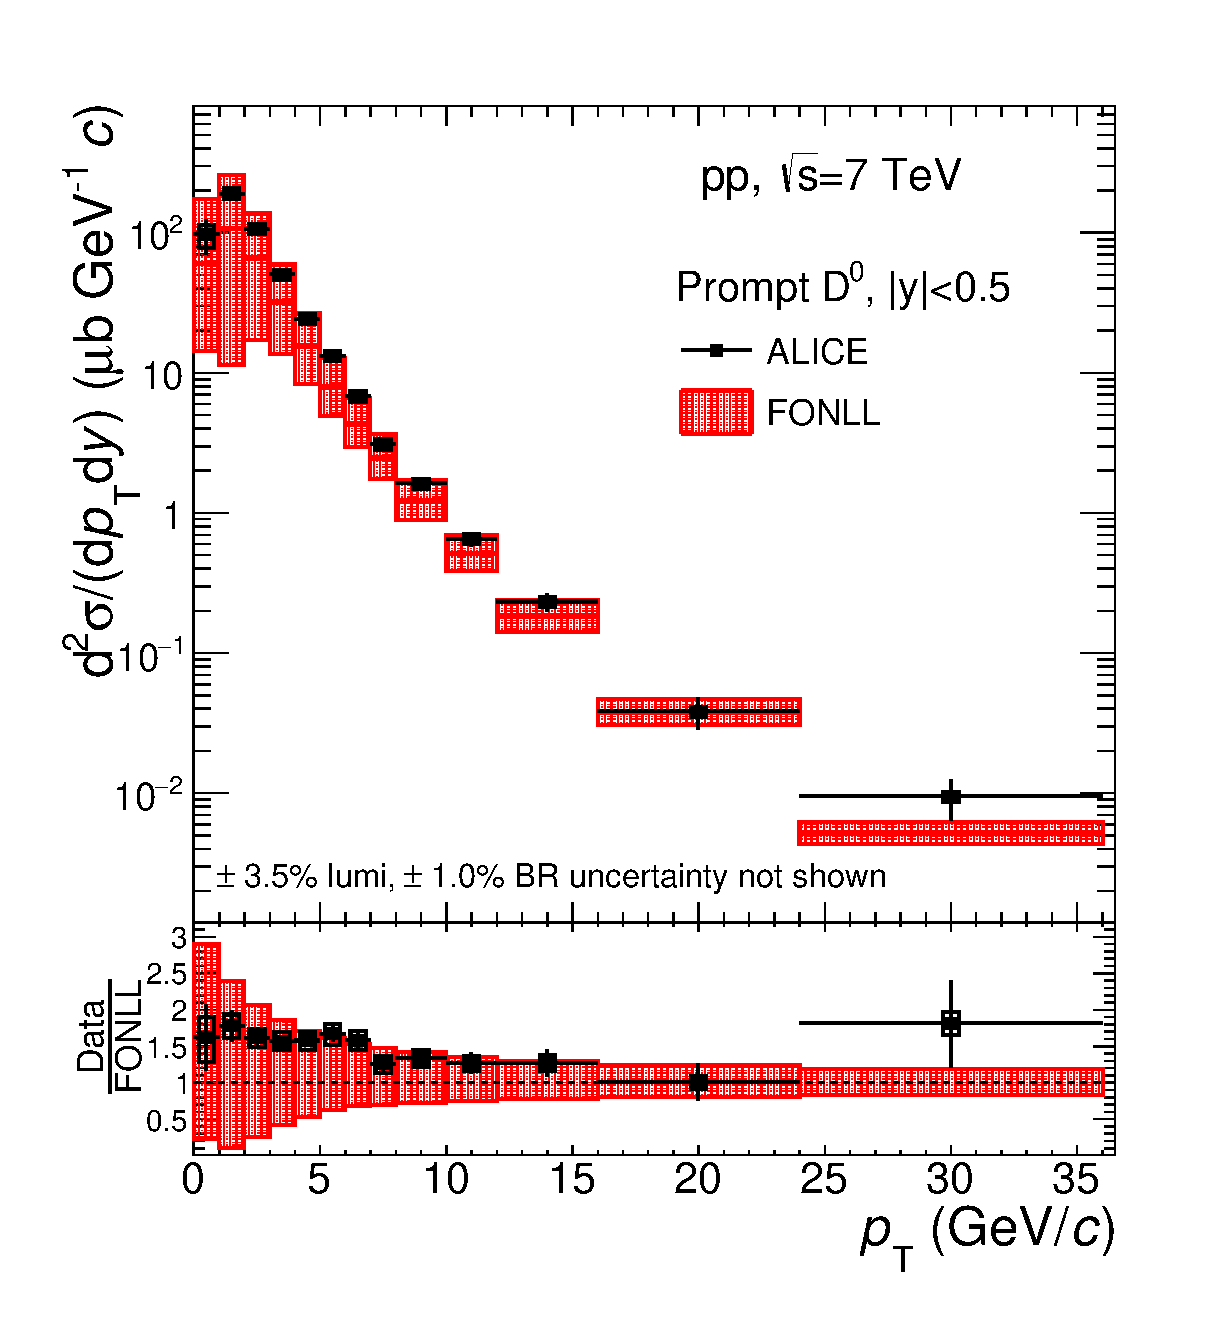
\includegraphics[width=7cm]{FigCap2/DzeroppCrossSecVsFONLLAndRatio.eps}
  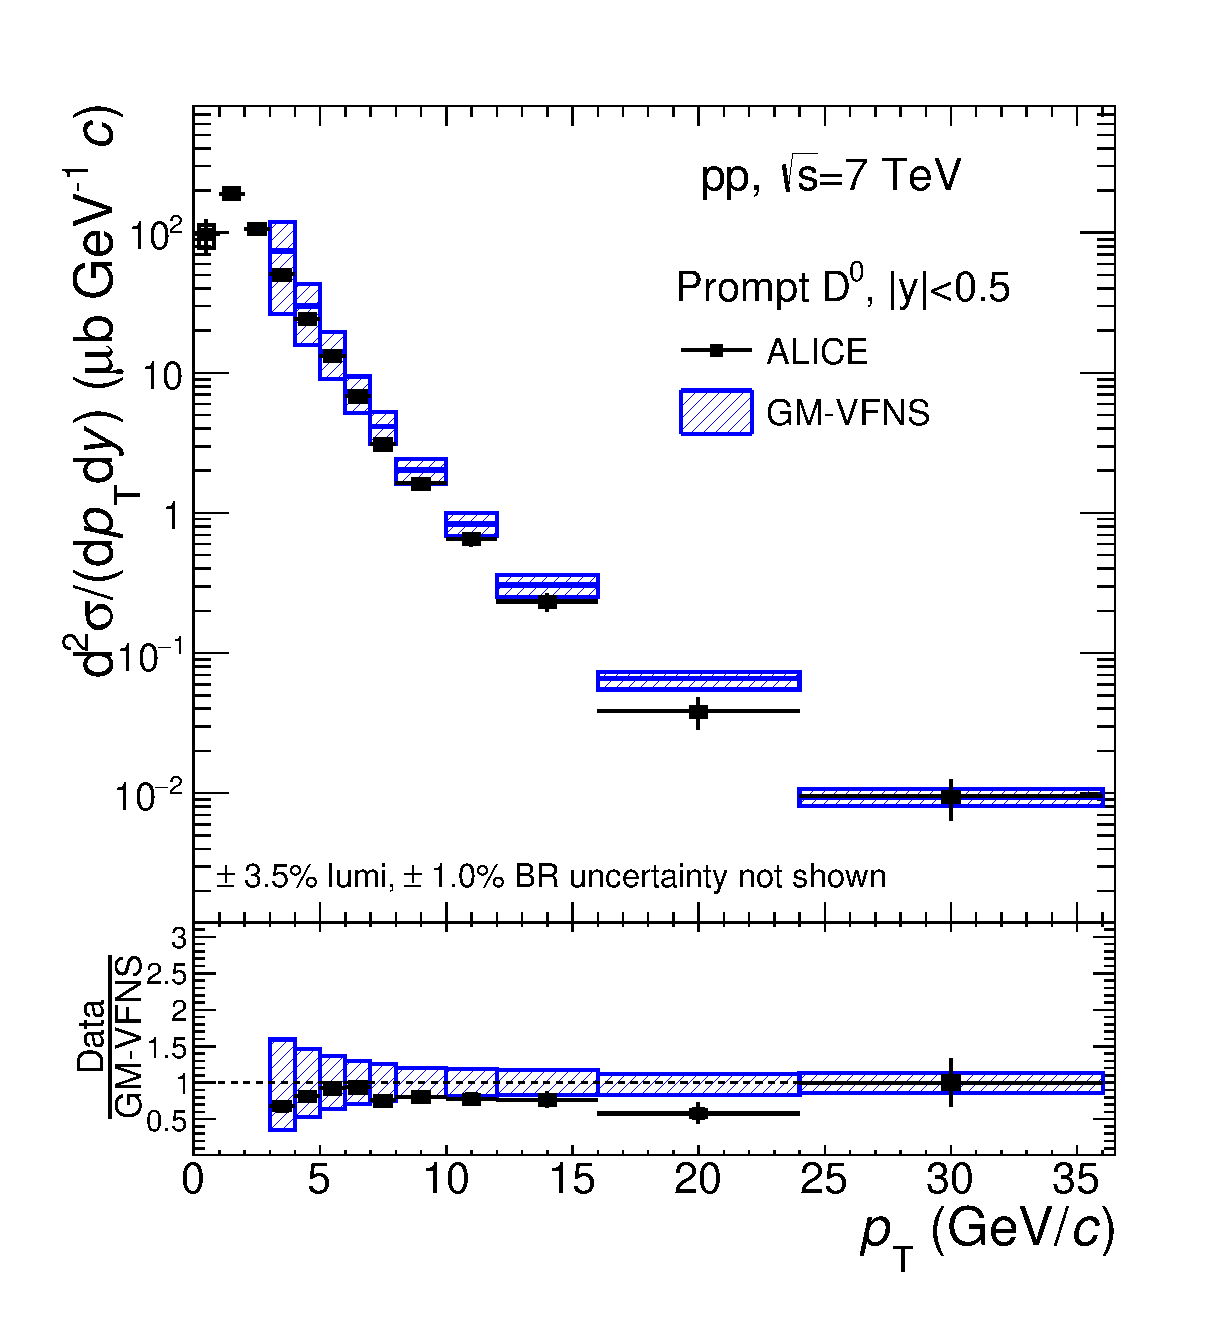
\includegraphics[width=7cm]{FigCap2/DzeroppCrossSecVsGMVFNSAndRatio.eps}
  \caption{$\pt$-differential production cross section of prompt $\Dzero$ mesons with $|y| < $ 0.5 in the interval $0 < \pt < 36 ~\Gevc$, in pp collisions at $\sqrt{s} = 7$ TeV~\cite{Acharya:2017jgo}. The cross section is compared to pQCD calculations: FONLL~\cite{Cacciari:1998it,Cacciari:2001td} (left panel) and GM-VFNS~\cite{Kniehl:2004fy} (right panel).}
  \label{fig:CharmXsec}
\end{figure}

\section{Heavy quarks in p-A collisions}
\label{sec:HFpA}
\subsection{Cold nuclear matter effects}
\label{sec:CNM}
The importance of studying heavy-flavour production in p-A collisions relies on the possibility to
characterise a class of phenomena that are expected to break the binary scaling in 
nucleus-nucleus collisions but are not a consequence of the presence of a 
deconfined plasma. Such effects can in fact be present both in p-A and in A-A collisions and
their origin is mainly related to modification of the PDFs for nucleons bound in nuclei and
multiple soft scatterings of the partons in the nuclei prior to the
hard interaction energy loss in cold nuclear matter. 
They are usually called Cold Nuclear Matter (CNM) effects and
can affect the partons that undergo the hard 
scattering process (initial-state effects) as well as
the produced heavy quarks and hadrons (final-state effects).
Furthermore, recent interest in p-A collisions
is focused on revealing possible effects that could indicate the 
formation of a QGP droplet in small collision systems~\cite{Beraudo:2015wsd,Bozek:2014era,Bzdak:2013zma}.

\subsection{Nuclear Parton Distribution Functions}
\label{sec:nPDFs}
One can quantify the nuclear modification for the parton distribution function via the ratio:
\begin{equation}
\label{eq:RA}
R_i^A(x,Q^2) = f_{i/A}(x,Q^2) / f_{i/p}(x,Q^2)
\end{equation}
\begin{figure}[!ht]
  \centering
  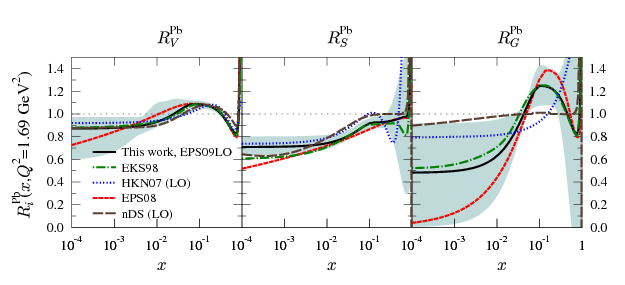
\includegraphics[width=15cm]{FigCap1/PartonNMF.png}
  \caption{The nuclear modification factor (Eq.~\ref{eq:RA}) in a Pb nucleus $R_i^A(x,Q^2)$ for three different flavours as given by the available nPDF parameterizations at LO~\cite{Eskola:2009uj}.}
  \label{fig:nPDF}
\end{figure}
where $f_{i/A}(x,Q^2)$ and $f_{i/p}(x,Q^2)$ are the parton distribution functions in the 
nucleus and in the proton respectively, and the variable $x$ represents the fraction of 
the nucleon momentum carried by a parton. Fig.~\ref{fig:nPDF} 
shows the ratios $R_i^A(x,Q^2)$ for the valence quarks, sea quarks and 
gluons inside a Pb nucleus as obtained from LO global DGLAP 
calculations with EKS98~\cite{Eskola:1998df,Eskola:1998iy}, 
EKPS~\cite{Eskola:2007my},
nDS~\cite{Eskola:2008ca}, HKN07~\cite{Hirai:2007sx} and EPS09LO~\cite{Eskola:2009uj}
parameterisations of the nuclear PDFs which are tuned on measurements
of DIS, Drell-Yan and hadron and dijet production in p-A collisions. 
In general, four different regions are visible in the trend of $R_i^A(x,Q^2)$ versus $x$,
which correspond to four $x$-regimes in which different 
effects influence the PDFs of bound nucleons:
\begin{itemize}
\item {\bf Fermi motion:} this effect is due to the 
thermal momentum that nucleons have inside the nucleus. 
Thus the structure function $F^A_2(x)$ of the bound nucleons
is the convolution of the structure function of the free nucleon 
$F^N_2(x/z)$ (where $z$ is the momentum fraction
of the nucleons times the atomic number of the nucleus) 
with the momentum distribution
of nucleons $f_N(z)$ inside the nucleus: 
$F^A_2(x) = \int_x^A dz f_N(z) F_2^N(x/z)$.
This is the dominant effect for $x > 0.7$.
\item {\bf EMC effect:} first observed in 1982 by EMC collaboration~\cite{Aubert:1983xm},
this effect appears as $R_i^A(x,Q^2)<1$, especially affecting the region 
of valence quarks $0.2 < x < 1$. Fig.~\ref{fig:EMC} left shows the ratio of the structure functions 
of iron $F^{iron}_2(x)$ and deuterium $F^D_2(x)$, that one would expect to be at 1 (except for 
some corrections at high $x$ from Fermi motion). From further
experimental investigations, it was clear that the effect is almost independent from the 
squared momentum transfer, it increases with nuclear mass 
number A and scales approximately with the average nuclear density. 
Many phenomenological models tried to explain such behaviour. 
In the $Q^2$-rescaling models, 
quarks in nuclei move in a larger confinement volume and, 
because of the uncertainty principle, 
they carry less momentum than quarks in free nucleons. 
Some models proposed that 
quarks in nuclei move in quark bags with $n$ quarks, 
other proposed an enhancement 
of pion-cloud effects and a nuclear pionic field, 
but no models so far are universally accepted. 
\iffalse
 In 2009 other pieces of information were added with the
discovery of a strong correlation between the slope of the ratio $R_i^A(x,Q^2)$ in 
the region of EMC effect and the magnitude of the scaling plateau 
at $x > 1$ (see Fig.~\ref{fig:EMC}, right panel)~\cite{Seely:2009gt}.
\fi
\item {\bf Nuclear shadowing and anti-shadowing:} a second depletion region
is observed in the ratio of parton distribution functions $f_{i/A}(x,Q^2) / f_{i/p}(x,Q^2)$ 
at very low $x<0.01$ (typical region of sea quarks). This is commonly denoted 
by shadowing region and is accompanied by
an anti-shadowing region at $0.01 < x < 0.2$ in which the ratio $R_i^A(x,Q^2)$
is above unity.~Different models were
proposed to explain the nuclear shadowing. Some models are based on virtual 
photon fluctuations into vector meson states (GVMD); others
invoke superposition ad fusion of partons of different nucleons at very low $x$, that should deplete the 
region, thus favouring the population of the anti-shadowing region.

\end{itemize}


\begin{figure}[!ht]
  \centering
  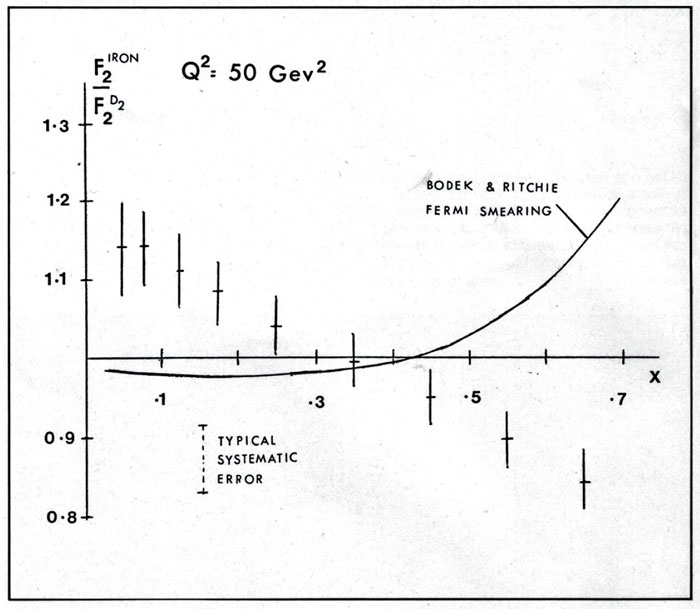
\includegraphics[width=7cm]{FigCap2/EMC.jpg}
%  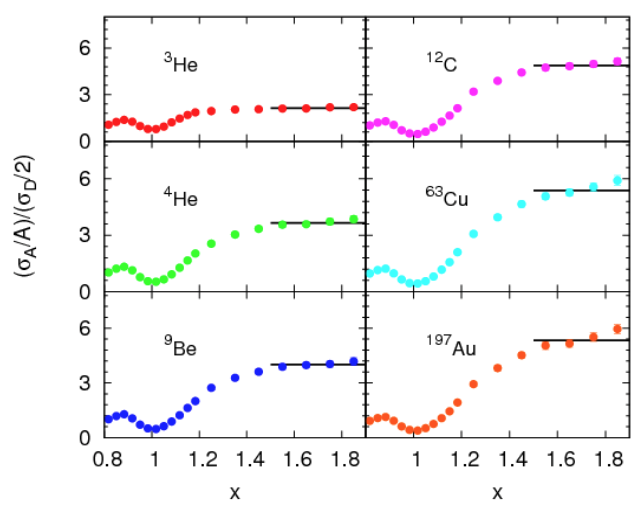
\includegraphics[width=7.5cm]{FigCap2/EMC2.png}
  \caption{Ratio of iron $F^{iron}_2(x)$ and deuterium $F^D_2(x)$ structure function as a function of Bjorken-$x$~\cite{Aubert:1983xm}.% Right: ratio of nucleus $F^{A}_2(x)$ and deuterium $F^D_2(x)$ for different nuclei as a function of Bjorken-$x$~\cite{Seely:2009gt}.
  }
  \label{fig:EMC}
\end{figure}



An other CNM effect is the so-called Cronin Effect~\cite{Cronin:1974zm}, 
discovered in the '70s at FermiLab. It consists in an observed 
enhancement in the nuclear modification factor for $\pt$ 
values between 2 and 5 $\Gevc$. This is commonly understood as due to 
the fact that, in p-A collisions, the 
partons of the projectile nucleon undergo several elastic 
scatterings with the partons of the target nucleus before the hard scattering process 
occurs. The multiple scatterings give the parton an extra 
momentum component in the transverse plane ($k_{\rm T}$ broadening), 
which causes a broadening of the $\pt$ spectra of the heavy 
quarks produced in the hard scattering processes,  
resulting in an enhancement of the nuclear modification factor at 
low and intermediate $\pt$. Going towards 
larger values of transverse momentum, the extra-$k_{\rm T}$ 
from the elastic collisions becomes negligible and the nuclear 
modification factor gets close to unity.\\
%The x regime relevant for charm production at the LHC ($\sim 10^{-4}$ ) is about 2 orders of magnitude lower than at RHIC and 3 orders of magnitude lower than at the SPS [43]. In this region with low x-values, modifications of the nuclear PDFs are mainly related to the shadowing effect.
\begin{figure}[!ht]
  \centering
  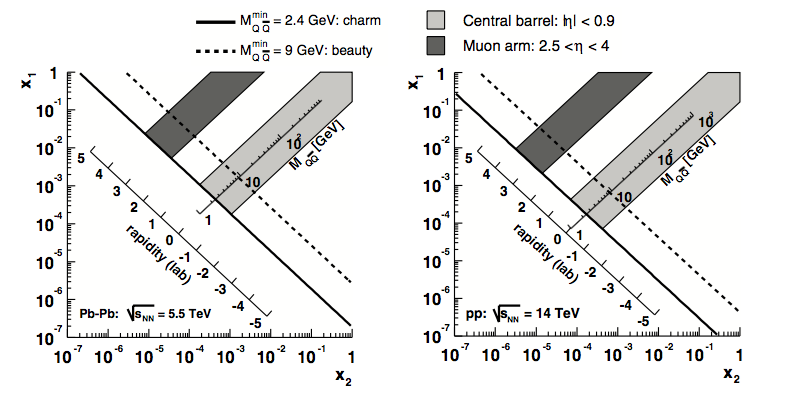
\includegraphics[width=15cm]{FigCap2/xBjork.png}
  \caption{ALICE acceptance in the ($x_1, x_2$) plane for heavy flavours in Pb-Pb at $\sNN = 5$ TeV on the left panel and pp collisions at $\sqrt{s} = 14$ TeV on the right~\cite{Alessandro:2006yt}. }
  \label{fig:xBjork}
\end{figure}



Let's turn now to understand which are the ranges of Bjorken $x$
at play when producing $c\overline{c}$ and $b\overline{b}$ pairs at the LHC. 
The probed $x$ value depends on the center-of-mass energy
of the collision, on the invariant mass $M_{Q\overline{Q}}$ of the 
$Q\overline{Q}$ pair produced in the hard scattering
and on its rapidity $y_{Q\overline{Q}}$. Under the hypothesis 
that the transverse momentum of the parton 
in the nucleon is negligible, the four-momenta of the two 
incoming gluons are $(x_1,0,0,x_1)\cdot(Z_1/A_1)\sqrt{s_{\rm pp}}/2$
and $(x_2,0,0,-x_2)\cdot(Z_2/A_2)\sqrt{s_{\rm pp}}/2$, where 
$x_1$ and $x_2$ are the momentum fractions 
carried by the gluons, and $\sqrt{s_{\rm pp}}$ is the c.m.s. energy for pp collisions,
that differs from the c.m.s $\sNN$ energy of colliding nuclei by the factor $Z/A$. 
The square of the invariant mass of the produced $Q\overline{Q}$ pair is given by:
\begin{equation}
\label{eq:Mqq}
M_{Q\overline{Q}}^2 =  x_1 x_2 s_{\rm NN} = x_1 \frac{Z_1}{A_1} x_2 \frac{Z_2}{A_2} s_{\rm pp},
\end{equation}
and the rapidity in the laboratory is:
\begin{equation}
\label{eq:yqq}
y_{Q\overline{Q}} = \frac{1}{2} {\rm ln} {\Big [ } \frac{E +p_z}{E-p_z}  {\Big ] }= \frac{1}{2} {\rm ln} {\Big [ } \frac{x_1}{x_2} \cdot \frac{Z_1 A_2}{Z_2 A_1} {\Big ] }.    
\end{equation}
From Eq.~\ref{eq:Mqq} and~\ref{eq:yqq} and for a symmetric colliding system $(A_1 = A_2, Z_1 = Z_2)$
one obtains:
\begin{equation}
\label{eq:x1x2}
x_1 = \frac{M_{Q\overline{Q}}}{\sqrt{s_{\rm NN}}} {\rm exp} (+y_{Q\overline{Q}} ), \; \; \; \; \; \;
x_2 = \frac{M_{Q\overline{Q}}}{\sqrt{s_{\rm NN}}} {\rm exp} (-y_{Q\overline{Q}} ). 
\end{equation}\\




Because of its lower mass, charm allows to probe lower $x$ values than beauty. 
The $x$ regime relevant for charm production at the LHC ($\approx 10^{-4}$) is about 
2 orders of magnitude lower than at RHIC and 3 orders of magnitude lower than at the SPS.
Measurements of charm and beauty particles in the forward (or backward) rapidity region ($|y| \sim 4 $) 
gives access to $x$ regimes about 2 orders of magnitude lower, down to $x \approx 10^{-6}$.
Fig.~\ref{fig:xBjork}~\cite{Alessandro:2006yt} shows the ($x_1, x_2$) 
plane for charm and bottom production at the LHC
covered by the ALICE acceptance, for Pb-Pb
collisions at $\sNN = 5$ TeV on the left panel and pp collisions 
at $\sqrt{s} = 14$ TeV on the right.
The shadowed regions correspond to the rapidity region covered 
by the ALICE central barrel ($|\eta| < 0.9$) and by the 
muon arm ($-4 < \eta < -2.5$).
The points with equal invariant mass ($c\overline{c}$ and $b\overline{b}$ pairs) lie on hyperbolae (straight lines in the log-log scale).\\


\subsection{Experimental results in p-A collisions}
\label{sec:HFresultspA}
The nuclear modification of the PDFs can significantly affect final hadrons yields,
especially at low $\pt$ due to shadowing, which is the most relevant effect at LHC energies.
One can define the nuclear modification factor for p-Pb collisions as:
\begin{equation}
R_{\rm pPb} = \frac{1}{A}\frac{d^2\sigma_{pPb}^{\rm prompt D}/d\pt dy}{d^2\sigma_{pp}^{\rm prompt D}/d\pt dy},
\end{equation}
where A is the Pb mass number $A = 208$. \\
\begin{figure}[!ht]
  \centering
  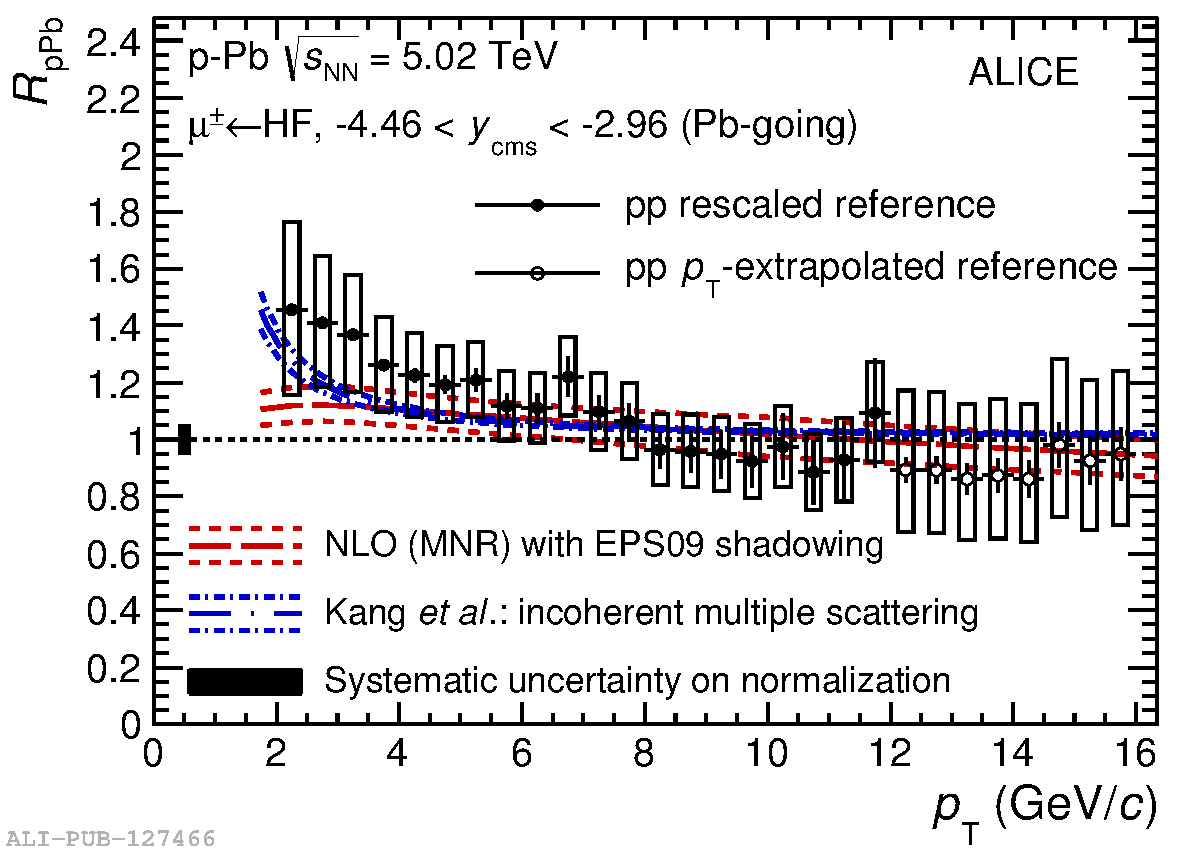
\includegraphics[width=7cm]{FigCap2/2017-Feb-05-Fig2b.pdf}
  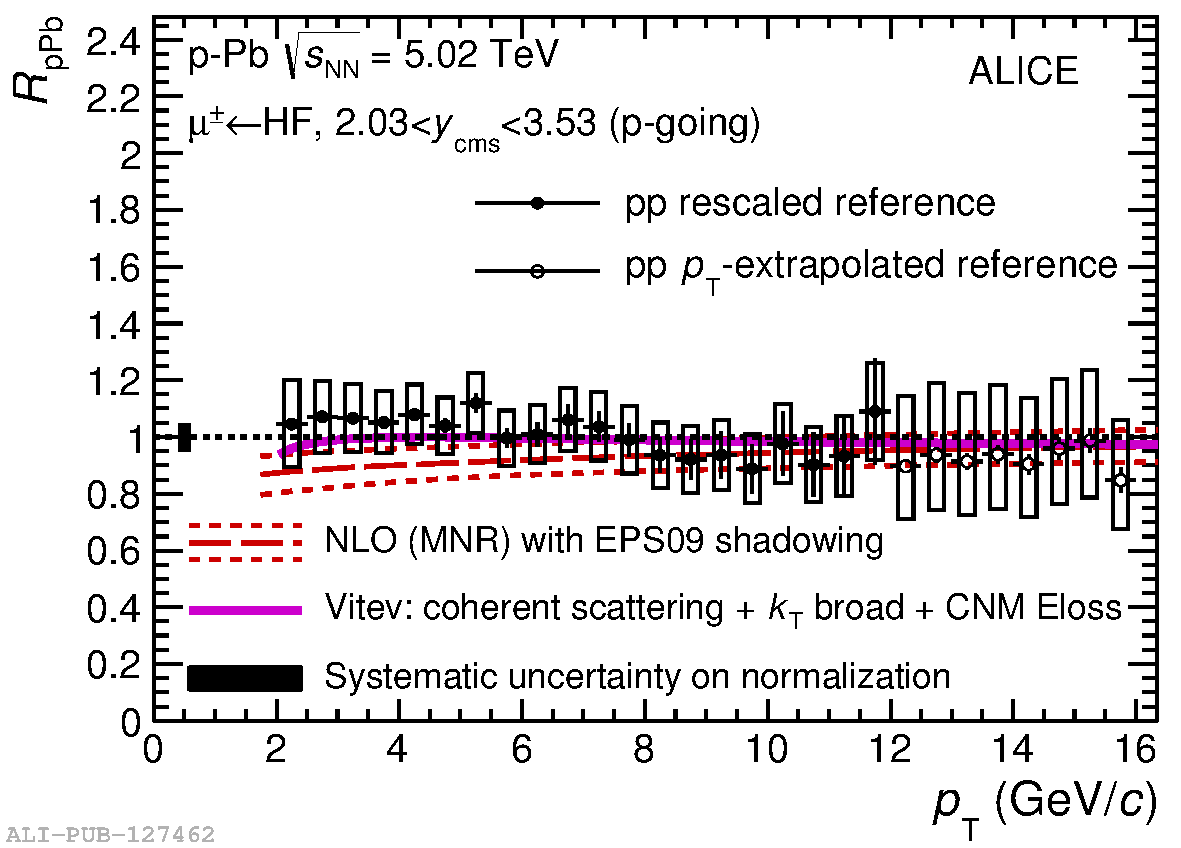
\includegraphics[width=7cm]{FigCap2/2017-Feb-05-Fig2a.pdf}
  \caption{Nuclear modification factor of muons from heavy-flavour hadron decays as a function of $\pt$ for p-Pb collisions at $\sNN = 5.02$ TeV at backward rapidity ($4.46 < y_{\rm cms} < 2.96$, left) and forward rapidity ($2.03 < y_{\rm cms} < 3.53$, right)~\cite{Acharya:2017hdv} compared to model predictions~\cite{Kang:2014hha,Mangano:1991jk}. }
  \label{fig:muons}
\end{figure}
\begin{figure}[!ht]
  \centering
    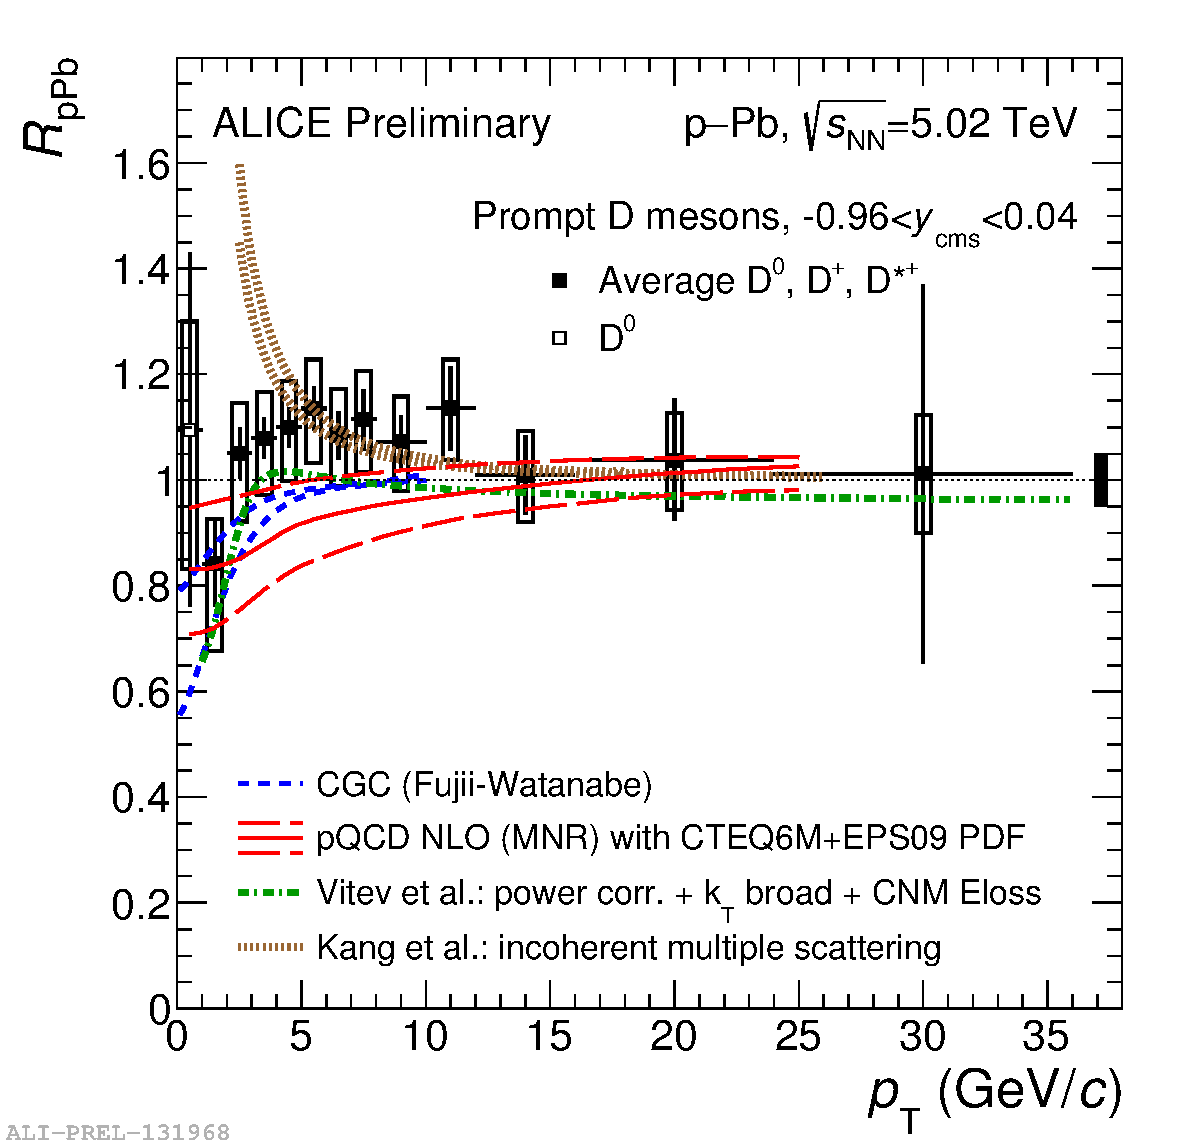
\includegraphics[width=7cm]{FigCap2/2017-Jul-05-pPbWithModelsCNM.pdf}
    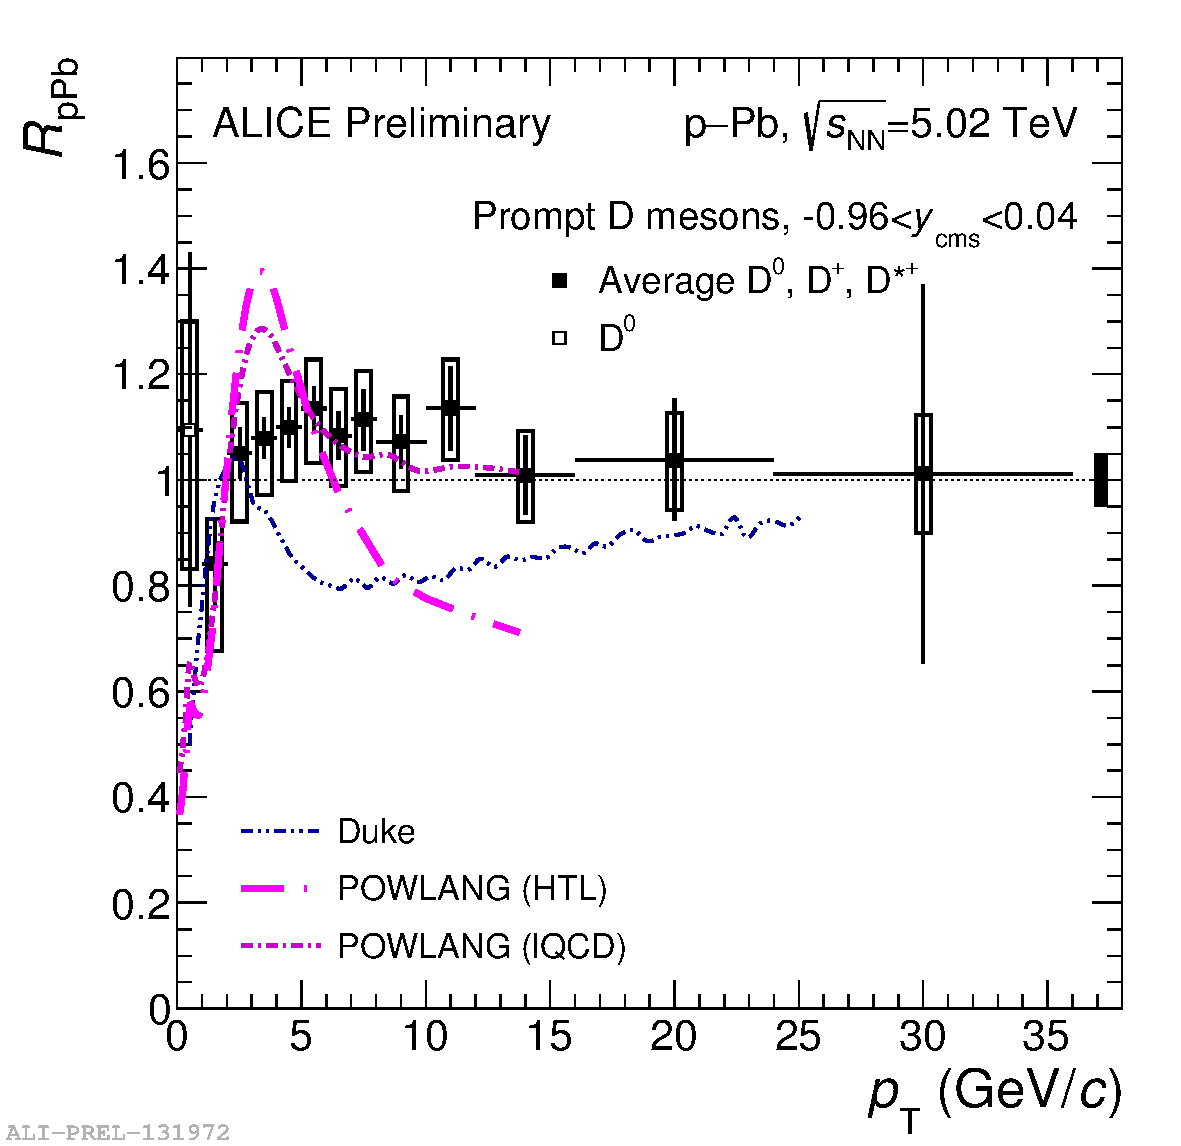
\includegraphics[width=7cm]{FigCap2/pPbWithModelsMedium.pdf}
  \caption{Left: nuclear modification factor $R_{\rm pPb}$ of prompt D mesons in p-Pb collisions at $\sNN = 5.02$ TeV. Data are compared with results of theoretical calculations including only CNM effects~\cite{Fujii:2017rqa,Cacciari:2012ny,Eskola:2016oht,Sharma:2009hn,Kang:2014hha}. Right: the results of the Duke~\cite{Xu:2015iha} and POWLANG~\cite{Beraudo:2015wsd} transport models are compared with the measured D-meson $\RpPb$.}
  \label{fig:RpA}
\end{figure}


ALICE measured the $\pt$-differential nuclear modification factor 
$R_{\rm pPb}$ of muons from heavy-flavour hadron decays in p-Pb collisions at $\sNN = 5.02$ TeV
at forward and backward rapidity~\cite{Acharya:2017hdv} (Fig.~\ref{fig:muons}).
While at forward rapidity muon $R_{\rm pPb}$ is compatible 
with unity in the full $\pt$ range ($2 <\pt < 16 \, \Gevc$) in which the 
measurement was carried out, 
at backward rapidity, it is larger than unity at low $\pt$ with a maximum 
deviation of $R_{\rm pPb}=1$ of 2.2$\sigma$ of the combined statistical and 
systematic uncertainties in the interval $2.5 < \pt < 3.5 \;\Gevc$. 
At higher $\pt$, it is compatible with unity. The results indicate
that CNM effects are small and that the strong suppression of the
yields of muons from heavy-flavour hadron decays observed in the
10\% most central Pb-Pb collisions~\cite{Abelev:2012qh} should result from final-state
effects, i.e. the heavy-quark in-medium energy loss. 
ALICE also measured the $R_{\rm pPb}$ of prompt 
D mesons in p-Pb collisions at $\sNN = 5.02$ TeV
as a function of $\pt$ and the results are shown in 
Fig.~\ref{fig:RpA} (left panel)~\cite{ALICEPAS2017008}. 
Data are compared to theoretical models that include CNM effects: 
a calculation based on the Color Glass Condensate
formalism~\cite{Fujii:2013yja,Fujii:2017rqa}, a FONLL 
calculation~\cite{Cacciari:2012ny} with CTEQ6M PDFs~\cite{Pumplin:2002vw} 
and EPPS16 NLO nuclear modification~\cite{Eskola:2016oht}, 
a LO pQCD calculation with intrinsic $k_{\rm T}$ broadening, 
nuclear shadowing and energy loss of the charm quarks 
in cold nuclear matter (Vitev et al.)~\cite{Sharma:2009hn}, 
and a higher-twist calculation based on incoherent multiple 
scatterings (Kang et al.)~\cite{Kang:2014hha}. 
The three former calculations describe the data within 
uncertainties in the entire $\pt$ range, although for the CGC 
calculation the compatibility with the data 
in 3-12 $\Gevc$ is at the limit of the uncertainties of the data 
and of the calculations. The calculation by Kang et al., which has 
a different trend with respect to the others, is disfavoured by the 
data for $\pt<3$--$4~\gev/c$.
CNM effects are expected to be largest for small $\pt$, where, in 
addition, the predictions of the different theoretical approaches differ 
and the statistical uncertainty of the present measurement for the 
lowest $\pt$ interval is about 30\% and does not 
discriminate the different models.
In the right-hand panel of Fig.~\ref{fig:RpA}, the data are 
compared with the results of two transport model 
calculations, Duke~\cite{Xu:2015iha} and 
POWLANG~\cite{Beraudo:2015wsd}, both of them assuming that a 
Quark--Gluon Plasma is formed in p--Pb collisions.
Both models are based on the Langevin approach for the transport of heavy 
quarks through an expanding deconfined medium described by relativistic viscous 
hydrodynamics. In both the Duke and POWLANG results the D-meson nuclear modification
factor shows  a structure with a 
maximum at $\pt \approx 2.5~\Gevc$, possibly followed by a moderate 
($<20$-30\%) suppression at higher $\pt$,
resulting from the interplay of CNM effects and interactions of charm quarks with the
radially expanding medium.
The trend predicted by these models is disfavoured by the data, which in particular 
disfavour a suppression 
larger than 10-15\% in the interval $3<\pt<12~\Gevc$.\\
\begin{figure}[!ht]
  \centering
    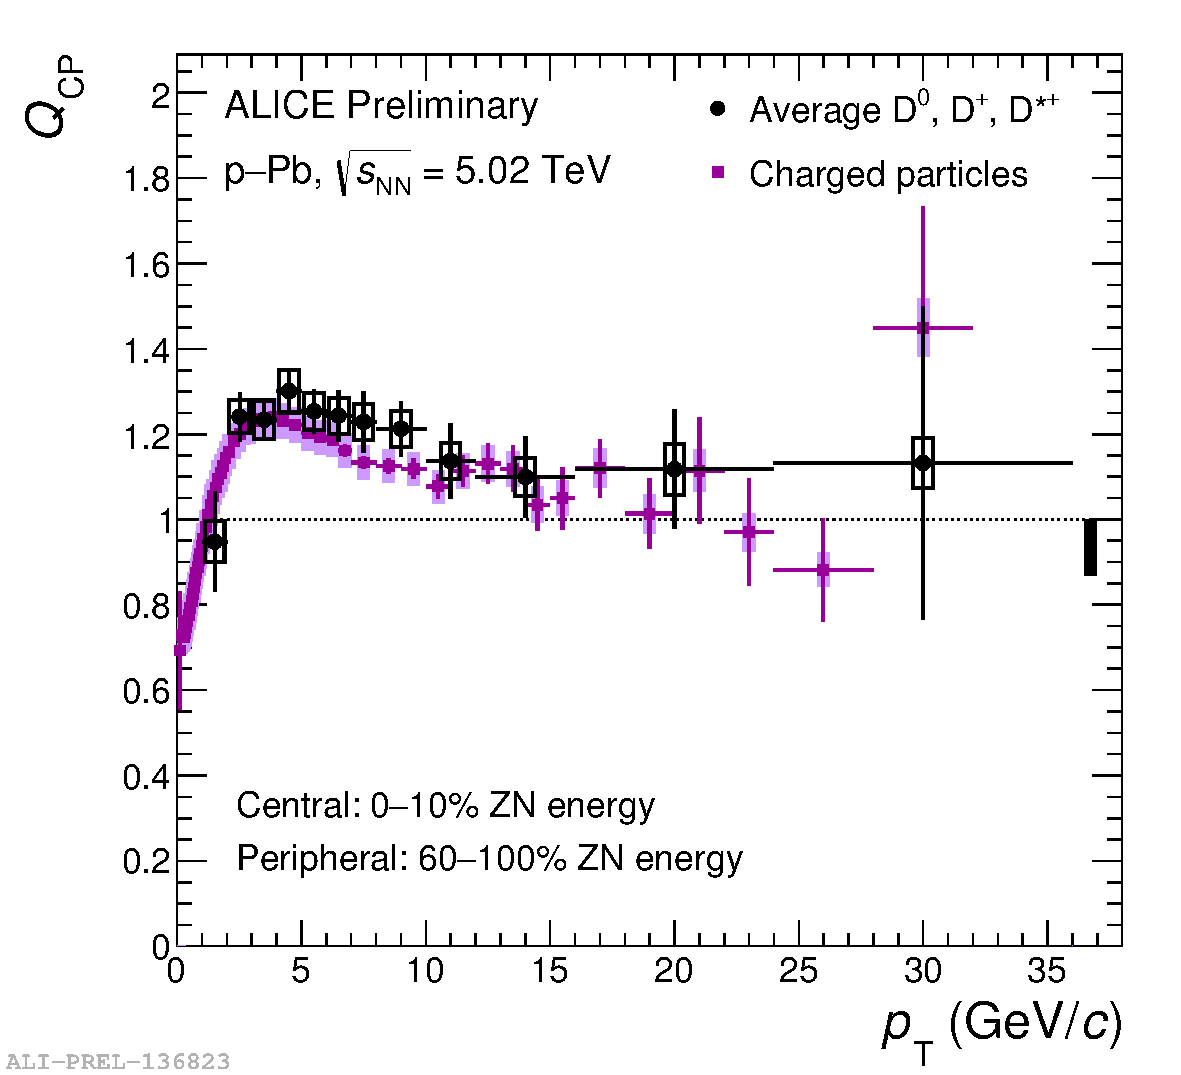
\includegraphics[width=8cm]{FigCap2/2017-Sep-12-QCP-Daverage-ChargedHadrons.pdf}
  \caption{D-meson (black) and charged-particle (magenta) central-to-peripheral nuclear modification factor~\cite{ALICEPAS2017008}.}
  \label{fig:RpA}
\end{figure}




The nuclear modification factor in p-Pb collisions can be also measured in given centrality classes.
Its definition is:
\begin{equation}
Q_{\rm pPb}^{\rm mult} = \frac{({\rm d}^2 N/{\rm d} \pt {\rm d} y)^{\rm mult}_{\rm pPb}}{\langle T_{\rm pPb} \rangle ^{\rm mult}({\rm d}^2 \sigma_{pp}/{\rm d} \pt {\rm d} y)},
\end{equation}
where $({\rm d}^2 N/{\rm d} \pt {\rm d} y)^{\rm mult}_{\rm pPb}$ 
is the yield of a given species in p-Pb collisions 
in a given centrality class, and $\langle T_{\rm pPb} \rangle ^{\rm mult}$ is the average nuclear 
overlap function in the same centrality class.
In order to achieve better precision on the yields, the ratio of the nuclear 
modification factor in central to peripheral events, $Q_{\rm CP}$, 
can be defined as:
\begin{equation}
Q_{\rm CP} = \frac{({\rm d}^2 N/{\rm d} \pt {\rm d} y)^{\rm central}_{\rm pPb}/ \langle T_{\rm pPb} \rangle^{\rm central}}{({\rm d}^2 N/{\rm d} \pt {\rm d} y)^{\rm peripheral}_{\rm pPb}/ \langle T_{\rm pPb} \rangle^{\rm peripheral}}.
\label{eq:QCP}
\end{equation}
The $Q_{\rm CP}$ of D mesons in the 0-10\% and 60-80\% 
centrality classes was measured by 
ALICE~\cite{ALICEPAS2017008} (Fig.~\ref{fig:RpA}, right panel) 
and it increases in the interval 1-4 $\Gevc$, 
up to values of about 1.25 and then tends to decrease. The 
average value of the D-meson $Q_{\rm CP}$ 
in the interval $3 < \pt < 8 \; \Gevc$ is larger than unity by 1.5 
standard deviations of the combined statistical and systematic uncertainty.
It is an open question whether the observed bump of $Q_{\rm CP}$, whose magnitude is similar 
for D mesons and charged particles, is related to initial state effects 
or to collectivity effects in the final state.
\iffalse
\begin{figure}[!ht]
  \centering
  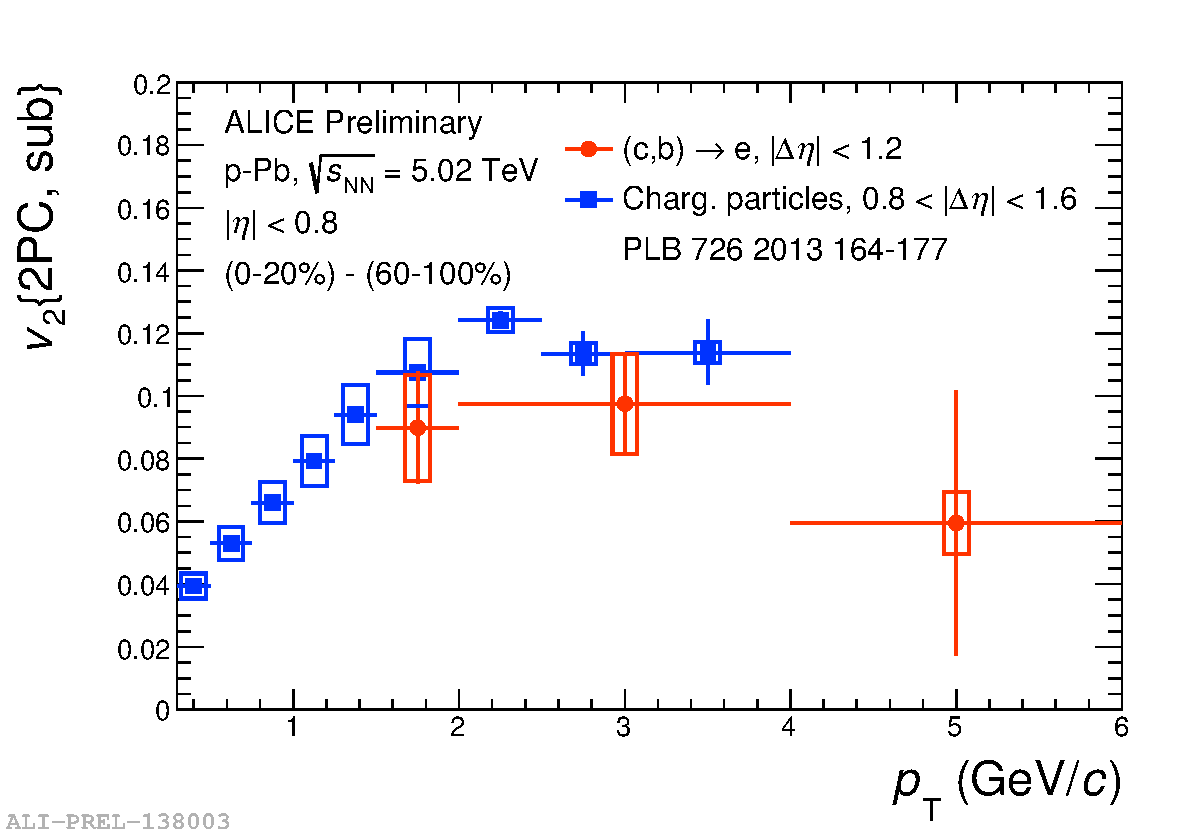
\includegraphics[width=7cm]{FigCap2/v2HFE.pdf}
  \caption{~\cite{Acharya:2017hdv}}
  \label{fig:}
\end{figure}
\fi
\section{Heavy quarks in A-A collisions}
\label{sec:HFEnLossinAA}
High-momentum partons traversing the QGP are expected 
to lose energy because of interactions 
with the medium constituents. One of the experimental observables 
used for the study of energy loss is the 
nuclear modification factor, defined in Sec.~\ref{sec:JetQuenching}. 
The possibility to disentangle
effects of cold nuclear matter from the ones related to in-medium 
energy loss paves the way to characterise the 
hot and dense medium properties. In fact, the magnitude of energy lost in the medium is
determined by the properties of the fireball like the transport coefficients,
that encode the momentum transfers with the medium, or the mean free 
path, closely related to the medium density $\rho$
and the cross section $\sigma$ of the parton-medium interaction. 
A colour charge can lose energy in a plasma at a temperature $T$ by two mechanisms: 
radiative and collisional energy losses, which originate, respectively, from elastic
and inelastic interactions with the medium constituents.
\subsection{Collisional processes}
\label{sec:coll}
Collisional processes are $2 \rightarrow 2$ elastic scatterings off thermal 
gluons (Fig.~\ref{fig:LoopCollScatt}, first to third diagrams) and quarks 
(Fig.~\ref{fig:LoopCollScatt}, fourth diagram). It is possible to calculate,
 in the limit $E \gg M^2/T$, the heavy-quark collisional energy loss 
 ${\rm d} E/{\rm d} x$ in a QGP, by summing all contributions of 
 Fig.~\ref{fig:LoopCollScatt}~\cite{Peigne:2008nd}:
\begin{equation}
\label{eq:QCDenLossColl}
\begin{split}
\frac{{\rm d} E}{{\rm d} x} = \; & \frac{4 \pi T^2}{3}\;  \alpha_s (m^2_D)\;  \alpha_s(ET) {\Big [} {\Big (}  1 + \frac{n_f}{6}{\Big )} {\rm ln} \frac{ET}{m^2_D} + \frac{2}{9} \frac{\alpha_s(M^2)}{\alpha_s(m^2_D)} \times {\rm ln} \frac{ET}{M^2}  \\+\;  &c(n_f) + \mathcal{O}{\Big (}\alpha_s (m^2_D) \; {\rm ln}\frac{ET}{m^2_D}{\Big )}{\Big ]},
\end{split}
\end{equation}
where $\alpha_s$ is the QCD running coupling constant, $n_f$ is the number of flavours 
considered in the scattering diagrams of Fig.~\ref{fig:LoopCollScatt} and $m_D$ is the 
Debye screening mass of the plasma $m_D = 4\pi \alpha_s T^2 (1 + n_f/6)$. 
\begin{figure}[!ht]
  \centering
  \includegraphics[width=14cm]{FigCap2/LO_HQscattering.png}
  \caption{Feynman diagrams for leading-order perturbative HQ scattering off light partons.}
  \label{fig:LoopCollScatt}
\end{figure}

The multiple scatterings of the heavy quark with the medium 
partons can also be treated as Brownian motion and is typically
be described by the Boltzmann equation. In the limit of small 
momentum transfer, the latter can be reduced to the 
Fokker-Planck equation, which is often further reduced into the
Langevin equation. These
partial-differential equations can be used as transport equations, 
to describe the evolution of the momentum distribution
of heavy quarks along time. The Langevin equation for heavy-quark 
collisional energy loss presents itself as~\cite{Cao:2013ita}:
\begin{equation}
\label{eq:Langevin}
\frac{{\rm d} {\vec{p}}}{{\rm d} t} = - \eta_D (p) \vec{p} + \vec{\xi}.
\end{equation}
In Eq.~\ref{eq:Langevin}, the first right-hand side term is the 
deterministic friction force, while the second one is the thermal random noise,
satisfying the properties:
\begin{equation}
\label{eq:Langevin2}
\langle {\xi^i (\pt)} {\xi^j (p_{\rm T'})} \rangle = b^{ij} (\pt) \frac{\delta_{tt'}}{{\rm d} t}, \; \; \; \; b^{ij} (\pt) = k_{\parallel}(p)\hat{p}^i\hat{p}^j + k_{\perp} (\delta^{ij} - \hat{p}^i\hat{p}^j).
\end{equation}
In Eq.~\ref{eq:Langevin2}, $k$ represents the momentum-space 
diffusion coefficient of heavy quarks;
the coefficient $\eta_D$ of Eq.~\ref{eq:Langevin2} is involved in the definition of the spatial 
diffusion coefficient $D_s$, which is related to the momentum-space 
diffusion coefficient via: 
\begin{equation}
\label{eq:Langevin3}
D_s = \frac{T}{M \eta_D} = \frac{2 T^2}{k}.
\end{equation}
To simulate the evolution of heavy quarks, one needs to discretise terms and calculate the increment 
$\vec{p}(t + \Delta t) -  \vec{p}(t)$ at a given time $t$. 

\subsection{Gluon-radiation processes}
\label{sec:rad}
While a parton is traversing the medium, it picks up some transverse 
momentum $k_{\perp}$ due to multiple scatterings. 
If we consider a gluon in the hard parton wave function, when the 
accumulated $k_{\perp}$ is enough, it can decohere from the partonic projectile and be emitted.
These are $1 \rightarrow 2$ processes, like $Q \rightarrow g\, Q$, 
where $Q$ is the heavy quark and $g$ the gluon.
The average phase $\phi$ of the gluon is approximately:
\begin{equation}
\label{eq:gluonPhase}
\phi = {\Big \langle} \frac{k_{\perp}^2}{2\omega} \Delta z {\Big \rangle} \sim \frac{\hat{q} L}{2 \omega} L = \frac{\omega_c}{\omega},
\end{equation}
where $\hat{q}$ is the transport coefficient of the medium, 
defined as the average squared transverse 
momentum transferred to the projectile per average unit path 
length $L$: $\hat{q} = \langle k_{\perp}^2 \rangle / L$ \cite{Salgado:2003gb,}.
Hence, gluons are emitted from the parton traversing a finite path 
length $L$ with a characteristic gluon frequency $\omega_c$:
\begin{equation}
\label{eq:gluonPhase}
\omega_c = \frac{1}{2} \hat{q} L^2.
\end{equation}
The distribution of energy $\omega$ of the radiated gluons, 
for small energies $\omega < \omega_c$ is of the form:
\begin{equation}
\label{eq:gluonEnDistrb}
\omega \frac{{\rm d} I}{{\rm d} \omega} \sim \frac{2 \alpha_s C_R}{\pi} \sqrt{ \frac{\omega_c}{2 \omega}},
\end{equation}
where $C_R$ is the Casimir factor for the QCD coupling, 
equal to 4/3 for quark-gluon coupling and to 3 for gluon-gluon coupling.
The $\omega$-integrated average parton energy loss results then:
\begin{equation}
\label{eq:RadEnLoss}
\langle \Delta E \rangle \propto \alpha_s \, C_R \, \hat{q} \, L^2. 
\end{equation}
We can then summarise the main properties of average parton 
energy loss via radiative processes:
\begin{itemize}
\item it grows with the path length like: $\Delta E \propto L^2$;
\item is proportional to $\alpha_s C_R$, thus it is larger by a factor 
9/4 $ = 2.25$ for a gluon traversing the medium than for a quark;
\item it is independent of the initial parton energy $E$.
\end{itemize}
Furthermore, while in the limit of massless partons the probability of 
gluon emission is maximum for collinear radiation,
in the massive limit the soft-gluon emission probability, for small 
emission angles $\Theta \ll 1$, is~\cite{Dokshitzer:1991fd}:
\begin{equation}
\label{eq:DeadCone}
{\rm d} \sigma_{Q \rightarrow gQ } \sim \frac{\Theta^2 {\rm d} \Theta^2}{[\Theta^2+ \Theta^2_0]} \frac{{\rm d} \omega}{\omega},
\end{equation}
with $\Theta_0 = M_Q/E_Q$.
Therefore, in the kinematical region $\Theta < \Theta_0$ the yield of radiated gluons
in the forward direction provides a small contribution to the total multiplicity. 
The depleted forward region is called the {\it dead cone}.
Since $\Theta_0 = M_Q/E_Q$, the effect is expected to be more 
relevant with increasing parton mass. A hierarchy in 
the energy loss is hence expected:
\begin{equation}
\label{eq:HierachyRaa}
\Delta E_{gluon} < \Delta E_{light\, quark} < \Delta E_{heavy\, quark},
\end{equation}
where the first inequality comes from the different couplings in $gg$ and $gq$ 
processes due to the Casimir factor in Eq.~\ref{eq:gluonEnDistrb} 
and the second from the dead-cone effect. The hierarchy, if present, 
should consequently affect the $\RAA$ values of hadrons originating from
gluon, light and heavy-quark fragmentation.\\


\begin{figure}[!ht]
  \centering
  \includegraphics[width=7cm]{FigCap2/HFEnLoss1.png}
  \includegraphics[width=7cm]{FigCap2/HFEnLoss2.png}
  \caption{Comparison of radiative and collisional energy losses for charm (left) and for bottom (right) quarks from calculations in~\cite{Cao:2013ita}.}
  \label{fig:HFEnLoss}
\end{figure}
In Fig.~\ref{fig:HFEnLoss}, an example of calculations from~\cite{Cao:2013ita}
for the energy loss of charm (left) and beauty (right) quarks 
in central Pb-Pb collisions at the LHC is shown as a function of the initial energy of the quark.
In the model~\cite{Cao:2013ita}, quarks evolve in a static medium at a temperature
$T = 300$ MeV according to a Langevin equation (like that in Eq.~\ref{eq:Langevin}) with 
an additional term for radiative contribution. 
Both the contributions from collisional and radiative energy loss 
are displayed in Fig.~\ref{fig:HFEnLoss}. Elastic interactions
dominate the low-$\pt$ region, up to $\sim 6\; \Gevc$ for charm and $\sim 16 \;\Gevc$ for beauty quarks.
At higher $\pt$, the contribution from radiative processes is the dominant one and must be considered when 
performing calculations at LHC energies.
It is also interesting to look at Fig.~\ref{fig:HFEnLoss2} (left), always from the
same calculations~\cite{Cao:2013ita}, that shows the 
thermalisation process of charm quarks in the medium as a function of time.
The initial energy of the charm quarks is 10 GeV. Depending on the different implementation for energy
loss, the thermalisation of the charm quarks occurs at different times.\\
\begin{figure}[!ht]
  \centering
  \includegraphics[width=7cm]{FigCap2/HFEnLoss3.png}
  \includegraphics[width=7cm]{FigCap2/FragHQ.png}
  \caption{Left: thermalization process of charm quarks in a static medium~\cite{Cao:2013ita}. Right: relative contributions from different hadronisation mechanisms to D-meson production  from charm quarks, as a function of the transverse momentum, from calculations in~\cite{Cao:2013ita}.}
  \label{fig:HFEnLoss2}
\end{figure}

\subsection{Heavy flavour hadronisation in the medium}
\label{sec:HFhadro}

The final hadron yields and momentum distributions depend not only on the energy loss 
mechanisms of the partons inside the medium,
but also on the way parton hadronisation occurs. There are basically 
two mechanisms for heavy quarks 
to produce heavy-flavour hadrons: fragmentation of a high-momentum 
heavy quark into a jet of lower-momentum
hadrons, or coalescence (re-combination) of low-momentum 
quarks with partons from the 
medium. Fig.~\ref{fig:HFEnLoss2} (right) illustrates the 
contributions of coalescence and fragmentation 
mechanisms into the final D-meson yields from charm-quark 
hadronisation in central Pb-Pb collisions at the LHC. The recombination mechanism
gives an important contribution at low $\pt$, while the independent 
fragmentation dominates at higher $\pt$.
Since the coalescence with partons from the medium gives rise to a 
hadron with momentum larger than that of the 
heavy quark, the $\pt$ distribution of the final hadrons produced via coalescence will be slightly 
harder than that of the initial quarks,
i.e. shifted towards higher momenta. A remarkable example
for the study of heavy-quark hadronisation processes is the production of J/$\psi$ meson,
discussed in Sec.~\ref{sec:Quarkonium}.\\



The measurement of $\Ds$-meson production in A-A collisions can provide 
crucial additional information for understanding the 
interactions of charm quarks with the strongly-interacting 
medium formed in heavy-ion collisions at high energies.
In particular, the $\Ds$-meson yield is sensitive to strangeness production 
and to the hadronisation mechanism of charm quarks.
The enhancement of strange particle production in presence of QGP was already discussed in
Sec.~\ref{subsec:StrangEnhancSPS} and a pattern of strangeness 
enhancement increasing with the hadron strangeness 
content when going from pp to p-A and then to heavy-ion collisions was observed at 
the SPS~\cite{NA57_158,NA57_40,NA49_Kpi,NA49_LambdaXi}, at
RHIC~\cite{STAR_hyperons} and at the LHC~\cite{ALICE:2017jyt}.
This strangeness enhancement effect could also affect the production of 
charmed hadrons if the dominant mechanism for D-meson formation at 
low and intermediate momenta is in-medium hadronisation of charm quarks via 
recombination with light quarks.
Under these conditions, the relative yield 
of $\Ds$ mesons with respect to non-strange charmed mesons at low $\pt$ is predicted to be enhanced
in nucleus-nucleus collisions as compared to pp 
interactions~\cite{Andronic2003,RafelskiKuznetsova,HeFriesRapp}.
The comparison of the $\pt$-differential production yields 
of non-strange D mesons and of $\Ds$ mesons in A-A and pp 
collisions is therefore sensitive to the role of recombination in charm-quark 
hadronisation.
\begin{figure}[!h]
  \centering
  \includegraphics[width=7cm]{FigCap2/RaaDsRapp.png}
  \includegraphics[width=7cm]{FigCap2/v2DsRapp.png}
  \caption{Results for the $\RAA$ (left panel) and $v_2$ (right) of $\Ds$ (red bands) and D (purple dashed-dotted lines) mesons in semi-central Au-Au collisions at RHIC~\cite{He:2012df},. Also results for charm quarks at pseudo-critical temperature $T_c$ (green dashed lines), the equilibrium limit for $\Ds$ meson mesons in the hydrodynamic medium at $T_{c}$ (blue dashed-double-dotted line) and STAR data for the D-meson $\RAA$ in in 0-80\% Au-Au~\cite{Zhang:2011uva}.}
  \label{fig:Rapp}
\end{figure}
Fig.~\ref{fig:Rapp} shows D- and $\Ds$-meson $\RAA$ (left-hand panel)
and $v_2$ (right), in semi-central Au-Au collisions at 
RHIC, from the TAMU model calculations~\cite{He:2012df}, also
compared to STAR measurements of D-meson $\RAA$ in 0-80\% Au-Au 
collisions~\cite{Zhang:2011uva}.
The model predicts the maximum $\RAA$ to be more 
pronounced for the $\Ds$, reaching values larger than 1.5 due 
to $c$-quark coalescence with the enhanced strangeness in Au-Au.
In the calculations of the model, the elliptic flow coefficient results to be sensitive both 
to the collectivity of the medium and to hadronization. Thanks to the coalescence of charm quarks with 
thermal light and strange quarks, the flow coefficients of non-strange D and $\Ds$ mesons reach
values larger by $\sim$50\% than the $v_2$ of charm quarks. Furthermore, interactions of non-strange D mesons
with the medium constituents during the hadronic phase create a further 30\%
difference between strange and non-strange D-meson $v_2$.

\iffalse
A consequence of the possibly enhanced production of $\Ds$ mesons in heavy-ion 
collisions would be a slight reduction of the fraction of charm quarks 
hadronising into non-strange meson species.
Therefore, the measurement of the $\Ds$-meson production is also relevant
for the interpretation of the comparison of the nuclear modification
factors of non-strange D mesons and light-flavour 
hadrons (pions)~\cite{ALICEDRAA,Adam:2015sza}, which is predicted 
to be sensitive to the quark-mass and colour-charge dependence of parton 
in-medium energy loss~\cite{ADSW,WHDG,Djordjevic}.
Furthermore, due to this possible modification of the relative abundances
of D-meson species, measuring the $\Ds$ yield at low $\pt$ is needed 
also to determine the total charm production cross section in Pb--Pb 
collisions.
\fi

\begin{figure}[!ht]
  \centering
    \includegraphics[width=7cm]{FigCap2/AverageDmesonRaa_010_DzeroSTAR_010.pdf}
    \includegraphics[width=7cm]{FigCap2/2017-Jul-05-DmesonAverage_010_3050_6080_comparison_04July2017.pdf}
  \caption{Left: average non-strange D-meson $\Raa$ as a function of $\pt$ in the 10\% most central Pb-Pb collisions at
 $\sNN=2.76$ TeVmeasured by ALICE~\cite{Adam:2015sza}, compared to $\Dzero$ $\Raa$ measured by the STAR Collaboration in Au-Au collisions at RHIC at
$\sNN=200$ GeV~\cite{Adamczyk:2014uip}. A zoomed-in plot of the interval $0 < \pt < 8\, \Gevc$ is shown in the inset. Right: average $\RAA$ 
  of prompt $\Dzero$, $\Dplus$ and $\Dstar$ mesons in the 0--10\% (red), 30--50\% (blue) and 60--80\% (black) centrality classes at $\sqrtsNN=5.02~\tev$~\cite{ALICE-PUBLIC-2017-003}.  }
  \label{fig:Raa}
\end{figure}

\subsection{Experimental results in A-A collisions}
\label{sec:resAAcap2}
In the left-hand panel of Fig.~\ref{fig:Raa}, the average D-meson $\RAA$ 
for the 10\% most central Pb-Pb collisions at $\sNN = 2.76$ TeV 
measured by ALICE~\cite{Adam:2015sza} is compared to the $\Dzero$ 
nuclear modification factor measured by the STAR Collaboration
for the 10\% most central Au-Au collisions at $\sNN = 200$ GeV~\cite{Adamczyk:2014uip}. 
The nuclear modification factors measured at the two energies are compatible within uncertainties for $\pt > 2\, \Gevc$.
Similar $\RAA$ of D mesons for $\pt > 5 \,\Gevc$ does not necessarily imply a similar charm-quark
energy loss at the two collision energies. A combined effect of a denser medium
and of the harder $\pt$ spectra at the LHC could result in similar values of $\RAA$ as at lower
collision energies~\cite{Baier:2002tc}. In the interval $1 < \pt < 2\, \Gevc$, the $\RAA$ 
measured by STAR shows a maximum. This effect can be described 
by models including parton energy loss, collective
radial flow and the contribution of the recombination mechanism to 
charm-quark hadronisation~\cite{Abelev:2006db}. The ALICE results at higher energy 
do not show a maximum. Several effects can explain differences at the two energies, 
due to the different role of initial-state effects or of radial flow at the 
two collision energies. In the initial state, the modification
of the parton distribution functions in a nuclear environment is predicted to lead
to a stronger suppression of the heavy-quark production yields at low $\pt$ with increasing
$\sNN$~\cite{Eskola:2009uj}, because of the smaller values of Bjorken-x probed. In addition, the 
$k_{\rm T}$-broadening effect, which gives rise to an enhancement of the $\RAA$ at low-intermediate
$\pt$ (Cronin peak), is known to be more pronounced at lower collision energies~\cite{Wang:1998ww,Vogt:2001nh}.
In the final state, in addition to energy loss, the collective expansion of the medium is
also predicted to affect the momentum distribution of charmed hadrons in heavy-ion collisions.
This effect could be enhanced by hadronisation via recombination.
The stronger radial flow at the LHC than at RHIC~\cite{Abelev:2008ab,Abelev:2013vea,Abelev:2012wca} does not necessarily give rise
to a more pronounced bump-like structure in the $\RAA$ at low $\pt$ with increasing collision
energy. Its effect can in fact be counterbalanced by the different shape of the momentum
spectra in pp collisions at different energies. Reduced uncertainties
on the measurements are needed to draw firmer conclusions.\\
Preliminaries results of the average nuclear modification factors 
of $\Dzero$, $\Dplus$ and $\Dstar$ as a function of
$\pt$ measured in Pb-Pb collisions at $\sNN = 5.02 $ TeV 
are shown in Fig.~\ref{fig:Raa} (left), 
for the 0--10\%, 30--50\% and 60--80\% centrality classes~\cite{ALICE-PUBLIC-2017-003}. 
The D-meson nuclear modification factors at $\sNN = 5.02$ TeV 
exhibit a suppression which is compatible within uncertainties 
with that measured at lower energy $\sNN = 2.76$ TeV~\cite{Adam:2015sza}. 
They show a suppression that is
maximal at $\pt=6$--$10~\gev/c$ for central and semi-central events, 
where a reduction of the yields by
a factor of about 5 and 2.5 with respect to the binary-scaled pp reference is observed 
in the two centrality classes, respectively.
The suppression decreases with decreasing $\pt$ for $\pt<6~\GeV/c$, and 
$\RAA$ is compatible with unity  in the interval $1<\pt<3~\gev/c$.
The average $\RAA$ in the 60--80\% centrality class shows a suppression 
by about 20--30\%, without a pronounced dependence on $\pt$. 
Recent studies proposed that event selections and geometry determination 
of the collision can affect $\RAA$ with a bias, causing
an artificial suppression for $\RAA$ in peripheral collisions even in absence
of jet quenching and shadowing~\cite{Morsch:2017brb}.\\


The $\RAA$ of prompt $\Ds$ mesons in the 10\% most central Pb-Pb collisions 
at $\sNN =  2.76$ TeV is compared in the right-hand panel
of Fig.~\ref{fig:Raa} to the average nuclear modification factor of 
$\Dzero$, $\Dplus$ and $\Dstar$ mesons measured in the same
centrality class~\cite{Adam:2015sza}. This comparison is meant to 
address the expected effect of hadronisation via quark
recombination in the partonic medium on the relative abundances 
of strange and non-strange D-meson
species. In the three $\pt$ intervals, the values of the $\Ds$-meson $\RAA$ 
are higher than those of non-strange D mesons, although 
compatible within the large uncertainties. More precise measurements are 
expected with the data sample from LHC Run 2 at $\sNN = 5.02$ TeV.\\
\begin{figure}[!ht]
  \centering
    \includegraphics[width=7.1cm]{FigCap2/RAADsD_276.pdf}
    \includegraphics[width=6.9cm]{FigCap2/2017-May-22-RaavsNpart_Dmes8to16_Pions8to16_FinalNonPromptJpsi2017_CC_25042017.pdf}
  \caption{Left: $\RAA$ of prompt $\Ds$ mesons~\cite{Adam:2015jda} compared to non-strange D mesons~\cite{Adam:2015sza} in the 0-10\% centrality class at $\sNN = 2.76$ TeV. Right: Comparison of the D-meson~\cite{Adam:2015nna} and charged-pion~\cite{Abelev:2014laa} $\RAA$ as a function of centrality expressed in terms of $\langle N_{\rm part} \rangle $ in 8 $< \pt < 16$ $\Gevc$~\cite{Adam:2015nna} 
and of the $\RAA$ of non-prompt J$/\psi$ mesons in 6.5 $< \pt < 30$ $\Gevc$ measured by CMS~\cite{Khachatryan:2016ypw}. 
}
  \label{fig:ColorMassDep}
\end{figure}

\begin{figure}[!ht]
  \centering
    \includegraphics[width=7.5cm]{FigCap2/2017-Jan-28-rParAAbeautyincl.pdf}
  \caption{Right: $\RAA$ of electrons from beauty-hadron decays as a function of $\pt$ together with
the corresponding result for beauty- and charm-hadron decays~\cite{Adam:2016khe} for the 20\% most central Pb-Pb collisions.}
  \label{fig:ColorMassDep}
\end{figure}

Fig.~\ref{fig:ColorMassDep} (left) shows the average of the $\Dzero$, $\Dplus$ and $\Dstar$ 
nuclear modification factors as a function of centrality measured by ALICE in
Pb-Pb collisions at $\sNN =  2.76$ TeV, for the interval 8 $< \pt < 16$ $\Gevc$~\cite{Adam:2015nna}, 
compared to the $\RAA$ of charged pions~\cite{Abelev:2014laa} in $|y| < 0.8$ for the same $\pt$ interval, 
and to non-prompt J$/\psi$ meson $\RAA$ measured by the CMS Collaboration for 6.5 $< \pt < 30$ $\Gevc$ 
in $|y| < 1.2$~\cite{Khachatryan:2016ypw}. The different width of the rapidity interval for D and non-prompt
J$/\psi$ mesons ($|y| < 0.5$ and $|y| < 1.2$, respectively) is not expected to play a big role, since
the intervals are partially overlapping and there is no significant $y$ dependence of the $\RAA$ of 
non-prompt J$/\psi$ mesons in $|y| < 1.2$~\cite{Khachatryan:2016ypw}. 
The $\pt$ interval 8-16 $\Gevc$ for D mesons was chosen 
in order to obtain a significant overlap with the $\pt$ distribution 
of B mesons decaying to J/$\psi$ particles with $6.5 < \pt < 30\, \Gevc$.
The nuclear modification 
factors of charged pions and D mesons are compatible within uncertainties
in all centrality classes. A possible interpretation of the similar $\RAA$ of D mesons and pions is 
related to a mixture of competitive effects which affect the nuclear modification
factor in addition to the parton in-medium energy loss. In particular,
in the presence of a colour-charge and quark-mass dependent 
energy loss, the harder $\pt$ distribution and the harder fragmentation function of 
charm quarks compared to those of light quarks and gluons could lead to similar 
values of D-meson and pion $\RAA$, as discussed in~\cite{Djordjevic:2013pba}. 
The value of the D-meson $\RAA$ in all the centrality
classes, except the most peripheral one, is lower than that of non-prompt J$/\psi$ mesons. 
The $\RAA$ of electrons from beauty-hadron decays~\cite{Adam:2016wyz} 
is compared with the one of heavy-flavour decay electrons, i.e. originating from both charm- and
beauty-hadron decays, in Fig.~\ref{fig:ColorMassDep} (right) 
for the 20\% most central Pb-Pb collisions
~\cite{Adam:2016khe}. The measurements agree within 
uncertainties at high $\pt$, while, in the $\pt$ 
interval 3 $< \pt < 6$ $\Gevc$, the $\RAA$ 
of electrons from beauty-hadron decays 
is about 1.2$\sigma$ higher than that of heavy-flavour decay 
electrons. The observation of different 
suppression for particles originating from
charm or beauty quarks like those presented in left- and 
right-hand panels of Fig.~\ref{fig:ColorMassDep} 
is consistent with a scenario of decreasing in-medium 
parton energy loss with increasing quark mass.

\begin{figure}[!ht]
  \centering
        \includegraphics[width=14cm]{FigCap2/D0v2_CMS_5TeV.png}
  \caption{Prompt $\Dzero$ meson $v_2$ (upper) and $v_3$ (lower) coefficients at midrapidity ($|y| < 1.0$) for
the centrality classes 0-10\% (left), 10-30\% (middle), and 30-50\% (right)~\cite{Sirunyan:2017plt}.}
  \label{fig:D0v2CMS}
\end{figure}

The measurement of the elliptic flow $v_2$ provides further 
insight into the interactions of charm quarks with the medium. 
At low $\pt$, D-meson $v_2$ offers the unique opportunity 
to test whether also charm quarks participate in the collective 
expansion dynamics and possibly thermalize in the medium~\cite{Greco:2003vf,Ollitrault:1992bk}. 
At low and intermediate $\pt$, the elliptic flow is also expected to 
be sensitive to the hadronization mechanism~\cite{Greco:2003vf}, while at high $\pt$, 
it can constrain the path-length dependence of parton energy loss~\cite{Gyulassy:2000gk}.
First measurements of a positive D-meson $v_2$ were done by ALICE
in Pb-Pb collisions at $\sNN = 2.76$ TeV~\cite{Abelev:2014ipa}.
The $v_2$ and $v_3$ of prompt $\Dzero$ meson measured by CMS 
in Pb-Pb collisions at $\sNN = 5.02 $ TeV are presented in 
Fig.~	\ref{fig:D0v2CMS}, for the 0-10\%, 
10-30\% and 30-50\% centrality classes ~\cite{Sirunyan:2017plt}. 
The measured $v_2$ and $v_3$ are larger than 0 
at low $\pt$ and then decrease at higher $\pt$.
The result suggests that charm quarks take part in 
the collective motion of the medium and that collisional interaction processes as well as quark 
recombination may contribute to the observed elliptic flow. 
For $\pt > 6\, \Gevc$, the $\Dzero$ meson $v_2 >0$ suggests a 
path-length dependence of the charm-quark energy loss. \\


\begin{figure}[!ht]
  \centering
    \includegraphics[width=7cm]{FigCap2/2017-Jul-07-DmesonAverage_010_All_Models_04July2017.pdf}
    \includegraphics[width=7cm]{FigCap2/DmesonAverage_3050_AllModels_18May2017.pdf}
    \includegraphics[width=7cm]{FigCap2/DmesonAverage_6080_All_Mod04July2017.pdf}
  \caption{Average D-meson $\RAA$~\cite{ALICE-PUBLIC-2017-003} in 0-10\%, 30-50\% and 60-80\% centrality classes as a function of $\pt$ at $\sNN = 5.02$ TeV, compared with models.}
  \label{fig:RAAandv2}
\end{figure}



\begin{figure}[!ht]
  \centering
    \includegraphics[width=11cm]{FigCap2/2017-Jul-04-DmesonComparisonWithModels.pdf}
%    \includegraphics[width=7cm]{FigCap2/2017-Sep-13-v2ESE_Daverage_PbPb3050_VZERO_q2TPCFullSmall60Perc_q2TPCFullLarge20perc.pdf}
  \caption{Average D-meson $v_2$~\cite{Acharya:2017qps} in the 30-50\% centrality class as a function of $\pt$ at $\sNN = 5.02$ TeV, compared with models.}
  \label{fig:RAAandv2}
\end{figure}

The simultaneous comparison of $\RAA$ and elliptic flow $v_2$ measurements 
with theoretical calculations can provide more stringent constraints to the 
charm-quark in-medium interactions and hadronisation processes.
A comparison is shown in Fig.~\ref{fig:RAAandv2} for the 
D-meson $\RAA$~\cite{ALICE-PUBLIC-2017-003} (left panel) 
and $v_2$~\cite{Acharya:2017qps} (right panel) measured
by ALICE in Pb-Pb collisions at $\sNN = 5.02$ TeV, in the 0-10\% and 30--50\% 
centrality classes respectively.
Transport models in Fig.~\ref{fig:RAAandv2} include: 
POWLANG~\cite{Beraudo:2014boa} and TAMU~\cite{He:2014cla}, 
in which the interactions only include collisional processes; 
BAMPS-el+rad~\cite{Uphoff:2014hza}, LBT~\cite{Cao:2017hhk} and 
PHSD~\cite{Song:2015ykw}, in which also energy loss from medium-induced gluon radiation
is considered, in addition to collisional process.
Models based on perturbative QCD calculations of parton energy loss 
are: CUJET3.0~\cite{Xu:2015bbz}, Djordjevic~\cite{Djordjevic:2015hra} 
and MC@sHQ+EPOS2~\cite{Nahrgang:2013xaa}, that include both radiative 
and collisional energy loss processes, and SCET~\cite{Kang:2016ofv} model, that includes 
medium-induced gluon radiation and a mechanism of formation and dissociation of 
heavy-flavour hadrons in the QGP. All models, with the exception of BAMPS and CUJET3.0, 
include a nuclear modification of the parton distribution functions.
The LBT, MC@sHQ, PHSD, POWLANG and TAMU
models include a contribution of hadronisation via quark recombination, 
in addition to independent fragmentation. 
Most of the models provide a fair description of the measured $\RAA$ in the region 
$\pt<10~\gev/c$ in central collisions, 
but many of them (LBT, PHSD, POWLANG and SCET) provide a worse 
description of non-central collisions.
%In the high-$\pt$ region above $10~\gev/c$ only the BAMPS, CUJET3.0, 
%Djordjevic and SCET models can describe the data. 
The CUJET3.0 and Djordjevic models provide a fair description of the $\RAA$ in all three 
centrality classes for $\pt > 5-10~\gev/c$, where radiative energy loss 
is expected to be the dominant interaction mechanism, suggesting that 
the dependence of radiative energy loss on the path length of charm 
quarks in the hot and dense medium is well understood. 
The TAMU model overestimates $\RAA$ at high $\pt$ in central events and describes 
the magnitude of the elliptic flow, but fails in reproducing the shape. This
may be due to missing radiative term for the energy loss. 
BAMPS-el overestimates the $v_2$ at low $\pt$ while underestimating the 
suppression at high $\pt$. The radiative term in BAMPS-el+rad improves the 
description of the $\RAA$ but gives a smaller than observed low $\pt$ 
$v_2$. POWLANG overestimates suppression at hight $\pt$ in all the centrality classes,
while gives a good description of the $v_2$.
~PHSD, LBT and MC@sHQ provide instead a fair 
description of both $v_2$ magnitude and shape
as well as of energy loss.\\





More quantitative comparisons between measurements and model
calculations towards an estimate of the heavy-quark transport coefficients
was proposed in a recent Bayesian model-to-data analysis~\cite{Xu:2017hgt}. 
The dependence of the charm quark diffusion coefficient 2$\pi T D_s(T)$ on the temperature 
(see Fig.~\ref{fig:DiffCoeff}) was extracted.
The spacial diffusion coefficient is better constrained in the region (1.3 - 1.5) $T_c$, that is indeed a 
temperature range where charm quarks spend most of their time in the medium.
Furthermore, the coefficient, extracted from model-to-data comparison, 
is found to be compatible to lattice QCD calculations and some results 
from the latter are displayed in Fig.~\ref{fig:DiffCoeff}.

\begin{figure}[!ht]
  \centering
    \includegraphics[width=10cm]{FigCap2/DiffCoeff.png}
  \caption{Estimated temperature dependence of the spatial diffusion coefficient  2$\pi T D_s(T)$, compared with other models calculations.}
  \label{fig:DiffCoeff}
\end{figure}


 
%\include{Chapters/Chapter3}
%\include{Chapters/Chapter4} 
%\include{Chapters/Chapter5} 

%----------------------------------------------------------------------------------------
%	THESIS CONTENT - APPENDICES
%----------------------------------------------------------------------------------------

\appendix % Cue to tell LaTeX that the following "chapters" are Appendices

% Include the appendices of the thesis as separate files from the Appendices folder
% Uncomment the lines as you write the Appendices

% Appendix A

\chapter{Frequently Asked Questions} % Main appendix title

\label{AppendixA} % For referencing this appendix elsewhere, use \ref{AppendixA}

\section{How do I change the colors of links?}

The color of links can be changed to your liking using:

{\small\verb!\hypersetup{urlcolor=red}!}, or

{\small\verb!\hypersetup{citecolor=green}!}, or

{\small\verb!\hypersetup{allcolor=blue}!}.

\noindent If you want to completely hide the links, you can use:

{\small\verb!\hypersetup{allcolors=.}!}, or even better: 

{\small\verb!\hypersetup{hidelinks}!}.

\noindent If you want to have obvious links in the PDF but not the printed text, use:

{\small\verb!\hypersetup{colorlinks=false}!}.

%
\begin{figure}[!htbp]
\begin{center}
\includegraphics[width=.45\textwidth]{FigCap4/Bplus_7TeV_y_24_24.eps}
\includegraphics[width=.45\textwidth]{FigCap4/Bzero_7TeV_y_22_22.eps}
\includegraphics[width=.45\textwidth]{FigCap4/Bs_7TeV_y_24_24.eps}
\includegraphics[width=.45\textwidth]{FigCap4/Lambdab_7TeV_y_20_20.eps}
\caption{B$^{+}$, B$^{0}$, B$_{\rm s}$ and $\Lambda_{\rm b}$ differential cross-sections (red points) as a function of $p_{\rm T}$ measured by CMS in pp collisions at 7 TeV at mid-rapidity compared with FONLL predictions at the same energy (blue boxes). }
\label{fig:Bmesons}
\end{center}
\end{figure}

\begin{figure}[!htbp]
\begin{center}
\includegraphics[width=.45\textwidth]{FigCap4/Bplus_7TeV_y_20_45_FF35.eps}
\includegraphics[width=.45\textwidth]{FigCap4/Bs_7TeV_y_20_45.eps}
\includegraphics[width=.4\textwidth]{FigCap4/FONLL_CMSvsLHCb_3.eps}
\includegraphics[width=.45\textwidth]{FigCap4/Lambdab_7TeV_y_20_45_FF21_BR6.eps}
\caption{B$^{+}$, B$_{\rm s}$ and $\Lambda_{\rm b}$ differential cross-sections (red points) measured by LHCb in pp collisions at 7 TeV at \mbox{2 $< y_{cm} <$ 4.5} compared with FONLL predictions at the same energy (blue boxes).
In the bottom left plot, B$_{\rm s}$ differential cross-section as a function of $y$ from LHCb is compared to same measurements from CMS at mid-rapidity (8 $< p_{\rm T} <$ 50 GeV/$c$). }
\label{fig:LHCbBmesons}
\end{center}
\end{figure}


\begin{figure}[!htbp]
\begin{center}
\includegraphics[width=.45\textwidth]{FigCap4/Jpsi_7TeV_y_20_45.eps}
\includegraphics[width=.45\textwidth]{FigCap4/Dplus_7TeV_y_05_05.eps}
\includegraphics[width=.45\textwidth]{FigCap4/Dzero_7TeV_y_05_05.eps}
\includegraphics[width=.45\textwidth]{FigCap4/Dstar_7TeV_y_05_05.eps}
\caption{J/$\psi$ (from LHCb, \mbox{2 $< y_{cm} <$ 4.5}), D$^{+}$, D$^{0}$ and D$_{\rm s}$ (from ALICE, mid-rapidity) differential cross-sections (red points) as a function of $p_{\rm T}$ in pp collisions at 7 TeV compared with FONLL predictions at the same energy (blue boxes). }
\label{fig:Dmesons}
\end{center}
\end{figure}

%\include{Appendices/AppendixC}

%----------------------------------------------------------------------------------------
%	BIBLIOGRAPHY
%----------------------------------------------------------------------------------------

\printbibliography[heading=bibintoc]

%----------------------------------------------------------------------------------------

\end{document}  
